\documentclass{article}

\usepackage{neurips_2026}
\usepackage[T1]{fontenc}
\usepackage[utf8]{inputenc}
\usepackage{amsmath,amssymb,amsthm,mathtools,mathrsfs}
\usepackage{microtype}
\usepackage{graphicx}
\usepackage[draft]{hyperref}
\usepackage{url}
\usepackage{booktabs}
\usepackage{xcolor}
\usepackage{placeins}
\usepackage{longtable,array}

\newtheorem{theorem}{Theorem}[section]
\newtheorem{proposition}[theorem]{Proposition}
\newtheorem{corollary}[theorem]{Corollary}
\newtheorem{definition}[theorem]{Definition}
\newtheorem{remark}[theorem]{Remark}
\newtheorem{assumption}[theorem]{Assumption}
\newtheorem{example}[theorem]{Example}
\newenvironment{proofsketch}{\begin{proof}[Proof sketch]}{\end{proof}}

\newcommand{\R}{\mathbb{R}}
\newcommand{\Sd}{\mathbb{S}^{d-1}}
\newcommand{\cP}{\mathcal{P}}
\newcommand{\cM}{\mathcal{M}}
\newcommand{\cF}{\mathcal{F}}
\newcommand{\mF}{\mathrm{F}}
\newcommand{\mN}{\mathrm{N}}
\newcommand{\mJ}{\mathrm{J}}
\newcommand{\mI}{\mathrm{I}}
\newcommand{\MF}{\mathcal{F}}
\newcommand{\MN}{\mathcal{N}}
\newcommand{\MJ}{\mathcal{J}}
\newcommand{\Wtwo}{\mathsf{W}_2}
\newcommand{\Wg}{\mathsf{W}_{\gamma}}
\newcommand{\Wgbb}{\mathsf{W}_{\gamma}^{\mathrm{BB}}}
\newcommand{\WgM}{\mathsf{W}_{\gamma}^{\mathrm{M}}}
\newcommand{\UWg}{\mathsf{UW}_{\gamma}}
\newcommand{\WQ}[1]{\mathsf{W}^{#1}}
\newcommand{\BWg}{\mathsf{B}_{\gamma}}
\newcommand{\tr}{\operatorname{tr}}
\newcommand{\divv}{\operatorname{div}}
\newcommand{\divS}{\operatorname{div}_{\Sd}}
\newcommand{\nablaS}{\nabla_{\Sd}}
\newcommand{\Id}{\mathrm{Id}}
\newcommand{\diag}{\operatorname{diag}}
\newcommand{\norm}[1]{\left\lVert #1 \right\rVert}
\newcommand{\abs}[1]{\left\lvert #1 \right\rvert}
\newcommand{\ip}[2]{\left\langle #1,#2 \right\rangle}
\newcommand{\cPol}{\mathcal P_\gamma}
\newcommand{\cK}{\mathcal K_\gamma}
\newcommand{\cA}{\mathcal A_\gamma}
\newcommand{\Sppd}{\mathbb S_{++}^d}
\newcommand{\corr}[1]{{\color{blue}#1}}

\title{Muon Dynamics as a Spectral Wasserstein Flow}
\author{Gabriel Peyr\'e\\CNRS and ENS, PSL Universit\'e\\\texttt{gabriel.peyre@ens.fr}}

\begin{document}

\maketitle

\begin{abstract}
Gradient normalization stabilizes deep-learning optimization, and spectral normalizations are especially natural for matrix-shaped parameter blocks; Muon is the motivating example. We study an idealized deterministic, continuous-time, vanishing-momentum version of this idea in the mean-field regime, where wide models are represented by probability measures on parameter space. Starting from normalized matrix flows, we introduce Spectral Wasserstein distances indexed by norms $\gamma$ on positive semidefinite matrices: the trace norm gives classical $\Wtwo$, the operator norm gives the Muon geometry, and Schatten norms interpolate between them. We develop the static Kantorovich formulation, a max-min robust-cost representation, Gaussian reductions extending the Bures formula, and for monotone norms, prove equivalence with a Benamou--Brenier formulation. This yields a gradient-flow interpretation of the mean-field normalized training dynamics. We illustrate these findings by numerical experiments on MMD flows, Gaussian reductions, two-layer ReLU models, and shallow attention.
\end{abstract}


\section{Introduction}
\label{sec:intro}

Spectrally normalized optimizers such as Muon replace the Euclidean geometry of gradient descent by a matrix-aware geometry adapted to block-shaped parameters. This paper presents a mathematical framework for these optimizers in the setting of very wide, possibly infinitely wide, layers by introducing a Spectral Wasserstein geometry that models their dynamics as mean-field gradient flows.

\paragraph{Normalized gradient descent and mean field dynamics.}
On the optimization side, a growing literature studies normalized first-order methods. The recent framework of \citet{PethickXieAntonakopoulosEtAl2025} is particularly relevant because it treats norm-constrained linear minimization oracles as a general language for normalized gradient methods and includes spectral normalizations as special cases. Earlier works such as \citet{CutkoskyMehta2020} and \citet{MurraySwensonKar2019} show how normalized gradient methods change the optimization dynamics even in nonconvex settings. For deep architectures, matrix-aware normalizations are especially natural: Shampoo is an early influential example of tensor/matrix-aware preconditioning \citep{GuptaKorenSinger2018}, and Muon has become a leading example of spectral normalization in large-scale training \citep{KellerJordan2024,LiuSuYaoEtAl2025}. This connects naturally with the mean-field description of wide neural networks through probability measures on parameter space, which underlies the landscape analysis of two-layer networks by \citet{MeiMontanariNguyen2018}, the optimal-transport convergence analysis of over-parameterized models by \citet{ChizatBach2018}, and the metric-gradient-flow viewpoint developed in \citet{AmbrosioGigliSavare2008}. Our work keeps this mean-field perspective but changes the underlying metric from Euclidean Wasserstein geometry to matrix-aware Spectral Wasserstein geometries.

\paragraph{Generalized optimal distances.}
On the transport side, our work is closest in spirit to generalized coupling costs and weak transport, as developed for instance by \citet{GozlanRobertoSamsonTetali2017}, \citet{BackhoffBeiglbockPammer2019}, and \citet{BackhoffPammer2022}. It is also related to covariance-dependent transport costs \citep{BurgerErbarHoffmannMatthesSchlichting2023}, to matrix-valued optimal transport \citep{NingGeorgiouTannenbaum2015,ChenGeorgiouTannenbaum2018}, and to the Bures--Wasserstein geometry of covariance matrices \citep{BhatiaJainLim2019}. Another useful perspective is to robustify the Wasserstein distance by optimizing over the cost itself. 
%
The closest antecedent is the subspace robust Wasserstein distance of \citet{PatyCuturi2019}, which corresponds to the special case of our spectral Wasserstein distance $\Wg$ obtained when $\gamma$ is a Ky Fan norm~\citep{fan1951maximum}.
%
Maximizing over costs is also connected to metric learning in Wasserstein discriminant analysis \citep{FlamaryCuturiCourtyRakotomamonjy2018}, ground metric learning \citep{CuturiAvis2014}, and congestion models for transportation networks \citep{CarlierJimenezSantambrogio2008}. The opposite direction, minimizing over costs, appears for instance, in \citet{SebbouhCuturiPeyre2023}; this leads to a concave minimization problem useful for Gromov--Wasserstein-type structure. By contrast, our robustification is a concave maximization over admissible quadratic costs, leading to a convex static problem.

\paragraph{Contributions.}
We first derive spectral normalized matrix flows and their mean-field continuity equations in Section~\ref{sec:flows}. We then introduce the static Spectral Wasserstein cost in Section~\ref{sec:static}, prove its comparison with $\Wtwo$ in Proposition~\ref{prop:bounds}, its max-min cost-robust representation in Theorem~\ref{thm:minmax}, and its Gaussian reduction in Proposition~\ref{thm:gaussian}. For monotone norms, Section~\ref{sec:dynamic} proves the equivalence between the static and Benamou--Brenier formulations in Theorem~\ref{thm:staticdynamic}, yielding the metric property in Corollary~\ref{cor:metric} and explicit geodesics in Corollary~\ref{cor:geodesic}. Section~\ref{sec:wasserstein-flows} identifies the normalized PDE as the corresponding metric gradient flow and discusses MLP, shallow-attention, MMD, and linear networks examples. The code used to reproduce the numerical experiments is available at \url{https://github.com/gpeyre/muon-dynamics}. \textbf{What this paper shows and what it does not.} The goal of this paper is not to decipher why Muon-type algorithms sometimes outperform vanilla gradient descent for specific architectures, in particular, attention layers. It is to lay out the mathematical formalism needed to explore these questions in the setting of very wide networks. This may be a more modest goal, but it also opens the door to many theoretical questions beyond deep-network training, centered on this new class of transportation geometries.


\section{Spectral Gradient Flow and Mean Field Dynamics}
\label{sec:flows}

\paragraph{Spectral gradient flows on matrices.}

This section introduces the normalized dynamics studied in the paper, whose
geometry is governed by a matrix gauge $\gamma$. The ``muon-type'' descent
corresponds to the case where $\gamma$ is the operator norm.
%
We also assume monotonicity, which is used in the static--dynamic equivalence of Theorem~\ref{thm:staticdynamic} and is crucial
for the spectral Wasserstein gradient-flow interpretation in Section~\ref{sec:wasserstein-flows} (but the other results do not require this assumption). 


\begin{definition}[Monotone gauge $\gamma$ and norm $\mN(V)$]
\label{def:monotone-norm}
Throughout the paper, $\gamma$ denotes the restriction to $\mathbb S_+^d$ of a
norm on $\mathbb S^d$. We assume that this restriction is monotone: whenever
$0\preceq S\preceq S'$, one has $\gamma(S)\le\gamma(S')$. 
%
The matrix norm induced by $\gamma$ is $\mN(V)\coloneqq \gamma(V^\top V)^{1/2}$; for $\gamma=\gamma_p$, one has $\mN(V)=\norm{V}_{S_{2p}}$. 
As shown in Proposition~\ref{prop:N-norm}, $\mN(V)$ is indeed a norm when $\gamma$ is monotone.
\end{definition}


The canonical examples used throughout this article are the Schatten gauges: if $\lambda(S)$ denotes the vector of eigenvalues of $S\succeq 0$, then $\gamma_p(S)\coloneqq \|S\|_{S_p}=\|\lambda(S)\|_{\ell_p}$, $p\in[1,\infty]$.
%
Other examples include the Ky Fan norms~\citep{fan1951maximum}, $\gamma(S)\coloneqq \sum_{i=1}^k \lambda_i(S)$, the sum of the $k$ largest eigenvalues, which interpolate between the operator norm $(k=1)$ and the trace norm $(k=d)$, which is exactly the setting considered by \citet{PatyCuturi2019} for subspace robust Wasserstein distance.


\begin{definition}[Linear Minimization Oracle (LMO)]
\label{def:matrix-lmo}
For  $G\in\R^{n\times d}$, the matrix LMO associated with $\gamma$ is any minimizer
$\mJ_\gamma(G)\in\operatorname*{argmin}_{V}
\{\langle G,V\rangle_F+\frac12\mN(V)^2\}$.
\end{definition}

Let $\mF:\R^{n\times d}\to\R$ be a smooth objective.
Following \citet{PethickXieAntonakopoulosEtAl2025}, it yields both the discrete step and the ODE flow
\begin{equation}\label{eq:ode-basic}
	X_{k+1}=X_k+\tau\mJ_\gamma(\nabla\mF(X_k))
	\quad\text{and}\quad
	\dot X_t=\mJ_\gamma(\nabla\mF(X_t)).
\end{equation}
For $p=1$, $\mJ_{\gamma_1}(G)=-G$, so one recovers the usual gradient flow; for $p=\infty$, $\mJ_{\gamma_\infty}$ is the trace-scaled polar projection of $G$ onto the orthogonal factor, giving a simplified ``Muon'' ODE.  Explicit Schatten formulas are recalled in Appendices~\ref{app:matrix-recap}.

\paragraph{Mean-field lift and normalized continuity equation.}
Given particles $x_1,\dots,x_n\in\R^d$, write $X\coloneqq[x_1^\top;\ldots;x_n^\top]\in\R^{n\times d}$ and $\mu_X\coloneqq n^{-1}\sum_i\delta_{x_i}$. We consider permutation-invariant objectives lifted from measures, $\mF(X)\coloneqq n \MF(\mu_X)$; this is in particular the case for neural-network layers such as two-layer MLPs and attention layers, as exposed in Section~\ref{sec:wasserstein-flows}.  


\begin{definition}[Measure-LMO]
\label{def:duality}
Let $\mu\in\cP_2(\R^d)$. For $v\in L^2(\mu;\R^d)$, define
$\MN_\mu(v)^2\coloneqq \gamma\!\left(\int v(x)v(x)^\top\,d\mu(x)\right)$.
For $g\in L^2(\mu;\R^d)$, the measure-LMO is any member of
$\MJ_\gamma^\mu(g) \in 
\operatorname*{argmin}_{v\in L^2(\mu;\R^d)}
\left\{ \int g(x)\cdot v(x)\,d\mu(x) +\frac12\MN_\mu(v)^2 \right\}$.
\end{definition}

For an empirical measure $\mu_X=n^{-1}\sum_i\delta_{x_i}$ transported by
particle velocities stacked into a matrix $V$, one has
$\MN_{\mu_X}(v)^2=n^{-1}\mN(V)^2$. If $G$ denotes the matrix with rows
$g(x_i)^\top$, then the rows of $\MJ_\gamma^{\mu_X}(g)$ coincide with those of
$\mJ_\gamma(G)$.
%
For a more general measure $\mu$, however, it is not a priori clear how to compute
$\MJ_\gamma^{\mu}(g)$. The following theorem shows how to do so through a
dual representation.
 

\begin{definition}[Representing set $\cK$]
\label{def:representing-set}
A representing set for $\gamma$ is a convex compact set
$\cK\subset \mathbb S_+^d$ such that, for every $S\succeq0$,
$    \gamma(S)=\max_{Q\in\cK}\tr(QS) $ .
%Equivalently, $\gamma$ is the support function of $\cK$ restricted to the positive semidefinite cone.
%
As recalled in Appendix~\ref{app:matrix-recap}, monotonicity of $\gamma$ on
$\mathbb S_+^d$ allows the representing set to be chosen inside
$\mathbb S_+^d$.
%
Remark~\ref{rem-kgamma-shatten} gives examples of such sets
$\cK$ for the Schatten norms $\gamma=\gamma_p$.
\end{definition}


\begin{theorem}[Structure theorem for the Measure-LMO]
\label{thm:selector-structure-paper}
% Let $\mu\in\cP_2(\R^d)$ and let $g\in L^2(\mu;\R^d)$ be nonzero. 
Define $\mathcal{S}_\mu(g)\coloneqq \int g(x)g(x)^\top\,d\mu(x)$.
Assume that 
$
Q_\mu^* \in \operatorname*{argmin}_{Q\in\cK\cap\Sppd}
\tr\!\bigl(Q^{-1}\mathcal{S}_\mu(g)\bigr)
$
admits a minimizer. Then
$
\MJ_\gamma^\mu(g)(x)=-(Q_\mu^*)^{-1}g(x)
$
is a valid Measure-LMO.  
\end{theorem}

\begin{proofsketch}
The detailed proof is in Appendix~\ref{app:matrix-recap}.
Set $S\coloneqq\mathcal{S}_\mu(g)$. The Measure-LMO problem reduces pointwise
to minimizing $\int \ip{g(x)}{v(x)}\,d\mu(x)$ over the unit ball induced by the
dual action. Using the matrix representation from
Appendix~\ref{app:matrix-recap}, this constraint can be written through the
family of quadratic bounds indexed by $Q\in\cK\cap\Sppd$. For fixed $Q$, the
Cauchy--Schwarz inequality in the $Q$-metric gives
$\int \ip{g}{v}\,d\mu \ge
-\bigl(\int v^\top Qv\,d\mu\bigr)^{1/2}
\bigl(\tr(Q^{-1}S)\bigr)^{1/2}$,
with equality when $v$ is proportional to $-Q^{-1}g$.
%
Optimizing over admissible matrices therefore selects a minimizer
$Q_\mu^*\in\mathrm{argmin}_{Q\in\cK\cap\Sppd}\tr(Q^{-1}S)$. With this choice, the
equality case in Cauchy--Schwarz is realized by
$v(x)=-(Q_\mu^*)^{-1}g(x)$. The matrix optimality condition from
Appendix~\ref{app:matrix-recap} ensures that this vector field lies on the
appropriate unit boundary, so it attains the minimum in the Measure-LMO problem.
Hence $\MJ_\gamma^\mu(g)(x)=-(Q_\mu^*)^{-1}g(x)$ is a valid selector.
\end{proofsketch}



More generally, if the inverse-trace problem admits no minimizer in
$\mathbb S_{++}^d$, as may occur for $p=\infty$ when the optimal matrix lies
on the boundary of the positive semidefinite cone, a Measure-LMO is obtained
by taking the limit of the same expression along any minimizing sequence
in $\mathbb S_{++}^d$.

Following \citep{AmbrosioGigliSavare2008}, we define the Wasserstein gradient of $\mathcal{F}$ as the vector field $g_\mu(x)\coloneqq\nabla_x\delta\MF/\delta\mu(x)$ where the first variation $\delta\MF/\delta\mu$ is defined by $\frac{d}{d\varepsilon}\MF(\mu+\varepsilon\sigma)|_{\varepsilon=0}=\int (\delta\MF/\delta\mu)d\sigma$ for signed zero-mass perturbations. 
%
The normalized mean-field dynamics is then the PDE 
\begin{equation}
\label{eq:measure-spectral-flow}
\partial_t\mu_t+\divv\!\bigl(\mu_t \MJ_\gamma^{\mu_t}(g_{\mu_t})\bigr)=0.
\end{equation}
When $\gamma(S)=\tr(S)$, $\MJ_\gamma^\mu(g)=-g$ and this reduces to the classical $\Wtwo$ gradient-flow PDE. For discrete measures, one recovers the  ODE~\eqref{eq:ode-basic}. 

\begin{proposition}[Finite-width interpretation]
\label{cor:particle}
Assume the normalized continuity equation starting from $\mu_{X_0}$ preserves empirical measures and can be written as $\mu_t=n^{-1}\sum_i\delta_{x_i(t)}$, denote $X_t\coloneqq[x_1(t)^\top;\ldots;x_n(t)^\top]$. 
%
Then $X_t$ solves the ODE~\eqref{eq:ode-basic} if and only if   $\mu_{X_t}$ solves \eqref{eq:measure-spectral-flow} weakly. 
The proof is in Appendix~\ref{app:matrix-recap}.
\end{proposition}

Extending the global-in-time PDE well-posedness theory of \citet{ChizatBach2018}, which covers the trace case $p=1$ under smoothness and growth assumptions on the feature map, to general Schatten geometries is a difficult open problem left for future work.
%
The major question left open by the construction above is whether \eqref{eq:measure-spectral-flow} is the gradient flow of an actual distance on probability measures. The next two sections answer this question: first by defining a static Spectral Wasserstein cost, and then by proving that, for monotone norms, this cost admits a Benamou--Brenier dynamic formulation whose infinitesimal norm is precisely $\MN_\mu$.


\begin{remark}[Connection with Muon]
Appendix~\ref{sec:muon-extensions} relates the normalized-flow viewpoint to two
practical ingredients of Muon. Finitely many Newton--Schulz iterations replace
the exact LMO by a polynomial spectral map generated by an explicit
functional $\gamma$. Momentum can be modeled by an exponentially averaged force
variable, leading in the mean-field limit to a phase-space Liouville equation;
this is no longer a gradient flow on the position marginal alone, and thus lies
partly outside the Spectral Wasserstein geometry developed below.
\end{remark}


\section{Static Spectral Wasserstein Geometry}
\label{sec:static}

\paragraph{Kantorovich cost.}
This section introduces the Spectral Wasserstein transport cost. The key point is that the correct object is coupling-based and depends on a norm $\gamma$ acting on the global displacement covariance.

\begin{definition}[Static  Spectral Wasserstein]
\label{def:static}
For $\mu,\nu\in\cP_2(\R^d)$, let $\Pi(\mu,\nu)$ be the set of probability measures on $\R^d\times\R^d$ with marginals $\mu$ and $\nu$, and define
$$
\Wg(\mu,\nu)^2
\coloneqq 
\inf_{\pi\in\Pi(\mu,\nu)}
\gamma\!\left(
\int_{\R^d\times\R^d}(y-x)(y-x)^\top\,d\pi(x,y)
\right).
$$
\end{definition}

The Monge restriction, the possible strictness of the coupling relaxation, and the obstruction to the triangle inequality for non-monotone norms are discussed in Appendix~\ref{app:monge}. In the monotone case, the full metric property is proved later through the dynamic formulation in Corollary~\ref{cor:metric}.

\paragraph{Comparison with $\Wtwo$ and cost-robust formulation.}

We now show that $\Wg$ has the same topology as $\Wtwo$. The proof as well as explicit Schatten constants and sharpness examples, are given in Appendix~\ref{app:static-details}.

\begin{proposition}[Norm comparison]
\label{prop:bounds}
Let $0<c_\gamma\le C_\gamma<\infty$ such that $c_\gamma\tr(S)\le \gamma(S)\le C_\gamma\tr(S)$ for every $S\succeq0$ (such constant always exist).  Then $\sqrt{c_\gamma}\,\Wtwo(\mu,\nu)\le \Wg(\mu,\nu)\le \sqrt{C_\gamma}\,\Wtwo(\mu,\nu)$.
\end{proposition}


The comparison bounds of Proposition~\ref{prop:bounds} already imply
separation and topological equivalence with $\Wtwo$. What is not immediate from
the static formulation alone is the triangle inequality. To address this, and to
clarify the geometry of $\Wg$, Theorem~\ref{thm:minmax} below recasts $\Wg$ as a
cost-robust Wasserstein distance. This reformulation has two immediate
consequences: a conditional Brenier theorem in the Monge setting
(Appendix~\ref{app:monge}) and the fact that $\Wg$ is a distance
(Appendix~\ref{subsec:metric-static}). The latter can also be obtained from the
Benamou--Brenier formulation; see Corollary~\ref{cor:metric}.


\begin{theorem}[Max-min and cost-robust representation]
\label{thm:minmax}
For every symmetric matrix
$Q\in\mathbb S^d$, let $\WQ{Q}$ denote the quadratic transport functional
associated with the cost $\ip{Q(x-y)}{x-y}$, namely
$    \WQ{Q}(\mu,\nu)^2
    \coloneqq
    \inf_{\pi\in\Pi(\mu,\nu)}
    \int_{\R^d\times\R^d} (y-x)^\top Q (y-x)\,d\pi(x,y).
$
In particular, $\WQ{\Id}=\Wtwo$. 
%
Then, denoting $\cK$ any representing set for $\gamma$ as in Definition~\ref{def:monotone-norm},  for every $\mu,\nu\in\cP_2(\R^d)$,
$$
\Wg(\mu,\nu)^2
=
\max_{Q\in\cK}
\inf_{\pi\in\Pi(\mu,\nu)}
\int (y-x)^\top Q (y-x)\,d\pi(x,y)
=
\max_{Q\in\cK}\WQ{Q}(\mu,\nu)^2.
$$ 
Denoting
$\Sigma_\pi\coloneqq\int (y-x)(y-x)^\top\,d\pi(x,y)$, any saddle point
$(Q^\star,\pi^\star)$ satisfies $Q^\star\in\partial\gamma(\Sigma_{\pi^\star})$.
\end{theorem}

\begin{proofsketch}
Details are given in Appendix~\ref{app:static-details}. 
The support
representation of $\gamma$ gives
$\gamma(\Sigma_\pi)=\max_{Q\in\cK}\tr(Q\Sigma_\pi)$, with
$\tr(Q\Sigma_\pi)=\int (y-x)^\top Q(y-x)\,d\pi(x,y)$. Hence
$\Wg(\mu,\nu)^2=\inf_{\pi\in\Pi(\mu,\nu)}\max_{Q\in\cK}F(\pi,Q)$, where
$F(\pi,Q)\coloneqq\int (y-x)^\top Q(y-x)\,d\pi(x,y)$.
%
The conclusion follows by exchanging the infimum and the maximum. Indeed,
$\Pi(\mu,\nu)$ is convex, $\cK$ is compact and convex, and $F$ is affine in both
variables, continuous in $Q$, and lower semicontinuous in $\pi$. Sion's minimax
theorem therefore, gives
$\inf_{\pi}\max_{Q}F(\pi,Q)=\max_{Q}\inf_{\pi}F(\pi,Q)$. The inner infimum is
precisely $\WQ{Q}(\mu,\nu)^2$, yielding
$\Wg(\mu,\nu)^2=\max_{Q\in\cK}\WQ{Q}(\mu,\nu)^2$.
\end{proofsketch}



\paragraph{Discrete setting.}
This subsection spells out the finite-dimensional version used in computations and shows how the abstract coupling problem becomes a concrete convex program. We consider two discrete measures $\mu\coloneqq\sum_{i=1}^n a_i\delta_{x_i}$ and $\nu\coloneqq\sum_{j=1}^m b_j\delta_{y_j}$, with weights $a_i,b_j\ge 0$ summing to one. As in classical Kantorovich transport, a coupling is represented by a transport matrix $P\in\R_+^{n\times m}$ satisfying $P\mathbf 1_m=a$ and $P^\top\mathbf 1_n=b$. The discrete static Spectral Wasserstein problem can then be written as the convex optimization problem
$$
\Wg(\mu,\nu)^2=
\min_{P\ge 0,\;P\mathbf 1_m=a,\;P^\top\mathbf 1_n=b}
\gamma\!\big(
\sum_{i=1}^n\sum_{j=1}^m P_{ij}(y_j-x_i)(y_j-x_i)^\top
\big).
$$
For $\gamma=\gamma_p$ and $p=1$ this reduces to the usual linear optimal-transport problem with quadratic cost, hence to a classical assignment problem in the equal-weight case. For $p=\infty$, the problem reduces to a positive-semidefinite programming problem on the displacement covariance. 
%
Figure~\ref{fig:static-pair} shows how the optimal matching changes from the
trace to the operator endpoint. Proposition~\ref{prop:large-mean-schatten}
explains this effect in the regime where the two measures have well-separated
means: while the trace case remains isotropic, every Schatten geometry with
$p>1$ asymptotically selects a quadratic cost aligned with the mean
displacement direction, making the matching primarily sensitive to
displacements parallel to the vector joining the two means.
%
Note that, as explained in Appendix~\ref{app:monge}, for $p=+\infty$ one does not expect the existence of a Monge map even for measures with density since the optimal $Q^\star$ is in general rank 1 (see discussion in Remark~\ref{rmk:muon-insight}) and this is exactly what is hinted by Figure~\ref{fig:static-pair}.
%
Additional image-defined shape pairs are shown in Appendix~\ref{app:extra-static-dynamic}.


\begin{figure}[!ht]
\centering
\begin{tabular}{@{}c@{}cc@{}c@{}}
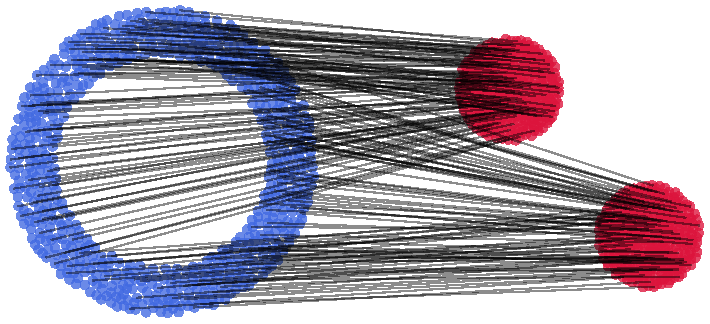
\includegraphics[width=.24\linewidth]{figures/fig-static/static_pairing_p1.pdf}
&
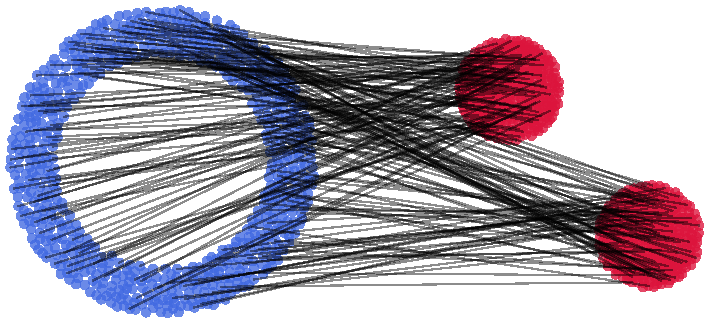
\includegraphics[width=.24\linewidth]{figures/fig-static/static_pairing_pinf.pdf}
&
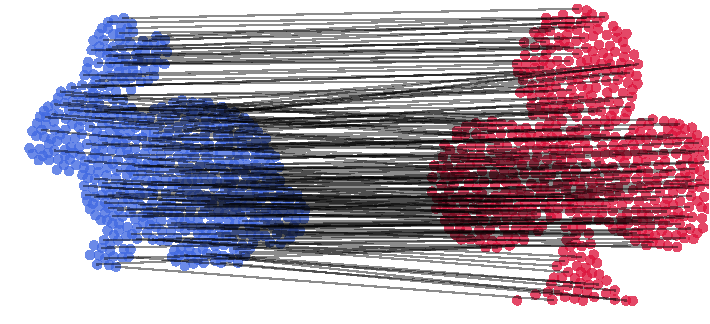
\includegraphics[width=.24\linewidth]{figures/fig-static/bunny-trefle_static_pairing_p1.pdf}
&
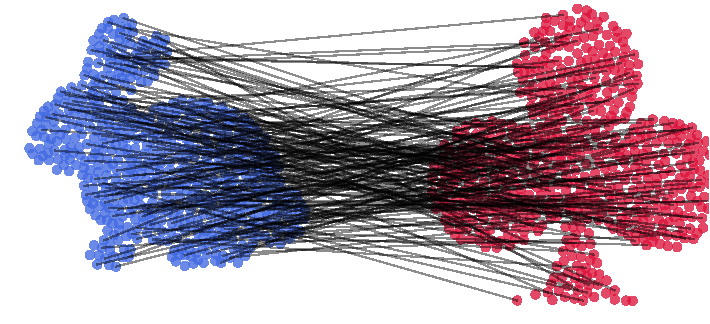
\includegraphics[width=.24\linewidth]{figures/fig-static/bunny-trefle_static_pairing_pinf.pdf}
\\[-.2em]
\scriptsize (a) $p=1$
&
\scriptsize (b) $p=\infty$
&
\scriptsize (c) $p=1$
&
\scriptsize (d) $p=\infty$\\[-2mm]
\end{tabular}
\caption{Static spectral couplings for two source-target pairs. Each pair is shown for $p=1$ and
$p=\infty$, with only a subsample of matched segments displayed.}
\label{fig:static-pair}
\end{figure}




\paragraph{Gaussian setting and Spectral Bures distance.}\label{subsec:gaussians}

Gaussian marginals compress the transport problem to a finite-dimensional optimization over admissible covariance blocks.
%
The proof of the following proposition~\ref{thm:gaussian} and the closed commuting formula for Schatten norms are collected in Appendix~\ref{app:gaussians}.


\begin{proposition}[Gaussian reduction]
\label{thm:gaussian}
Let $\mu=\mathcal N(m_0,\Sigma_0)$ and $\nu=\mathcal N(m_1,\Sigma_1)$. Then $\Wg(\mu,\nu)^2=\inf_K \Big\{ \gamma((m_1-m_0)(m_1-m_0)^\top+\Sigma_0+\Sigma_1-K-K^\top \::\: 
	\left(\begin{smallmatrix}\Sigma_0&K\\K^\top&\Sigma_1\end{smallmatrix}\right)\succeq0 \Big\}$.
\end{proposition}


\section{Dynamic Formulation and Geodesics}
\label{sec:dynamic}
We now turn to the Benamou--Brenier side \citep{BenamouBrenier2000}. This section assumes that $\gamma$ is monotone, so Appendix~\ref{app:matrix-recap} allows us to choose $\cK\subset\mathbb S_+^d$; this positive-semidefinite reduction is the key point in the proof of Theorem~\ref{thm:staticdynamic}, stating the dynamic-static equivalence.

\begin{definition}[Dynamic Spectral Wasserstein]
\label{def:dynamic}
For $\mu_0,\mu_1\in\cP_2(\R^d)$, define $\Wgbb(\mu_0,\mu_1)^2$ as the infimum of $\int_0^1\gamma(\int v_t(x)v_t(x)^\top d\mu_t(x))dt$ over narrowly continuous curves and velocities satisfying $\partial_t\mu_t+\divv(\mu_t v_t)=0$ with endpoints $\mu_0,\mu_1$.
\end{definition}
The equivalent convex momentum formulation is given in Appendix~\ref{app:dynamic-details}.
The following theorem, which is the main result of the paper, states the equivalence between the static and dynamic formulations.  
%
The proof of the theorem and its corollaries are in Appendix~\ref{app:dynamic-details}.


\begin{theorem}[Static-dynamic equivalence]
\label{thm:staticdynamic}
If $\gamma$ is monotone, one has  $\Wgbb(\mu_0,\mu_1)=\Wg(\mu_0,\mu_1)$.
\end{theorem}


\begin{proofsketch}
The detailed argument is given in Appendix~\ref{app:dynamic-details}. For the
dynamic-to-static inequality, let $(\mu_t,v_t)$ solve the continuity equation.
By the superposition principle, it is represented by a probability measure
$\eta$ on absolutely continuous curves, with $\gamma_t{}_\#\eta=\mu_t$ and
$\dot\gamma_t=v_t(\gamma_t)$ for a.e. $t$. The endpoint coupling
$\pi=(\gamma_0,\gamma_1)_\#\eta$ then satisfies
$\gamma_1-\gamma_0=\int_0^1 v_t(\gamma_t)\,dt$ $\eta$-a.e.
%
By monotonicity and Appendix~\ref{app:matrix-recap}, the dual support set
$\cK$ may be chosen in $\mathbb S_+^d$. Hence, for every $Q\in\cK$, Jensen's
inequality gives
$\langle Q,(\gamma_1-\gamma_0)(\gamma_1-\gamma_0)^\top\rangle
\le \int_0^1 \langle Q,v_t(\gamma_t)v_t(\gamma_t)^\top\rangle\,dt$.
Integrating with respect to $\eta$ and taking the supremum over $Q\in\cK$
yields the static cost of $\pi$ bounded by the dynamic action. Taking the
infimum over admissible $(\mu_t,v_t)$ gives one inequality.
%
Conversely, let $\pi$ be an optimal static coupling and set
$\gamma_t=(1-t)x+ty$ for $(x,y)\sim\pi$. Then
$\dot\gamma_t=y-x$, and the induced curve solves the continuity equation. Its
dynamic action equals the static cost of $\pi$, giving the reverse inequality.
\end{proofsketch}


\begin{corollary}[Metric properties]
\label{cor:metric}
$\Wg$ is a distance on $\cP_2(\R^d)$ inducing the same topology as $\Wtwo$.
\end{corollary}

% \begin{proof} Symmetry is obvious. Separation follows from Proposition~\ref{prop:bounds}. The triangle inequality follows from the dynamic formulation by concatenation and time rescaling of admissible curves. \end{proof}

\begin{corollary}[Geodesics]
\label{cor:geodesic}
If $\pi_*$ is any optimal coupling for $\Wg(\mu_0,\mu_1)$, then $\mu_t=((1-t)x+ty)_\#\pi_*$ is a constant-speed geodesic and $\Wg(\mu_s,\mu_t)=|t-s|\,\Wg(\mu_0,\mu_1)$ for every $0\le s\le t\le1$.
\end{corollary}



\begin{figure}[!ht]
\centering
\resizebox{\linewidth}{!}{%
\begin{tabular}{@{}cccccccccc@{}}
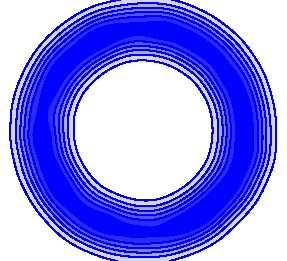
\includegraphics[width=.098\linewidth]{figures/fig-dynamics/static_interp_p1_t0.pdf}
&
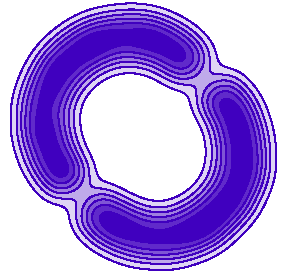
\includegraphics[width=.098\linewidth]{figures/fig-dynamics/static_interp_p1_t1.pdf}
&
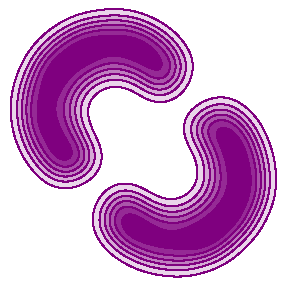
\includegraphics[width=.098\linewidth]{figures/fig-dynamics/static_interp_p1_t2.pdf}
&
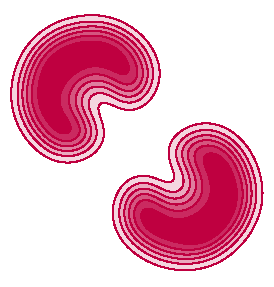
\includegraphics[width=.098\linewidth]{figures/fig-dynamics/static_interp_p1_t3.pdf}
&
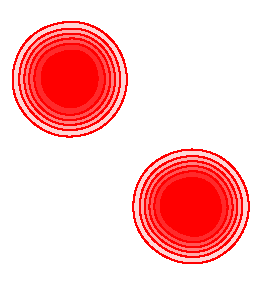
\includegraphics[width=.098\linewidth]{figures/fig-dynamics/static_interp_p1_t4.pdf}
&
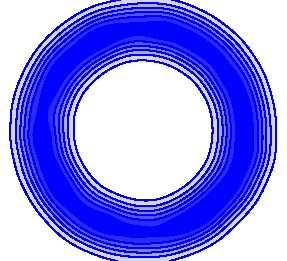
\includegraphics[width=.098\linewidth]{figures/fig-dynamics/static_interp_pinf_t0.pdf}
&
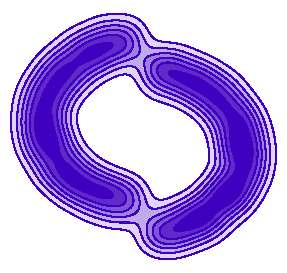
\includegraphics[width=.098\linewidth]{figures/fig-dynamics/static_interp_pinf_t1.pdf}
&
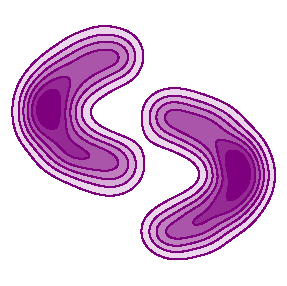
\includegraphics[width=.098\linewidth]{figures/fig-dynamics/static_interp_pinf_t2.pdf}
&
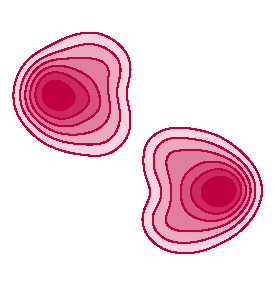
\includegraphics[width=.098\linewidth]{figures/fig-dynamics/static_interp_pinf_t3.pdf}
&
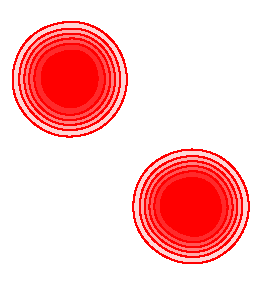
\includegraphics[width=.098\linewidth]{figures/fig-dynamics/static_interp_pinf_t4.pdf}
\\[-.25em]
&
&
\normalsize $p=1$
&
&
&
&
&
\normalsize $p=\infty$
&
&\\[-2mm]
\end{tabular}
}
\caption{Displacement-interpolation density snapshots induced by optimal static couplings, for $p=1$ (first five panels) and for $p=\infty$ (last five panels). We use $n=1500$ particles. As in Figure~\ref{fig:static-pair}, the first and last snapshots correspond to the same source and target distributions ($t=0$ and $t=1$).}
\label{fig:static-interp-dynamic}
\end{figure}

Figure~\ref{fig:static-interp-dynamic} complements Figure~\ref{fig:static-pair}: once an optimal static coupling is fixed, the induced displacement interpolation remains linear in time at the particle level, but the macroscopic density evolution differs markedly between $p=1$ and $p=\infty$. Appendix~\ref{app:extra-static-dynamic} shows additional examples.

\section{Spectral Wasserstein Gradient Flows}
\label{sec:wasserstein-flows}

We now return to the normalized continuity equation introduced in Section~\ref{sec:flows} and explain why, after the static and dynamic theory above, it deserves to be called a Spectral Wasserstein gradient flow.
% Recall the normalized PDE \eqref{eq:measure-spectral-flow}. Before Section~\ref{sec:dynamic}, this was only a normalized transport equation; the Benamou--Brenier identity now identifies $\MN_\mu$ as the infinitesimal norm of $\Wg$.

\paragraph{Metric interpretation of the normalized PDE.}

We now show that \eqref{eq:measure-spectral-flow} is the gradient flow of
$\MF$ for the metric $\Wg$, in the metric-gradient-flow sense of
\citet{AmbrosioGigliSavare2008}.
%
Recall that the metric derivative of an absolutely continuous curve
$t\mapsto\mu_t$ is
$|\mu'|_{\gamma}(t)\coloneqq\lim_{h\to0}\Wg(\mu_{t+h},\mu_t)/|h|$, whenever
the limit exists, and the local slope of $\MF$ is
$|\partial\MF|_{\gamma}(\mu)\coloneqq
\limsup_{\nu\to\mu}(\MF(\mu)-\MF(\nu))_+/\Wg(\mu,\nu)$.
A $\Wg$-gradient flow of $\MF$ is a curve of maximal slope, i.e., a curve
satisfying the energy dissipation identity
$\frac{d}{dt}\MF(\mu_t)
=-\frac12|\mu'|_{\gamma}(t)^2
-\frac12|\partial\MF|_{\gamma}(\mu_t)^2$.

\begin{theorem}[$\Wg$ gradient flow]
\label{prop:formalGF}
If $\gamma$ is monotone and $\MF$ is sufficiently smooth, then
any sufficiently regular solution of \eqref{eq:measure-spectral-flow} is a
 curve of maximal slope for $\MF$ with respect to $\Wg$.
\end{theorem}


\begin{proofsketch}
The detailed proof is in Appendix~\ref{sec:proof-formal-gamma-flow}.
The dynamic formulation identifies the tangent norm associated with $\Wg$ as
the action density $\gamma(\int v v^\top\,d\mu)^{1/2}$. Therefore,
for a smooth curve $(\mu_t,v_t)$ solving the continuity equation, the metric
speed satisfies
$|\dot\mu_t|_{\gamma}^2=\gamma(\int v_t v_t^\top\,d\mu_t )$.
%
Along such a curve, the first variation formula gives
$\frac{d}{dt}\MF(\mu_t)=\int \langle \nabla \frac{\delta \MF}{\delta\mu}(\mu_t), v_t \rangle \,d\mu_t$.
The duality formula for the action norm then yields
$\frac{d}{dt}\MF(\mu_t)\ge
-|\partial \MF|_{\gamma}(\mu_t)\,|\dot\mu_t|_{\gamma}$.
For the vector field prescribed by \eqref{eq:measure-spectral-flow}, equality
holds in this duality bound: the velocity is the Measure-LMO applied to
$\nabla \frac{\delta \MF}{\delta\mu}(\mu_t)$, hence it realizes the steepest
descent direction for the $\Wg$ tangent norm.
%
Consequently,
$-\frac{d}{dt}\MF(\mu_t)
=
|\partial \MF|_{\gamma}(\mu_t)\,|\dot\mu_t|_{\gamma}$,
and the normalization in \eqref{eq:measure-spectral-flow} gives
$|\dot\mu_t|_{\gamma}=|\partial \MF|_{\gamma}(\mu_t)$. Thus, the energy dissipation
identity holds:
$\frac{d}{dt}\MF(\mu_t)=-|\dot\mu_t|_{\gamma}^2=-|\partial \MF|_{\gamma}(\mu_t)^2$.
This is precisely the curve-of-maximal-slope condition for $\MF$ with respect
to $\Wg$.
\end{proofsketch}


\begin{remark}[Insight on Muon's dynamics]\label{rmk:muon-insight}
In the ``Muon setting'', corresponding to the Schatten-$\infty$ gauge
$\gamma(S)=\lambda_{\max}(S)$, the optimality relation
$Q^\star\in\partial\gamma(\Sigma_{\pi^\star})$ stated in Theorem~\ref{thm:minmax} implies that $Q^\star$ is
supported on the top eigenspace of the optimal displacement covariance
$\Sigma_{\pi^\star}$. If this leading eigenspace is one-dimensional (which is the generic situation), say
$\operatorname{span}(u^\star)$, then $Q^\star=u^\star(u^\star)^\top$ and
$\pi^\star$ is optimal for the projected quadratic cost
$\langle y-x,u^\star\rangle^2$.
%
Thus, locally, the Muon mean-field dynamics can be viewed as a Wasserstein
gradient flow in which the relevant ground cost is not the full Euclidean
quadratic cost, but a one-dimensional projected cost selected by the current
largest displacement or velocity covariance direction. In this sense, Muon does
not uniformly penalize all directions of motion. Instead, its geometry
normalizes the dominant direction: the active metric looks only at the direction
where the covariance of the infinitesimal displacement is largest, and the
resulting steepest descent field is obtained by the corresponding projected
optimal-transport geometry. This provides a geometric interpretation of Muon's
orthogonalizing effect: the dynamics continuously identifies the dominant
direction in the mean-field motion and rescales the flow through this
worst-direction cost.
\end{remark}

\paragraph{Mean-field models for two-layer MLPs.}
\label{sec:mlp-meanfield}

We now specialize the abstract gradient-flow PDE to the standard mean-field parameterization of two-layer MLPs.
The mean-field predictor is $H_\mu(z)\coloneqq\int_\Omega \phi(z,x)\,d\mu(x)$, and the training objective is $\MF(\mu)\coloneqq R(H_\mu)$ for some loss $R$.
For a two-layer network with scalar output and activation $\sigma$, one may take parameter $x=(u,v)\in\R^d$ and feature $\phi(z,x)\coloneqq u\,\sigma(v\cdot z)$.
This is the standard mean-field representation of a two-layer multilayer perceptron \citep{MeiMontanariNguyen2018,ChizatBach2018}. 
The notation is a deliberate departure from usual machine-learning conventions: the network input is denoted by $z$, while the trainable variable is denoted by $x$ so that it matches the transport notation used throughout the paper. 
Here $d$ is the sum of the block dimensions of $u$ and $v$. In practical implementations of Muon one often normalizes separate parameter blocks, whereas in our continuum model the whole particle $x$ is treated as a single vector; this is the natural mean-field analogue of a single normalized block. A basic example is the quadratic risk $R(H)=\frac12\int \abs{H(z)-y^\star(z)}^2\,d\rho(z)$, or its empirical version on a dataset. Because $H_\mu$ depends linearly on $\mu$, this makes $\MF(\mu)$ a quadratic interaction functional. These energies are of MMD-type \citep{GrettonBorgwardtRaschSchoelkopfSmola2012}, which is why the MMD experiment below is a natural test case for the Spectral Wasserstein flow.
%
In Figure~\ref{fig:mlp-trajectories}, we train a two-dimensional to
one-dimensional ReLU network, with $\sigma(s)=\max(s,0)$, particles
$x=(u,v_1,v_2)\in\R^3$, and covariates $z\in\R^2$. The target
$y^\star$ is generated by a three-neuron teacher on Gaussian covariates
$z\sim\mathcal N(0,\Id_2)$.
%
To compare the training dynamics for $p=1$ and $p=\infty$ on the same scale,
we rescale time so that the two flows have comparable small-time energy
decay.
%
We display the particle evolution in the reduced two-dimensional plane
$|u|v$. Global convergence corresponds to the concentration of particles
toward the rays associated with the teacher neurons, shown as dashed
half-lines in Figure~\ref{fig:mlp-trajectories}(c)--(d), and can also be
visualized by the convergence of the circular histogram toward three Dirac
masses.
%
Changing $p$ has a strong effect on the early convergence profile, with
$p=\infty$ reaching a significantly lower energy level during the initial
phase.
%
The ReLu case, and more generally, positively two-homogeneous $\phi$ admits a spherical reduction leading to a generalized unbalanced transport geometry; this is described in Appendix~\ref{app:homogeneous}.



\begin{figure}[!th]
\centering
\begin{tabular}{@{}c@{}c@{}c@{}c@{}}
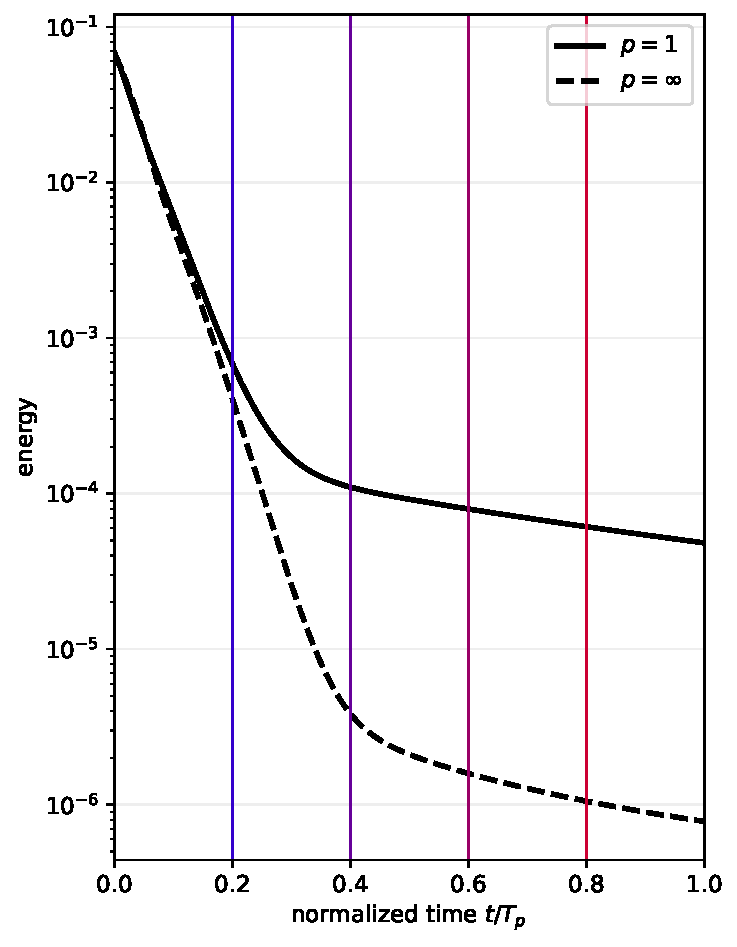
\includegraphics[height=.16\textheight]{figures/fig-mlp/mlp_relu_energy_evolution.pdf}
&
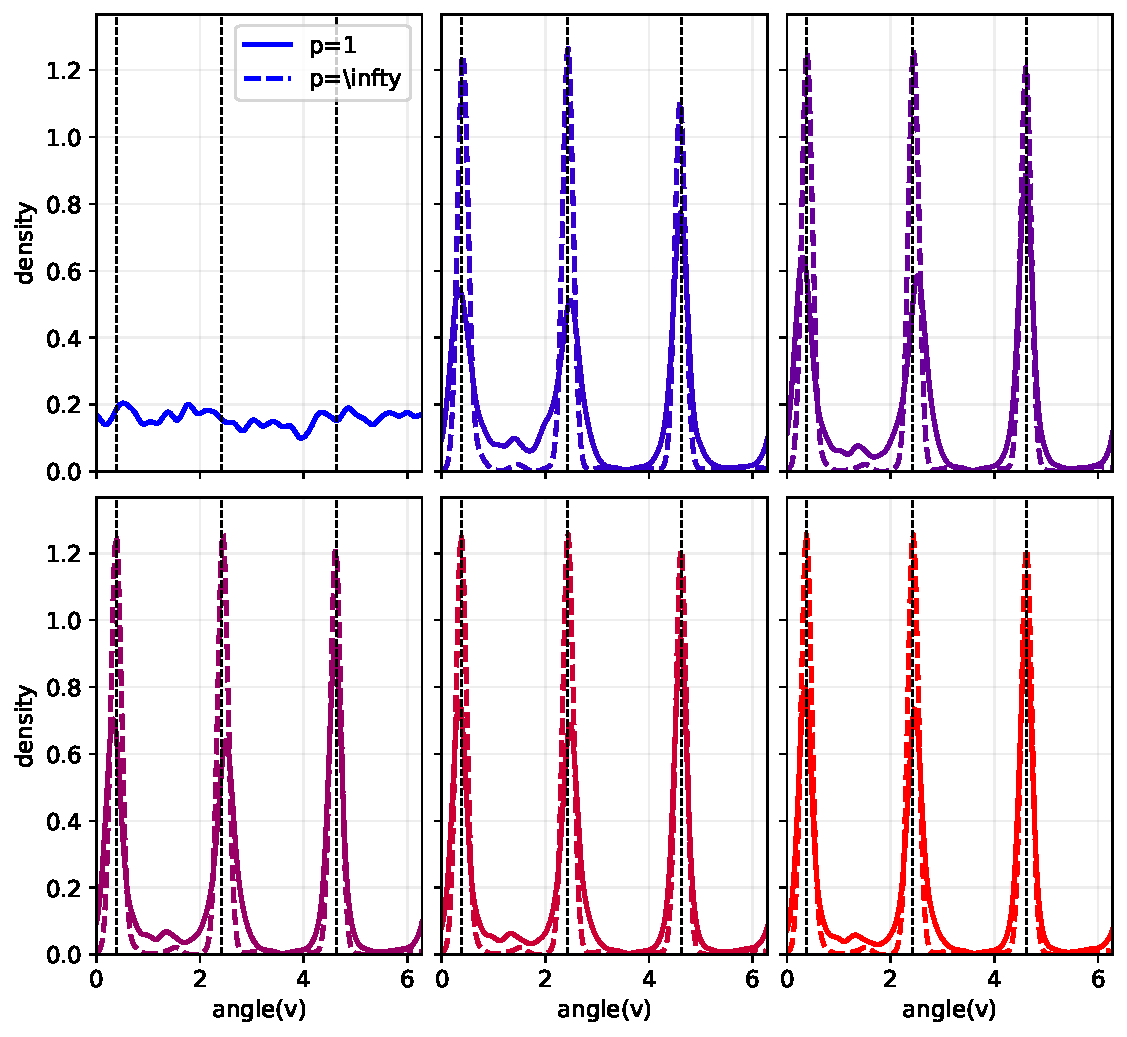
\includegraphics[height=.16\textheight]{figures/fig-mlp/mlp_relu_angular_hist_snapshots_combined.pdf}
&
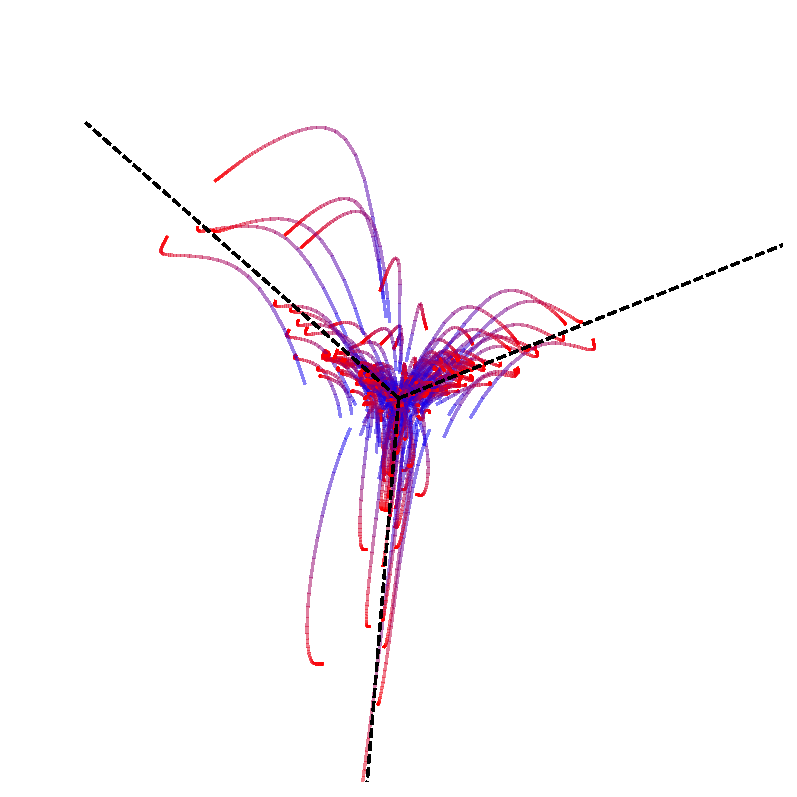
\includegraphics[height=.16\textheight]{figures/fig-mlp/mlp_relu_uvbabs_trajectory_p1.pdf}
&
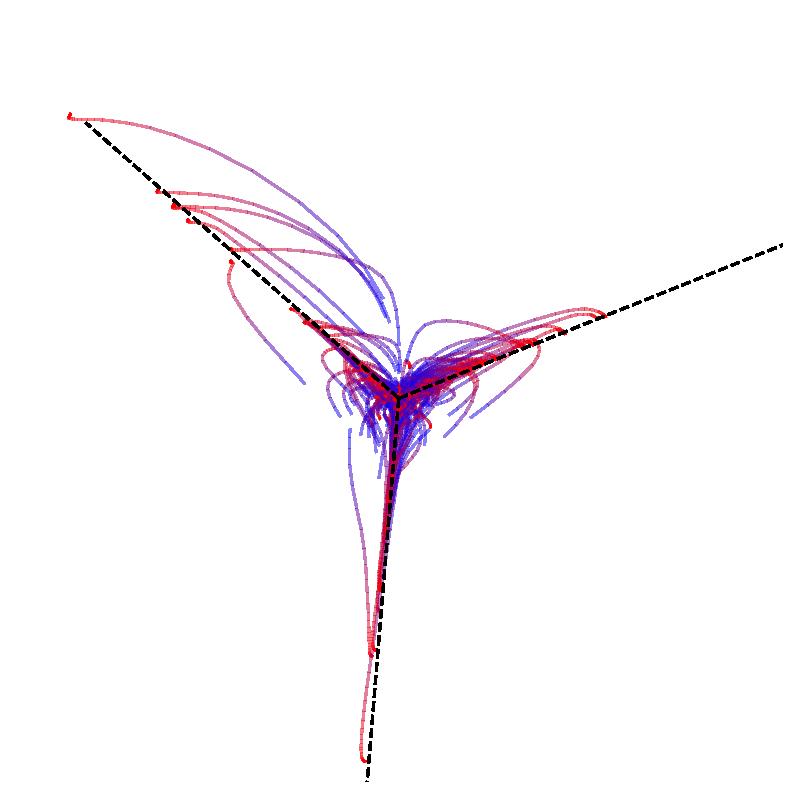
\includegraphics[height=.16\textheight]{figures/fig-mlp/mlp_relu_uvbabs_trajectory_pinf.pdf}
\\
\small (a) Energy decay
&
\small (b) Circular histograms
&
\small (c) Trajectories ($p=1$)
&
\small (d) Trajectories ($p=\infty$)
\end{tabular}
\caption{Two-layer ReLU MLP training under spectral flows. (a) Energy decay in normalized time (solid: $p=1$, dashed: $p=\infty$), with colored vertical bars marking the snapshot times used in (b). (b) Circular histogram snapshots at matched normalized times. (c)--(d) Particle trajectories in the reduced parameter plane $(|u|v_1,|u|v_2)$ for $p=1$ and $p=\infty$.}
\label{fig:mlp-trajectories}
\end{figure}



\paragraph{Mean-field shallow attention.}
Using the same spectral-flow construction, we also consider a shallow mean-field multi-head attention model. This is a useful stress test because attention uses softmax nonlinearities, precisely the regime where Muon-type spectral normalization is empirically attractive. A datum is a sequence $z=(z_1,\ldots,z_m)$ of tokens in $\R^{d_T}$. A head is a particle $x=(Q,K,V,O)$, with $Q,K,V,O\in\R^{d_H\times d_T}$, so $x\in\R^d$ with $d=4d_Hd_T$. Its elementary feature is the softmax attention map $\phi(z,x)_j\coloneqq O^\top\sum_{i=1}^m \frac{\exp(\langle Qz_j,Kz_i\rangle/\sqrt{d_H})}{\sum_{\ell=1}^m\exp(\langle Qz_j,Kz_\ell\rangle/\sqrt{d_H})}Vz_i$, and the mean-field layer is again $H_\mu(z)=\int\phi(z,x)d\mu(x)$. For an empirical measure $\mu_X$, this is a multi-head attention layer averaged over an arbitrary number $n$ of heads, which is the natural mean-field analogue of increasing the number of heads without fixing a finite architecture. 
%%
Figure~\ref{fig:attention-trajectories} reports an experiment with $m=16$ tokens, $d_T=4$, and $d_H=3$: we fit a random five-head teacher by least squares using a student with $n=200$ heads, and compare the trace and operator geometries over five random initializations. The query/key scale controls the sparsity of the teacher attention matrix. We quantify sparsity through the effective number of attended tokens $N_{\mathrm{eff}}\coloneqq(\sum_i w_i^2)^{-1}$ averaged over attention rows: the dense high-temperature regime has $N_{\mathrm{eff}}\approx 16$ out of $m=16$, while the sparse low-temperature regime has $N_{\mathrm{eff}}\approx 2.1$. The $p=1$ and $p=\infty$ horizons are rescaled so that small-time energy decay rates are comparable; even after this normalization, changing $p$ strongly affects the convergence profile and $p=\infty$ reaches a lower energy during the first phase. 

\begin{figure}[!h]
\centering
\begin{tabular}{@{}c@{}c@{}c@{}}
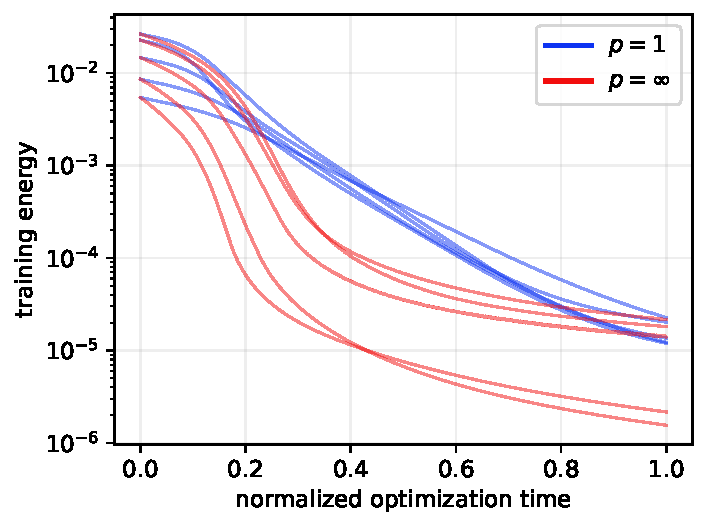
\includegraphics[width=.33\linewidth]{figures/fig-attention/attention_energy_decay_dense.pdf}
&
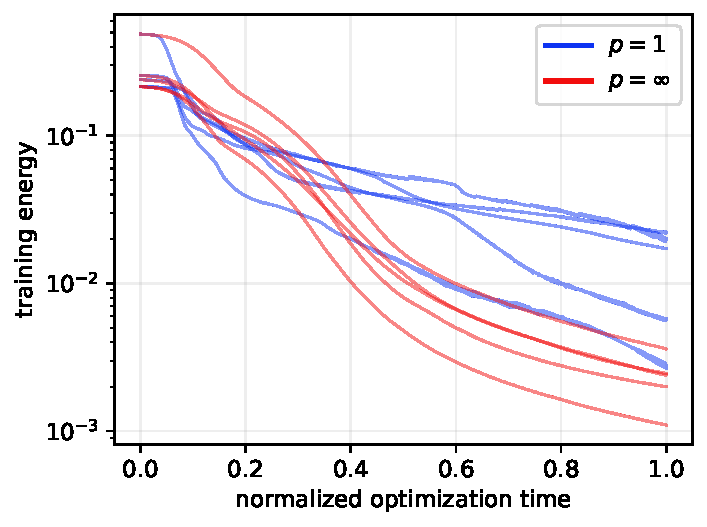
\includegraphics[width=.33\linewidth]{figures/fig-attention/attention_energy_decay_sparse.pdf}
&
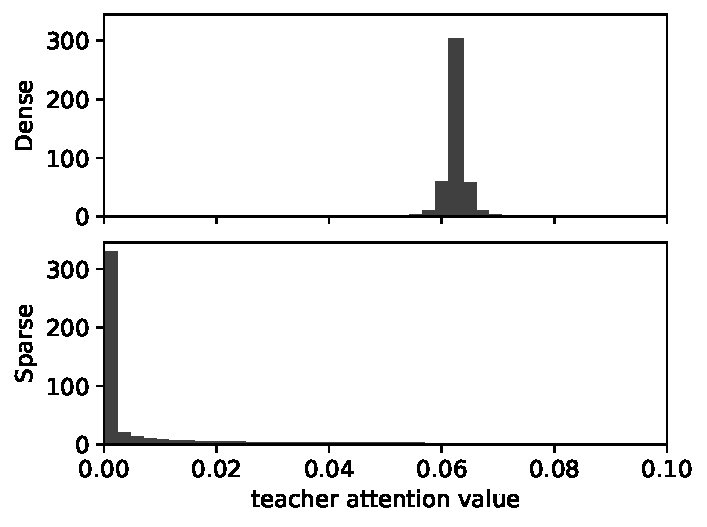
\includegraphics[width=.33\linewidth]{figures/fig-attention/attention_teacher_histograms.pdf}
\\[-2mm]
\small Dense attention
&
\small Sparse attention
&
\small Histogram of teacher attention\\[-2mm]
\end{tabular}
\caption{Shallow-attention training under spectral flows ($p=1$ in blue, $p=\infty$ in red), with five runs per setting. Dense attention corresponds to high temperature and effective support near all tokens ($N_{\mathrm{eff}}\approx16$), while sparse attention corresponds to low temperature and effective support around two tokens ($N_{\mathrm{eff}}\approx2.1$). The right panel stacks the pooled teacher-attention value histograms for the dense and sparse regimes.}
\label{fig:attention-trajectories}
\end{figure}

\paragraph{MMD gradient flows.}
As a simple model for generative fitting and sampling, in the spirit of MMD-based generative models \citep{LiSwerskyZemel2015,BinkowskiSutherlandArbelGretton2018}, we also minimize $\MF(\mu)=\operatorname{MMD}(\mu,\nu)^2$ for the energy-distance kernel $k(x,y)=-\|x-y\|_2$. For empirical measures $\mu=n^{-1}\sum_i\delta_{x_i}$ and $\nu=m^{-1}\sum_j\delta_{y_j}$, with $n=m=200$ particles in $\R^2$, this objective is $\operatorname{MMD}(\mu,\nu)^2=n^{-2}\sum_{i,i'}k(x_i,x_{i'})+m^{-2}\sum_{j,j'}k(y_j,y_{j'})-2(nm)^{-1}\sum_{i,j}k(x_i,y_j)$, with a small smoothing of $\|x-y\|_2$ in the implementation. The same initial cloud evolves with $p=1$ and $p=\infty$.
%
Figure~\ref{fig:mmd-traj} isolates the effect of the spectral tangent norm without the additional architectural structure of a neural network. The trace-norm flow reacts locally to the MMD force field, while the operator-norm flow produces more globally coordinated trajectories; nevertheless, the scalar loss curves remain close.

\begin{figure}[!ht]
\centering
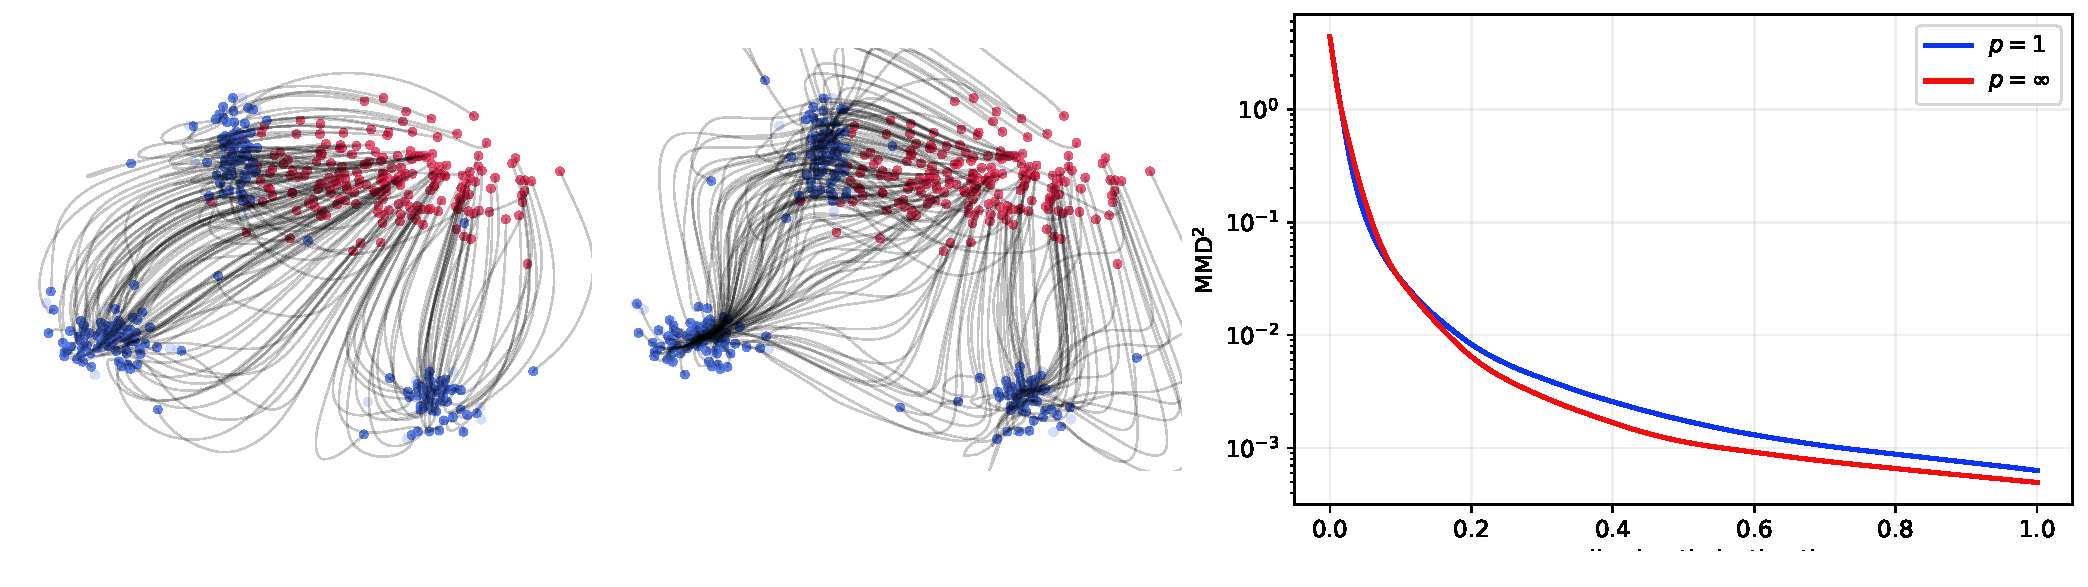
\includegraphics[width=\linewidth]{figures/fig-mmd/mmd_combined_p1_pinf_decay.pdf}\vspace{-3mm}
\caption{MMD flow trajectories and objective decay for $p=1$ and $p=\infty$. The left and middle panels show all particle trajectories, while the right panel shows the decay of $\operatorname{MMD}(\mu_t,\nu)^2$. 
}
\label{fig:mmd-traj}
\end{figure}


\paragraph{Gaussian-preserving linear networks.}\label{sec:gaussian-linear}
To gain a better understanding of spectrally normalized dynamics, a tractable special case is obtained by taking a linear two-layer network, i.e. $\sigma=\Id$, with particles $x=(u,v)$ and predictor $H_\mu(z)=\int (u^\top z)v\,d\mu(u,v)$. For the least-squares risk $R(H)=\frac12\int |H(z)-y^\star(z)|^2d\rho(z)$, the objective depends only on the first two moments of $\mu$. Write $C_\rho\coloneqq\int zz^\top d\rho(z)$ for the data covariance and $B_\rho\coloneqq\int y^\star(z)z^\top d\rho(z)$ for the teacher cross-moment. As explained in Appendix~\ref{app:gaussian-linear},  Gaussian measures are then preserved by the spectral flow, so the infinite-dimensional PDE reduces to an ODE on the mean and covariance. This covariance ODE is still complicated; under simultaneous diagonalization, white-noise balanced initialization, $C_\rho=\Id$, and $B_\rho=\diag(\beta_i)$, it reduces to coupled scalar modes. Writing the modal covariance block as $\Sigma_i(t)=\left(\begin{smallmatrix}s_i(t)&r_i(t)\\ r_i(t)&s_i(t)\end{smallmatrix}\right)$, the coefficient $r_i(t)$ is the learned predictor coefficient in mode $i$, while $s_i(t)$ is the corresponding balanced layer variance.


\begin{proposition}[Commuting Gaussian modal ODE]
\label{prop:modal-main}
Let $q\coloneqq 2p/(2p-1)$, then for each mode $i$,
$
(\dot r_i,\dot s_i)
=
-\mathcal N(r,s)^{2-q}
(r_i-\beta_i)|r_i-\beta_i|^{q-2}
(h^+_i,h^-_i),
$
where $h^\pm_i := (s_i+r_i)^{q/2} \pm (s_i-r_i)^{q/2}$ and 
$\mathcal N(r,s)^q
\coloneqq
\sum_j |r_j-\beta_j|^q
h^+_j$.
\end{proposition}

Note that the coupling factor $\mathcal N(r,s)$ is scalar, so the features
$r_i$ remain decoupled up to a reparametrization of time and can be analyzed
independently.
%
For a rank-one target, the admissible state set is the cone $s>|r|$. The
predictor coefficient $r_t$ moves toward $\beta$, while the terminal value
of $s_t$ records the implicit covariance bias selected by $p$.
Figure~\ref{fig:gaussian-leaves}(a) overlays several such trajectories from two
initial points: all reach the same predictor line $r=\beta$, but at different
covariance levels, revealing a nontrivial $p$-dependent implicit bias.
Panels~(b)--(c) show the conserved leaves that organize these paths for the
endpoint geometries: for $p=1$, the invariant is $s^2-r^2$, whereas for
$p=\infty$, it is $\sqrt{s+r}+\sqrt{s-r}$ (see Appendix~\ref{app:gaussian-linear} for proofs).
%
Panel~(d) shows the impact of $p$ in the rank-two case over the
$(r_1,r_2)$ feature space.

\begin{figure}[!ht]
\centering
\resizebox{\linewidth}{!}{%
\begin{tabular}{@{}c@{}c@{}c@{}c@{}}
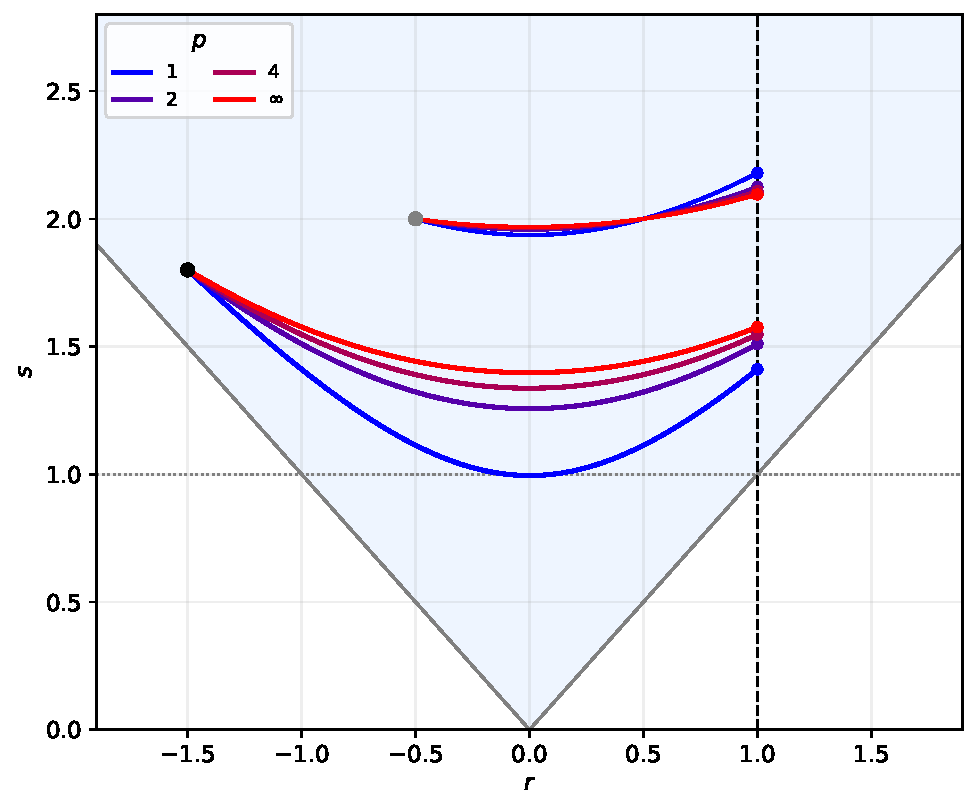
\includegraphics[height=.13\textheight]{figures/fig-gaussians/gaussian_admissible_cone.pdf}
&
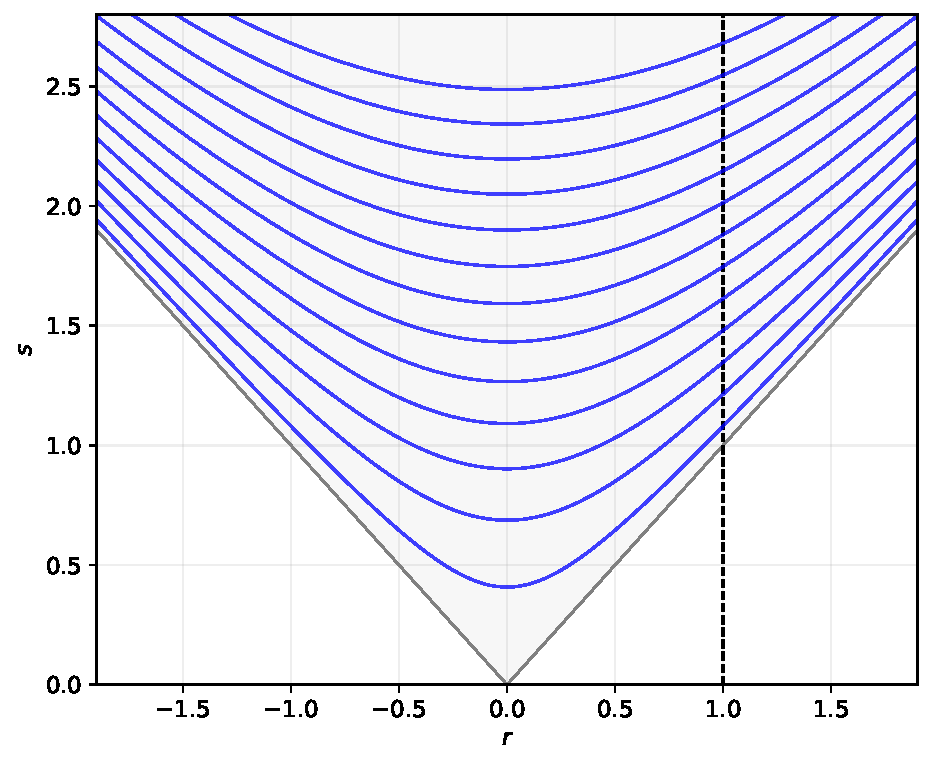
\includegraphics[height=.13\textheight]{figures/fig-gaussians/gaussian_invariant_leaves_p1.pdf}
&
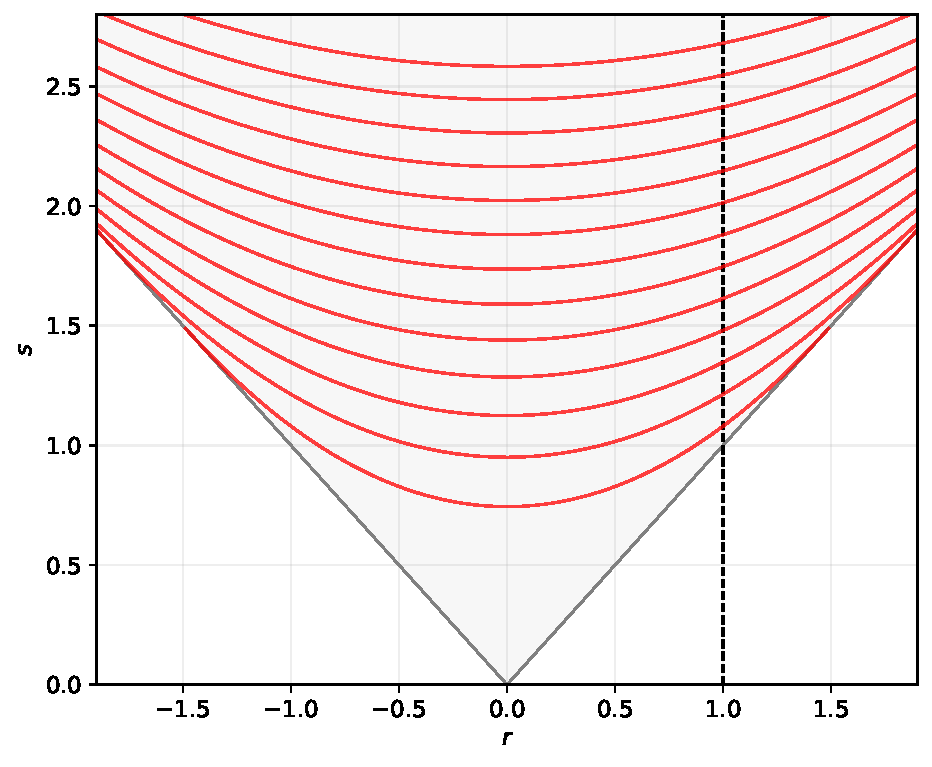
\includegraphics[height=.13\textheight]{figures/fig-gaussians/gaussian_invariant_leaves_pinf.pdf}
&
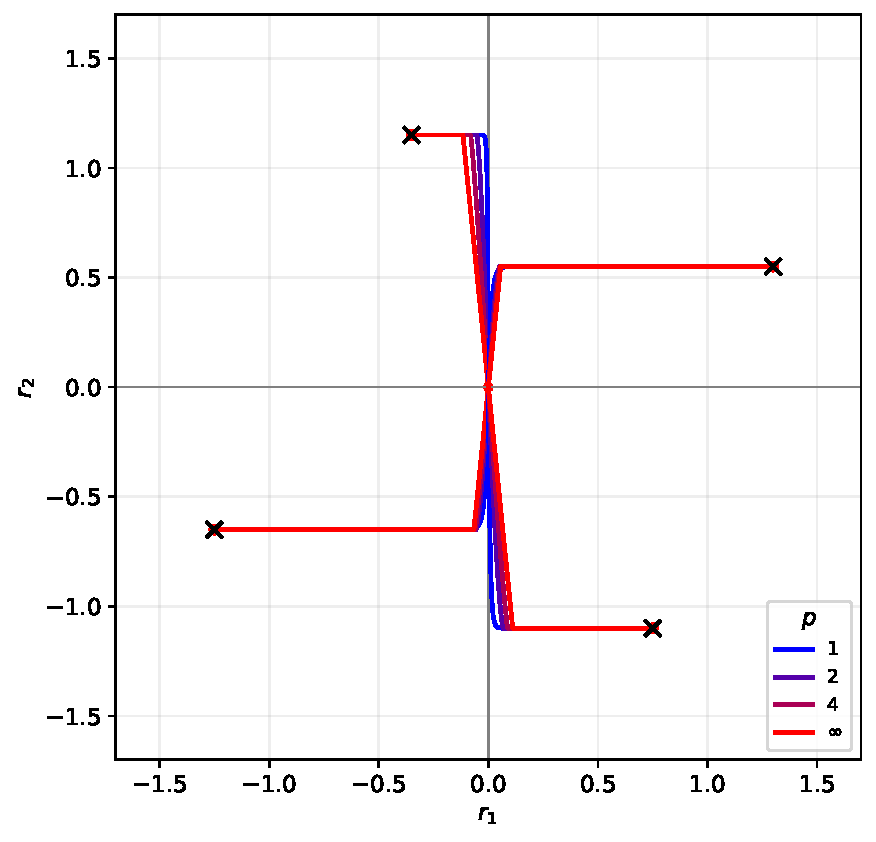
\includegraphics[height=.13\textheight]{figures/fig-gaussians/gaussian_2d_rplane_targets.pdf}
\\[-1mm]
 (a) 1-mode trajectories
&
 (b) Leaves, $p=1$
&
 (c) Leaves, $p=\infty$
&
 (d) 2-mode \\[-2mm]
\end{tabular}
}
\caption{Closed-form Gaussian geometry. Panel (a): one-mode trajectories in $(r,s)$, for $p\in\{1,2,4,\infty\}$. Panels (b)--(c): conserved foliations for the two endpoint geometries. Panel (d): two-mode rank-two dynamics in the $(r_1,r_2)$ plane; all trajectories start from the white-noise state $r_1=r_2=0$, $(s_1,s_2)=(0.1,10)$, and each group targets a different $(\beta_1,\beta_2)$.}
\label{fig:gaussian-leaves}
\end{figure}

\paragraph{Geodesic convexity.}

Geodesic convexity, i.e., the condition
$\mathcal F(\mu_t)\le(1-t)\mathcal F(\mu_0)+t\mathcal F(\mu_1)$ along every
constant-speed $\Wg$-geodesic $(\mu_t)_{t\in[0,1]}$, is a central structural
notion for metric gradient flows \citep{AmbrosioGigliSavare2008}, as it
underlies stability and global convergence results. The following proposition
summarizes several basic convexity examples; Appendix~\ref{app:convexity}
contains the proofs and a refined $\kappa$-geodesic convexity analysis.
%
These results are, however, of limited direct use in the machine-learning
examples considered above, since the quadratic functionals arising in the MLP
and MMD settings are typically not geodesically convex. Note also that
geodesic convexity of the entropy is stated only along a selected geodesic:
uniqueness of geodesics may fail, in particular for $p=\infty$, which makes
the ``muon'' setting is more delicate.

\begin{proposition}[Basic geodesic convexity examples]
\label{prop:basic-geodesic-convexity}
Assume that $\gamma$ is monotone.
%
A linear functional $\mathcal F(\mu)=\int h\,d\mu$, with $h:\R^d\to\R$, is
$\Wg$-geodesically convex if and only if $h$ is convex.
%
A quadratic interaction functional
$\mathcal F(\mu)=\int h(x,y)\,d\mu(x)d\mu(y)$, with
$h:\R^d\times\R^d\to\R$, is $\Wg$-geodesically convex if $h$ is convex.
%
Finally, let $d\nu=Z^{-1}e^{-V}dx$, with $V\in C^2(\R^d)$ convex, and define
the relative entropy by $\mathcal F(\mu)=\int\log(d\mu/d\nu)\,d\mu$ if
$\mu\ll\nu$, and $\mathcal F(\mu)=+\infty$ otherwise. If the representing set
$\cK$ contains at least one positive definite matrix, then for every
$\mu_0,\mu_1\in\cP_2(\R^d)$ there exists a constant-speed $\Wg$-geodesic
$(\mu_t)_{t\in[0,1]}$ joining them along which $\mathcal F$ is convex.
\end{proposition}

\if 0
\begin{proofsketch}
We only sketch the relative entropy case; the detailed proofs are given in
Appendix~\ref{app:convexity}. The only subtlety is that an active matrix in the
robust representation may be singular, preventing a direct reduction to usual
$\Wtwo$ displacement convexity by $x\mapsto Q^{1/2}x$.
%
First suppose that the active matrix $Q_*\in\cK$ is positive definite. Then a
$\Wg$-optimal coupling is optimal for the quadratic cost
$(y-x)^\top Q_*(y-x)$. With $L=Q_*^{1/2}$, the induced interpolation becomes an
ordinary $\Wtwo$-geodesic after pushforward by $L$. Since relative entropy is
invariant under the invertible map $L$, and $V\circ L^{-1}$ is convex, McCann's
displacement convexity theorem gives convexity of $\mathcal F$ along the
corresponding $\Wg$-geodesic.
%
For a general representing set, choose $Q_0\in\cK\cap\Sppd$ and regularize
$\cK$ by $\mathcal K_{\varepsilon}\coloneqq
(1-\varepsilon)\cK+\varepsilon Q_0$. The associated gauges satisfy
$\gamma_{\varepsilon}\to\gamma$ on $\mathbb S_+^d$, while the regularized active
matrices are positive definite. Applying the previous argument to
$\mathsf W_{\gamma_{\varepsilon}}$ and passing to a limit of optimal couplings,
using lower semicontinuity of entropy and convergence of the costs, yields a
constant-speed $\Wg$-geodesic along which $\mathcal F$ is convex.
\end{proofsketch}
\fi 

\section{Conclusion}
\label{sec:conclusion} 

The main message of this paper is that matrix-normalized optimizers for
mean-field neural models are naturally encoded by Spectral Wasserstein
distances. In this view, matrix normalization is not merely a preconditioning
device, but the local steepest-descent geometry generated by a spectral transport
cost. This clarifies the transport side, through coupling-based costs, geodesics,
and Gaussian reductions, and the optimization side, through a continuum
interpretation of normalized matrix updates.
%
The resulting picture is that the choice of spectral gauge shapes which
directions of motion are emphasized or suppressed in the mean-field dynamics,
thereby providing a geometric language for comparing matrix-normalized
optimizers. A major open question is the rigorous study of the Spectral
Wasserstein gradient-flow PDE: global-in-time existence, stability, and the
avoidance of local minima for shallow neural-network and MMD losses.



% \section*{Acknowledgement}
% The author thanks Tony Silveti-Falls, from whom he learned about the intricate details of Muon and with whom he had insightful discussions about Newton--Schulz approximation. This work was supported by the European Research Council (ERC project WOLF) and the French government under the management of Agence Nationale de la Recherche as part of the ``France 2030'' program, reference ANR-23-IACL-0008 (PRAIRIE-PSAI).

\bibliographystyle{plainnat}
\bibliography{references}

\appendix

\section{Matrix Recap and Explicit LMOs}
\label{app:matrix-recap}
This appendix collects the matrix facts used in Section~\ref{sec:flows}. The canonical polar representing set is $\cPol\coloneqq\{Q\in\mathbb S^d:\tr(QS)\le\gamma(S)\text{ for every }S\succeq0\}$; finite-dimensional convex duality gives $\gamma(S)=\max_{Q\in\cPol}\tr(QS)$ for every $S\succeq0$.

We first shows that the use of positive gauges on the cone
$\mathbb S_+^d$ is not essentially more restrictive than working with norms on
the full space of symmetric matrices: under monotonicity, every such gauge
admits a canonical norm extension.

\begin{proposition}[Norm extension of a monotone positive gauge]
\label{prop:gauge-norm-extension}
Let $\gamma:\mathbb S_+^d\to\R_+$ be a monotone positive gauge, i.e.,
$\gamma$ is convex, positively one-homogeneous, $\gamma(S)>0$ for every
nonzero $S\succeq0$, and $0\preceq S\preceq S'$ implies
$\gamma(S)\le\gamma(S')$. Define, for $A\in\mathbb S^d$,
\[
    \|A\|_\gamma
    \coloneqq
    \inf\Bigl\{
        \gamma(P)+\gamma(N):
        P,N\succeq0,\ A=P-N
    \Bigr\}.
\]
Then $\|\cdot\|_\gamma$ is a norm on $\mathbb S^d$, and its restriction to
$\mathbb S_+^d$ coincides with $\gamma$.
\end{proposition}

\begin{proof}
We first note that the admissible set is nonempty for every
$A\in\mathbb S^d$: for instance, the spectral decomposition
$A=A_+-A_-$ gives $A_+,A_-\succeq0$. Hence $\|A\|_\gamma$ is well-defined and
finite.

Positive homogeneity follows directly from the definition. If $a\ge0$, then
\[
    \|aA\|_\gamma
    =
    \inf_{A=P-N}
    \{\gamma(aP)+\gamma(aN)\}
    =
    a\|A\|_\gamma.
\]
If $a<0$, then $aA=(-a)N-(-a)P$ whenever $A=P-N$, so the same argument gives
$\|aA\|_\gamma=|a|\|A\|_\gamma$. In particular, $\|-A\|_\gamma=\|A\|_\gamma$.

We next prove the triangle inequality. Let $A=P_1-N_1$ and $B=P_2-N_2$ with
$P_i,N_i\succeq0$. Then
\[
    A+B=(P_1+P_2)-(N_1+N_2),
\]
and $P_1+P_2,N_1+N_2\succeq0$. By subadditivity of $\gamma$, which follows
from convexity and one-homogeneity,
\[
    \gamma(P_1+P_2)+\gamma(N_1+N_2)
    \le
    \gamma(P_1)+\gamma(P_2)+\gamma(N_1)+\gamma(N_2).
\]
Taking the infimum over all decompositions of $A$ and $B$ yields
$\|A+B\|_\gamma\le\|A\|_\gamma+\|B\|_\gamma$.

It remains to prove nondegeneracy. Since $\gamma$ is strictly positive on the
compact section $\{S\succeq0:\tr(S)=1\}$, there exists $c>0$ such that
$\gamma(S)\ge c\,\tr(S)$ for every $S\succeq0$. Therefore, for every
decomposition $A=P-N$,
\[
    \gamma(P)+\gamma(N)
    \ge
    c\,\tr(P+N).
\]
Moreover, from $A=P-N$ we have $P+N\succeq A$ and $P+N\succeq -A$, which
implies $\tr(P+N)\ge \tr|A|$. Hence
\[
    \gamma(P)+\gamma(N)\ge c\,\tr|A|.
\]
Taking the infimum gives $\|A\|_\gamma\ge c\,\tr|A|$. Thus
$\|A\|_\gamma=0$ implies $A=0$.

Finally, let $S\succeq0$. The decomposition $S=S-0$ gives
$\|S\|_\gamma\le\gamma(S)$. Conversely, if $S=P-N$ with $P,N\succeq0$, then
$P=S+N\succeq S$, and by monotonicity,
$\gamma(P)\ge\gamma(S)$. Hence
\[
    \gamma(P)+\gamma(N)\ge\gamma(P)\ge\gamma(S).
\]
Taking the infimum over all such decompositions gives
$\|S\|_\gamma\ge\gamma(S)$. Therefore $\|S\|_\gamma=\gamma(S)$ for every
$S\succeq0$.
\end{proof}


The next proposition characterizes the monotone norms for which representing sets may be chosen inside the positive-semidefinite cone.
\begin{proposition}[PSD representation and monotonicity]
\label{prop:psdpolar}
The following are equivalent:
\begin{itemize}
\item $\gamma$ is monotone on $\mathbb S_+^d$, namely
$$
0\preceq S\preceq T \Longrightarrow \gamma(S)\le \gamma(T);
$$
\item there exists a convex compact representing set $\cK\subset \mathbb S_+^d$ such that
$$
\gamma(S)=\max_{Q\in \cK}\tr(QS)
\qquad\text{for every }S\succeq 0.
$$
\end{itemize}
Moreover, when these properties hold, the canonical choice
$$
\cK=\cPol\cap \mathbb S_+^d
$$
is admissible.
\end{proposition}

\begin{proof}
If $\cK\subset \mathbb S_+^d$, then for $0\preceq S\preceq T$ one has $\tr(QS)\le \tr(QT)$ for every $Q\in\cK$, hence $\gamma(S)\le \gamma(T)$ by taking suprema.


Conversely, assume $\gamma$ is monotone. Define
$$
\cK^{+}\coloneqq
\{Q\in\mathbb S_+^d:\ \tr(QS)\le \gamma(S)\text{ for every }S\succeq0\}.
$$
It is immediate that $\cK^{+}$ is convex, closed, bounded, and contained in $\cPol\cap\mathbb S_+^d$. We claim that it represents $\gamma$. Fix $S\succeq0$. If $S\succ0$, choose a subgradient $Q\in\partial\gamma(S)$ with respect to the ambient vector space of symmetric matrices. Since $\gamma$ is convex and one-homogeneous, $\tr(QS)=\gamma(S)$ and $\tr(QT)\le\gamma(T)$ for every $T\succeq0$. Moreover $Q\succeq0$: indeed, for every $R\succeq0$ and every sufficiently small $\varepsilon>0$ such that $S-\varepsilon R\succeq0$, the subgradient inequality gives
$$
\gamma(S-\varepsilon R)\ge \gamma(S)-\varepsilon\tr(QR),
$$
while monotonicity gives $\gamma(S-\varepsilon R)\le\gamma(S)$. Hence $\tr(QR)\ge0$ for all $R\succeq0$, i.e. $Q\succeq0$. Thus $Q\in\cK^{+}$ and $\gamma(S)\le\sup_{P\in\cK^{+}}\tr(PS)$. The reverse inequality follows from the definition of $\cK^{+}$. For singular $S\succeq0$, apply the previous argument to $S+\varepsilon I$ and let $\varepsilon\downarrow0$ using continuity of the norm. Therefore $\gamma(S)=\max_{Q\in\cK^{+}}\tr(QS)$ for every $S\succeq0$. Convexity and compactness follow from finite dimensionality.
\end{proof}


\begin{proposition}[Norm property of $\mN$]\label{prop:N-norm}
Assume that $\gamma$ is monotone and admits a positive semidefinite
representing set $\cK\subset\mathbb S_+^d$, so that
$\gamma(S)=\max_{Q\in\cK}\tr(QS)$ for every $S\succeq0$. Define
$\mN(V)\coloneqq\gamma(V^\top V)^{1/2}$. Then $\mN$ is a seminorm. If, in
addition, $\gamma(S)>0$ for every nonzero $S\succeq0$, then $\mN$ is a norm.
\end{proposition}

\begin{proof}
For every matrix $V$, one has
\[
    \mN(V)^2
    =
    \gamma(V^\top V)
    =
    \max_{Q\in\cK}\tr(QV^\top V)
    =
    \max_{Q\in\cK}\tr(VQV^\top).
\]
Since $Q\succeq0$, we may write
$\tr(VQV^\top)=\|VQ^{1/2}\|_F^2$. Hence
\[
    \mN(V)
    =
    \max_{Q\in\cK}\|VQ^{1/2}\|_F.
\]
For each fixed $Q\in\cK$, the map $V\mapsto\|VQ^{1/2}\|_F$ is a seminorm.
Therefore, for any matrices $V,W$ and scalar $a$,
\[
    \mN(aV)
    =
    \max_{Q\in\cK}\|aVQ^{1/2}\|_F
    =
    |a|\mN(V),
\]
and
\[
    \mN(V+W)
    =
    \max_{Q\in\cK}\|(V+W)Q^{1/2}\|_F
    \le
    \max_{Q\in\cK}
    \bigl(\|VQ^{1/2}\|_F+\|WQ^{1/2}\|_F\bigr)
    \le
    \mN(V)+\mN(W).
\]
Thus $\mN$ is a seminorm. If moreover $\gamma(S)>0$ for every nonzero
$S\succeq0$, then $\mN(V)=0$ implies $\gamma(V^\top V)=0$, hence
$V^\top V=0$, and therefore $V=0$. Thus $\mN$ is a norm.
\end{proof}


\begin{remark}[$\mathcal K_\gamma$ for the Schatten $p$-norms]\label{rem-kgamma-shatten}
For $\gamma=\gamma_p$, a convenient supporting set is obtained from the dual
Schatten unit ball. Namely, if $p\in[1,\infty]$ and $q\in[1,\infty]$ is the
conjugate exponent, $1/p+1/q=1$, one may take
\[
    \mathcal K_{\gamma_p}
    =
    \mathcal P_{\gamma_p}\cap\mathbb S_+^d
    \coloneqq
    \Bigl\{
        G\in\mathbb S_+^d:
        \|G\|_{S_q}\leq 1
    \Bigr\}.
\]
One can, however, choose a smaller supporting set in the endpoint cases.
For $p=1$, since $\|A\|_{S_1}=\operatorname{tr}(A)$ on $\mathbb S_+^d$, it is
enough to take $\mathcal K_{\gamma_1}=\{I\}$. For $p=\infty$, one may take the
set of density matrices,
\[
    \mathcal K_{\gamma_\infty}
    =
    \Bigl\{
        G\in\mathbb S_+^d:
        \operatorname{tr}(G)=1
    \Bigr\}.
\]
\end{remark}



The next proposition gives the explicit LMO associated with each Schatten geometry.
\begin{proposition}[Explicit Schatten selectors]
\label{prop:schatten}
Let $\gamma=\gamma_p=\norm{\cdot}_{S_p}$, let $r=2p$, and let $q=\frac{r}{r-1}=\frac{2p}{2p-1}$ be the dual exponent. If
$$
G=U\diag(\sigma_i)W^\top
$$
is the singular value decomposition of a gradient matrix, then
$$
\mJ_p(G)
=
-\norm{G}_{S_q}^{2-q}\,
U\diag(\sigma_i^{q-1})W^\top.
$$
In particular,
\begin{itemize}
\item $p=1$: $\mJ_1(G)=-G$, which recovers ordinary gradient flow;
\item $p=2$: $\mJ_2(G)=-\norm{G}_{S_{4/3}}^{2/3}\,U\diag(\sigma_i^{1/3})W^\top$, which we call the Frobenius-intermediate normalization;
\item $p=\infty$:
\begin{equation}
\label{eq:muon-selector}
\mJ_\infty(G)
=
-\norm{G}_{S_1}\,UW^\top
=
-\tr((G^\top G)^{1/2})\,G\,(G^\top G)^{\dagger/2},
\end{equation}
which is the Muon normalization.
\end{itemize}
\end{proposition}

\begin{proof}
The displayed formula is the negative gradient of $\frac12\norm{G}_{S_q}^2$ when $1<q\le 2$, while the endpoint $q=1$ is interpreted through a subgradient LMO.
\end{proof}


\subsection{Proofs for measure LMOs}
\paragraph{Proof of Theorem~\ref{thm:selector-structure-paper}.}
\begin{proof}
For $Q\in\cK\cap\Sppd$, define
$$
\Phi_Q(v)\coloneqq \int g\cdot v\,d\mu+\frac12\int v^\top Qv\,d\mu.
$$
Since $\gamma(R)=\max_{Q\in\cK}\tr(QR)$ for $R\succeq0$, the Measure-LMO objective is
$$
\inf_v\max_{Q\in\cK}\Phi_Q(v).
$$
For fixed positive definite $Q$, the inner minimization is strictly convex and gives
$$
v_Q(x)=-Q^{-1}g(x),
\qquad
\inf_v\Phi_Q(v)=-\frac12\tr\!\bigl(Q^{-1}\mathcal{S}_\mu(g)\bigr).
$$
The saddle point condition is therefore obtained by choosing $Q_\mu^*$ to maximize this dual value, equivalently to minimize $\tr((Q_\mu^*)^{-1}\mathcal{S}_\mu(g))$. With $v_*(x)=-(Q_\mu^*)^{-1}g(x)$, convex duality gives
$$
\int g\cdot v_*\,d\mu+\frac12\gamma\!\left(\int v_*v_*^\top\,d\mu\right)
=
-\frac12\tr\!\bigl((Q_\mu^*)^{-1}\mathcal{S}_\mu(g)\bigr),
$$
which equals the dual optimum. Thus, $v_*$ minimizes the Measure-LMO objective. The limiting statement follows by lower semicontinuity of the objective in $L^2(\mu)$ along any minimizing sequence whose associated velocities converge.
\end{proof}

\paragraph{Proof of Proposition~\ref{cor:particle}.}
\begin{proof}
For empirical measures, the continuity equation reduces to the characteristic system for the atoms. The identity $\MN_{\mu_X}(v)^2=n^{-1}\mN(V)^2$ and the normalized pairing $n^{-1}\tr(G^\top V)$ reduce the measure-level minimization in Definition~\ref{def:duality} to
$$
\operatorname*{argmin}_V\left\{\tr(G^\top V)+\frac12\mN(V)^2\right\}=\mJ_\gamma(G).
$$
Stacking the particle velocities yields $\dot X_t=\mJ_\gamma(G_t)$. If the matrix objective is $\mF_n(X)=n\MF(\mu_X)$, then $\nabla\mF_n(X)=G_t$, giving the same ODE. If instead $\mF(X)=\MF(\mu_X)$, then $\nabla\mF(X)=n^{-1}G_t$ and one obtains $\dot X_t=n^{-1}\mJ_\gamma(G_t)$ by one-homogeneity of $\mJ_\gamma$. This is exactly the same weak measure equation after rescaling time by $n$.
\end{proof}

\subsection{Comparison between $\Wtwo$ and $\Wg$}
\label{app:static-details}

\paragraph{Proof of Proposition~\ref{prop:bounds}.}
\begin{proof}
Since $\gamma$ is a norm on the finite-dimensional space $\mathbb S^d$, its
restriction to the compact set $\{S\succeq 0:\tr(S)=1\}$ is continuous and
strictly positive. Hence there exist constants
$0<c_\gamma\le C_\gamma<\infty$ such that
$c_\gamma\tr(S)\le \gamma(S)\le C_\gamma\tr(S)$ for every $S\succeq0$.

Let $\pi\in\Pi(\mu,\nu)$ be any coupling, and define its displacement
covariance by
\[
    \Sigma_\pi
    \coloneqq
    \int_{\R^d\times\R^d} (x-y)(x-y)^\top\,d\pi(x,y).
\]
Then $\Sigma_\pi\succeq0$, and therefore
\[
    c_\gamma\tr(\Sigma_\pi)
    \le
    \gamma(\Sigma_\pi)
    \le
    C_\gamma\tr(\Sigma_\pi).
\]
Moreover,
\[
    \tr(\Sigma_\pi)
    =
    \int_{\R^d\times\R^d} \tr\bigl((x-y)(x-y)^\top\bigr)\,d\pi(x,y)
    =
    \int_{\R^d\times\R^d} |x-y|^2\,d\pi(x,y).
\]
Thus, for every coupling $\pi\in\Pi(\mu,\nu)$,
\[
    c_\gamma
    \int |x-y|^2\,d\pi(x,y)
    \le
    \gamma(\Sigma_\pi)
    \le
    C_\gamma
    \int |x-y|^2\,d\pi(x,y).
\]
Taking infima over $\pi\in\Pi(\mu,\nu)$ gives
\[
    c_\gamma \Wtwo(\mu,\nu)^2
    \le
    \Wg(\mu,\nu)^2
    \le
    C_\gamma \Wtwo(\mu,\nu)^2,
\]
where we used the definitions of $\Wtwo$ and $\Wg$. Taking square roots
yields
\[
    \sqrt{c_\gamma}\,\Wtwo(\mu,\nu)
    \le
    \Wg(\mu,\nu)
    \le
    \sqrt{C_\gamma}\,\Wtwo(\mu,\nu).
\]
\end{proof}

\paragraph{Schatten constants and sharpness.}

For Schatten norms, $d^{1/p-1}\,\Wtwo(\mu,\nu)^2\le \mathsf W_{\gamma_p}(\mu,\nu)^2\le \Wtwo(\mu,\nu)^2$, equivalently $c_{\gamma_p}=d^{1/p-1}$ and $C_{\gamma_p}=1$. In particular, $(c_{\gamma_2},C_{\gamma_2})=(d^{-1/2},1)$ and $(c_{\gamma_\infty},C_{\gamma_\infty})=(d^{-1},1)$. These constants follow from $\norm{\lambda}_{\ell_p}\le \norm{\lambda}_{\ell_1}\le d^{1-1/p}\norm{\lambda}_{\ell_p}$.

The lower Schatten bound is sharp. For $\gamma=\gamma_p$, equality in the lower bound is attained by isotropic Gaussian pairs $\mu=\mathcal N(0,\alpha I_d)$ and $\nu=\mathcal N(0,\beta I_d)$, $\alpha,\beta>0$. By the Gaussian computation of Appendix~\ref{app:gaussians}, the displacement covariance is $(\sqrt\alpha-\sqrt\beta)^2I_d$, hence $\mathsf W_{\gamma_p}(\mu,\nu)^2=d^{1/p-1}\Wtwo(\mu,\nu)^2$.


\paragraph{Proof of Theorem~\ref{thm:minmax}.}
\begin{proof}
Let $\pi\in\Pi(\mu,\nu)$ and set
\[
    \Sigma_\pi
    \coloneqq
    \int_{\R^d\times\R^d}
    (y-x)(y-x)^\top\,d\pi(x,y).
\]
Since $\mu,\nu\in\cP_2(\R^d)$, the matrix $\Sigma_\pi$ is well-defined and
belongs to $\mathbb S_+^d$. By the support representation of $\gamma$,
\[
    \gamma(\Sigma_\pi)
    =
    \max_{Q\in\cK}\tr(Q\Sigma_\pi).
\]
Moreover, for every $Q\in\cK$,
\[
    \tr(Q\Sigma_\pi)
    =
    \int_{\R^d\times\R^d}
    (y-x)^\top Q(y-x)\,d\pi(x,y).
\]
Therefore
\[
    \Wg(\mu,\nu)^2
    =
    \inf_{\pi\in\Pi(\mu,\nu)}
    \max_{Q\in\cK}
    \int
    (y-x)^\top Q(y-x)\,d\pi(x,y).
\]

It remains to justify the exchange of $\inf_\pi$ and $\max_Q$. Define
\[
    F(\pi,Q)
    \coloneqq
    \int_{\R^d\times\R^d}
    (y-x)^\top Q(y-x)\,d\pi(x,y).
\]
The coupling set $\Pi(\mu,\nu)$ is convex and weakly compact, since its
marginals are fixed. The set $\cK$ is convex and compact by assumption. For
fixed $\pi$, the map $Q\mapsto F(\pi,Q)$ is affine, hence both concave and
convex, and is continuous on $\cK$. For fixed $Q\succeq0$, the cost
$(x,y)\mapsto (y-x)^\top Q(y-x)$ is nonnegative and lower semicontinuous.
Hence $\pi\mapsto F(\pi,Q)$ is lower semicontinuous for weak convergence of
probability measures, by the Portmanteau theorem. It is also affine in
$\pi$.

Thus the lower-semicontinuous form of Sion's minimax theorem~\cite{sion1958general}  applies and
gives
\[
    \inf_{\pi\in\Pi(\mu,\nu)}
    \max_{Q\in\cK} F(\pi,Q)
    =
    \max_{Q\in\cK}
    \inf_{\pi\in\Pi(\mu,\nu)} F(\pi,Q).
\]
The only point requiring care is that the quadratic cost is not bounded on
$\R^d\times\R^d$. This is precisely why one uses the lower-semicontinuous
version of the minimax theorem rather than the bounded continuous one. 
%
Consequently,
\[
    \Wg(\mu,\nu)^2
    =
    \max_{Q\in\cK}
    \inf_{\pi\in\Pi(\mu,\nu)}
    \int
    (y-x)^\top Q(y-x)\,d\pi(x,y).
\]
Finally, by definition of the quadratic optimal transport cost associated
with $Q$,
\[
    \WQ{Q}(\mu,\nu)^2
    =
    \inf_{\pi\in\Pi(\mu,\nu)}
    \int
    (y-x)^\top Q(y-x)\,d\pi(x,y).
\]
Therefore
\[
    \Wg(\mu,\nu)^2
    =
    \max_{Q\in\cK}\WQ{Q}(\mu,\nu)^2,
\]
which proves the claim.
\end{proof}


\subsection{Metric property from the robust-cost formulation}
\label{subsec:metric-static}

The max--min representation of Theorem~\ref{thm:minmax} gives a direct proof
of the triangle inequality when $\gamma$ is monotone. This avoids using the
Benamou--Brenier formulation for this specific purpose.

\begin{proposition}[Static proof of the metric property]
\label{prop:metric-static}
Assume that $\gamma$ is monotone on $\mathbb S_+^d$. Then $\Wg$ is a distance
on $\cP_2(\R^d)$ and induces the same topology as $\Wtwo$.
\end{proposition}

\begin{proof}
By Proposition~\ref{prop:psdpolar}, monotonicity allows us to choose a
representing set $\cK\subset \mathbb S_+^d$ such that
\[
    \gamma(S)=\max_{Q\in\cK}\tr(QS),
    \qquad S\succeq0.
\]
Hence Theorem~\ref{thm:minmax} gives
\[
    \Wg(\mu,\nu)
    =
    \max_{Q\in\cK}\WQ{Q}(\mu,\nu).
\]
For a fixed $Q\in\cK$, write
\[
    d_Q(x,y)\coloneqq \norm{Q^{1/2}(x-y)}_2 .
\]
Since $Q\succeq0$, $d_Q$ is a seminorm distance on $\R^d$, and therefore
$\WQ{Q}$ is the corresponding quadratic Wasserstein pseudodistance. In
particular, for all $\mu_0,\mu_1,\mu_2\in\cP_2(\R^d)$,
\[
    \WQ{Q}(\mu_0,\mu_2)
    \le
    \WQ{Q}(\mu_0,\mu_1)+\WQ{Q}(\mu_1,\mu_2).
\]
Taking the maximum over $Q\in\cK$ yields
\[
\begin{aligned}
    \Wg(\mu_0,\mu_2)
    &=
    \max_{Q\in\cK}\WQ{Q}(\mu_0,\mu_2) \\
    &\le
    \max_{Q\in\cK}
    \left\{
        \WQ{Q}(\mu_0,\mu_1)+\WQ{Q}(\mu_1,\mu_2)
    \right\} \\
    &\le
    \max_{Q\in\cK}\WQ{Q}(\mu_0,\mu_1)
    +
    \max_{Q\in\cK}\WQ{Q}(\mu_1,\mu_2) \\
    &=
    \Wg(\mu_0,\mu_1)+\Wg(\mu_1,\mu_2).
\end{aligned}
\]
Symmetry is immediate from the definition. Moreover $\Wg(\mu,\mu)=0$, and
separation follows from Proposition~\ref{prop:bounds}: if $\Wg(\mu,\nu)=0$,
then $\Wtwo(\mu,\nu)=0$, hence $\mu=\nu$. The same comparison bounds also show
that $\Wg$ and $\Wtwo$ induce the same topology on $\cP_2(\R^d)$.
\end{proof}

\begin{remark}[Relation with subspace robust Wasserstein distances]
\label{rem:paty-cuturi-metric-proof}
The proof is the same robust-cost argument used by
\citet{PatyCuturi2019} for Ky Fan gauges. The only point needed in their
argument is that the maximizing cost matrices are positive semidefinite. By
Proposition~\ref{prop:psdpolar}, this positivity holds for any monotone gauge
$\gamma$, not only for Ky Fan gauges. Thus the Paty--Cuturi triangle-inequality
proof extends verbatim to the present monotone-gauge setting.
\end{remark}


\subsection{Large-mean asymptotics for Schatten geometries}
\label{subsec:large-mean-schatten}

We now describe the behavior of $\Wg$ when the displacement between the means
is much larger than the centered fluctuations of the measures. This regime is
useful to interpret the optimizer in the max-min formula: for Schatten
geometries with $p>1$, the optimal certificate becomes increasingly aligned
with the direction of the mean displacement, and the residual transport
problem is effectively measured only along this direction.

\begin{proposition}[Large-mean asymptotics for Schatten geometries]
\label{prop:large-mean-schatten}
Let $\gamma=\gamma_p$ be the Schatten-$p$ norm, with $p\in[1,\infty]$, and let
$\mu,\nu\in\cP_2(\R^d)$. Set
$m_\mu\coloneqq\int x\,d\mu(x)$, $m_\nu\coloneqq\int x\,d\nu(x)$, and
$\Delta\coloneqq m_\nu-m_\mu$. Assume $\Delta\neq0$, and write
$\Delta=Ru$, where $R=\abs{\Delta}$ and $u=\Delta/\abs{\Delta}$. Let
$\bar\mu\coloneqq(\Id-m_\mu)_\#\mu$ and
$\bar\nu\coloneqq(\Id-m_\nu)_\#\nu$. Then, as $R\to\infty$ with
$\bar\mu,\bar\nu$ fixed, the following asymptotics hold.
%
For $p=1$, 
\[
    \Wg(\mu,\nu)^2
    =
    R^2+\Wtwo(\bar\mu,\bar\nu)^2 .
\]
For $1<p\le\infty$,
\[
    \Wg(\mu,\nu)^2
    =
    R^2+\WQ{uu^\top}(\bar\mu,\bar\nu)^2+o(1).
\]
\end{proposition}

\begin{proof}
We first separate the mean displacement from the centered transport. Fix
$Q\succeq0$. If $\pi\in\Pi(\mu,\nu)$ and if $\bar\pi$ denotes the corresponding
coupling of $\bar\mu$ and $\bar\nu$, then writing
$x=m_\mu+\bar x$ and $y=m_\nu+\bar y$ gives
\[
    y-x=\Delta+(\bar y-\bar x).
\]
Therefore
\[
\begin{aligned}
    \int (y-x)^\top Q(y-x)\,d\pi(x,y)
    &=
    \Delta^\top Q\Delta
    +
    2\Delta^\top Q
    \int(\bar y-\bar x)\,d\bar\pi(\bar x,\bar y) \\
    &\qquad
    +
    \int(\bar y-\bar x)^\top Q(\bar y-\bar x)\,
    d\bar\pi(\bar x,\bar y).
\end{aligned}
\]
The middle term vanishes because $\bar\mu$ and $\bar\nu$ have zero mean. Taking
the infimum over couplings yields the exact decomposition
\[
    \WQ{Q}(\mu,\nu)^2
    =
    \Delta^\top Q\Delta+\WQ{Q}(\bar\mu,\bar\nu)^2.
\]
By Theorem~\ref{thm:minmax},
\[
    \Wg(\mu,\nu)^2
    =
    \max_{Q\in\mathcal K_{\gamma_p}}
    \left\{
        \Delta^\top Q\Delta+\WQ{Q}(\bar\mu,\bar\nu)^2
    \right\}.
\]

For $p=1$, we use the reduced representing set
$\mathcal K_{\gamma_1}=\{\Id\}$. Then
\[
    \Wg(\mu,\nu)^2
    =
    \Delta^\top\Delta+\WQ{\Id}(\bar\mu,\bar\nu)^2
    =
    R^2+\Wtwo(\bar\mu,\bar\nu)^2,
\]
as claimed.

Assume now that $1<p\le\infty$, and let $q$ be the conjugate exponent, with
$q=1$ when $p=\infty$. We use the positive dual Schatten representing set
\[
    \mathcal K_{\gamma_p}
    =
    \{Q\succeq0:\norm{Q}_{S_q}\le1\}.
\]
Since $\Delta=Ru$, the max-min formula becomes
\[
    \Wg(\mu,\nu)^2
    =
    \max_{Q\in\mathcal K_{\gamma_p}}
    \left\{
        R^2 u^\top Q u+\WQ{Q}(\bar\mu,\bar\nu)^2
    \right\}.
\]
By Schatten duality, applied to the rank-one matrix $uu^\top$,
\[
    \max_{Q\in\mathcal K_{\gamma_p}} u^\top Q u
    =
    \max_{\substack{Q\succeq0\\ \norm{Q}_{S_q}\le1}}
    \tr(Q\,uu^\top)
    =
    \norm{uu^\top}_{S_p}
    =
    1.
\]
For $1<p<\infty$, the equality case in Hölder's inequality is unique and gives
$Q=uu^\top$. For $p=\infty$, the constraint is $\tr(Q)\le1$, and
$u^\top Q u\le\tr(Q)\le1$; equality again forces $Q=uu^\top$. Thus the exposed
face of $\mathcal K_{\gamma_p}$ in the direction $uu^\top$ is the singleton
$\{uu^\top\}$ for every $1<p\le\infty$.

Let $Q_R$ be an optimal certificate for the previous maximization problem.
Since $\mathcal K_{\gamma_p}$ is compact, any sequence $R_n\to\infty$ admits a
subsequence such that $Q_{R_n}\to Q_\infty\in\mathcal K_{\gamma_p}$. Dividing
the optimality relation by $R_n^2$ and passing to the limit shows that
$Q_\infty$ maximizes $Q\mapsto u^\top Q u$ over $\mathcal K_{\gamma_p}$. By
the uniqueness of the exposed maximizer, $Q_\infty=uu^\top$. Hence every
maximizing certificate satisfies
\[
    Q_R\longrightarrow uu^\top
    \qquad\text{as }R\to\infty.
\]
Since $Q\mapsto\WQ{Q}(\bar\mu,\bar\nu)^2$ is continuous on
$\mathcal K_{\gamma_p}$, we obtain
\[
    \WQ{Q_R}(\bar\mu,\bar\nu)^2
    \longrightarrow
    \WQ{uu^\top}(\bar\mu,\bar\nu)^2.
\]
Substituting this into the max-min formula gives
\[
    \Wg(\mu,\nu)^2
    =
    R^2+\WQ{uu^\top}(\bar\mu,\bar\nu)^2+o(1).
\]
Taking square roots yields
\[
    \Wg(\mu,\nu)
    =
    R+\frac{1}{2R}\WQ{uu^\top}(\bar\mu,\bar\nu)^2+o(R^{-1}),
\]
which completes the proof.
\end{proof}

The proposition shows that all Schatten geometries have the same leading
large-mean behavior, namely $\Wg(\mu,\nu)\sim\abs{\Delta}$. The difference
appears at the next order and in the optimizer selected by the max-min
formula. For the reduced trace geometry $p=1$, the certificate is fixed and
isotropic, $Q=\Id$, so the centered correction is the usual Wasserstein cost
$\Wtwo(\bar\mu,\bar\nu)^2$. By contrast, for every $p>1$, the optimal
certificate aligns with the normalized mean displacement
$u=\Delta/\abs{\Delta}$, and the centered correction becomes
$\WQ{uu^\top}(\bar\mu,\bar\nu)^2$. Thus, in the large-mean regime, the
coupling selected by the Schatten geometry is increasingly influenced by the
one-dimensional projection along $u$: transverse fluctuations only affect the
cost at lower order through the way they interact with the projected
quadratic transport problem.



\section{Connection with Muon, Orthogonalization, and Momentum}
\label{sec:muon-extensions}
This appendix complements Section~\ref{sec:flows} by linking the matrix ODE for $p=\infty$ to practical Muon variants used at scale, and by showing how Newton--Schulz orthogonalization and momentum fit in the same normalized-flow language.

\paragraph{Taking into account Newton--Schulz orthogonalization.}
Setting $p=\infty$ in Proposition~\ref{prop:schatten} yields the LMO \eqref{eq:muon-selector}, so the spectral matrix flow
$$
\dot X_t=\mJ_\infty(\nabla \mF(X_t))
$$
is exactly the vanishing-step-size, vanishing-momentum, full-batch limit of idealized Muon in the normalization convention used throughout this paper.

An important practical feature of Muon is that one does not compute the exact polar factor $UW^\top$ by an SVD at every step. To make the method scalable and GPU-friendly, practical implementations replace $UW^\top = G(G^\top G)^{\dagger/2}$ by a few Newton--Schulz iterations \citep{KellerJordan2024,LiuSuYaoEtAl2025}. After rescaling $G$ by a scalar $\alpha(G)>0$ chosen so that the spectrum of $\alpha(G)^{-2}G^\top G$ lies in $[0,1]$, the classical Newton--Schulz iteration reads
$$
Z_{k+1}
=
\frac12 Z_k(3I-Z_k^\top Z_k),
\qquad
Z_0=\alpha(G)^{-1}G.
$$
For the discussion below, let us freeze the scale and regard $\alpha>0$ as fixed a priori. Then after one iteration one obtains
$$
\mJ_{\alpha,1}(G)
\coloneqq
-Z_1
=
-\frac{1}{2\alpha}
\,G\left(3I-\alpha^{-2}G^\top G\right),
$$
and after $k$ iterations one obtains more generally a polynomial LMO of the form
$$
\mJ_{\alpha,k}(G)
=
-G\,p_{\alpha,k}\!\left(G^\top G\right),
$$
where $p_{\alpha,k}$ is a matrix polynomial approximating $s\mapsto s^{-1/2}$ on the spectral interval of interest. In this fixed-$\alpha$ setting, the polynomial orthogonalization part does admit a scalar generating function: if
$$
p_{\alpha,k}(s)=\sum_{\ell=0}^m a_\ell s^\ell,
$$
then
$$
\gamma_{\alpha,k}(S)\coloneqq \sum_{\ell=0}^m \frac{a_\ell}{\ell+1}\tr(S^{\ell+1})
$$
satisfies
$$
\nabla \gamma_{\alpha,k}(S)=p_{\alpha,k}(S)
\qquad\text{and}\qquad
\mJ_{\alpha,k}(G)
=
-\nabla_G\!\left(\frac12 \gamma_{\alpha,k}(G^\top G)\right).
$$
For one Newton--Schulz step this gives the explicit formula
$$
\gamma_{\alpha,1}(S)
=
\frac{3}{2\alpha}\tr(S)-\frac{1}{4\alpha^3}\tr(S^2).
$$
This function is not a norm, and it is not globally monotone on $\mathbb S_+^d$, because
$$
\nabla \gamma_{\alpha,1}(S)=\frac{3}{2\alpha}I-\frac{1}{2\alpha^3}S
$$
ceases to be positive semidefinite once $S$ has eigenvalues larger than $3\alpha^2$. It is nevertheless monotone on the truncated spectral region
$$
0\preceq S\preceq 3\alpha^2 I,
$$
and in particular on the standard Newton--Schulz regime $0\preceq S\preceq \alpha^2 I$.

Therefore, if one replaces the exact Muon LMO $\mJ_\infty$ by the fixed-$\alpha$ Newton--Schulz LMO $\mJ_{\alpha,k}$, the resulting approximate Muon dynamics is again generated by a spectral functional, now $\gamma_{\alpha,k}$. The main caveat is that in practical implementations the scaling parameter $\alpha$ is not frozen but chosen adaptively from the current matrix in order to track the evolving spectrum during training. Extending the present geometric interpretation to that state-dependent choice of $\alpha$ remains an open question.

\paragraph{Taking into account momentum.}
A natural momentum extension, in the spirit of Muon with exponential moving average, is obtained by introducing an auxiliary matrix variable $A_t$ and considering
\begin{equation}
\label{eq:matrix-momentum}
\tau \dot A_t + A_t = \nabla \mF(X_t),
\qquad
\dot X_t = \mJ_\gamma(A_t),
\end{equation}
where $\tau\ge 0$ is the memory time scale. The variable $A_t$ plays the role of a continuous-time exponentially averaged gradient. When $\tau=0$, one recovers exactly the first-order spectral flow studied above.

For smooth Schatten geometries ($1<p<\infty$), this system is equivalent to a second-order inertial equation
$$
\tau \frac{d}{dt}\bigl(\mI_p(\dot X_t)\bigr) + \mI_p(\dot X_t) + \nabla \mF(X_t)=0,
$$
where
$$
\mI_p(V)
\coloneqq
\norm{V}_{S_r}^{2-r}\,U\diag(\sigma_i^{r-1})W^\top,
\qquad r=2p,
$$
for $V=U\diag(\sigma_i)W^\top$. In particular, for $p=1$ one has $\mI_1(V)=V$ and one recovers the heavy-ball equation
$$
\tau \ddot X_t + \dot X_t + \nabla \mF(X_t)=0.
$$
At the endpoint $p=\infty$, \eqref{eq:matrix-momentum} reads
$$
\tau \dot A_t + A_t = \nabla \mF(X_t),
\qquad
\dot X_t = -\norm{A_t}_{S_1}\,U_tW_t^\top,
$$
which is the exact-polar continuous-time Muon dynamics with momentum.

The corresponding mean-field description naturally lives on phase space. Let
$$
\eta_t\in\cP_2(\R^d\times\R^d)
$$
be the law of pairs $(x,a)$, where $x$ is the particle position and $a$ is the exponentially averaged force. Its spatial marginal is
$$
\mu_t=(\pi_x)_\#\eta_t.
$$
For a functional $\MF$ on measures, write its Wasserstein force as
$$
g_\mu(x)=\nabla_x\frac{\delta\MF}{\delta\mu}(x).
$$
Given a phase-space law $\eta$, define the momentum covariance
$$
S(\eta)\coloneqq
\int_{\R^d\times\R^d}aa^\top\,d\eta(x,a).
$$
In the monotone regime, and assuming for simplicity that an invertible inverse-trace minimizer can be selected, choose
$$
Q_\eta^*\in\operatorname*{argmin}_{Q\in\cK\cap\Sppd}\tr\!\bigl(Q^{-1}S(\eta)\bigr).
$$
The phase-space characteristics are then
\begin{equation}
\label{eq:phase-momentum-characteristics}
\dot x_t=-(Q_{\eta_t}^*)^{-1}a_t,
\qquad
\tau\dot a_t=g_{\mu_t}(x_t)-a_t .
\end{equation}
Consequently, the law $\eta_t$ solves the Liouville-type equation
\begin{equation}
\label{eq:phase-momentum-liouville}
\partial_t\eta_t
+\operatorname{div}_x(\eta_t u_t)
+\frac1\tau\operatorname{div}_a\!\bigl(\eta_t(g_{\mu_t}(x)-a)\bigr)=0,
\end{equation}
where
$$
u_t(x,a)=-(Q_{\eta_t}^*)^{-1}a,
\qquad
\mu_t=(\pi_x)_\#\eta_t.
$$
When $\tau=0$, the averaged force instantaneously relaxes to $a=g_{\mu_t}(x)$, and the spatial marginal formally recovers the first-order normalized PDE \eqref{eq:measure-spectral-flow}. For $\tau>0$, the dynamics is no longer a metric gradient flow for $\Wg$ on the position marginal alone; it is a damped kinetic system in which the spectral geometry enters through the constitutive relation between the phase-space force covariance and the spatial velocity.

\section{Monge Maps and Conditional Brenier Theorem}
\label{app:monge}
This appendix collects the map-based statements associated with the static formulation of Section~\ref{sec:static}.

The next definition records the Monge restriction, which is useful for comparison but is not the correct notion in general.
\begin{definition}[Monge restriction]
\label{def:monge}
Define
$$
\WgM(\mu,\nu)^2
\coloneqq 
\inf_{T_\#\mu=\nu}
\gamma\!\left(
\int_{\R^d}(T(x)-x)(T(x)-x)^\top\,d\mu(x)
\right),
$$
with value $+\infty$ if no transport map exists.
\end{definition}

The next proposition simply records that the map-based problem is a restriction of the coupling-based one.
\begin{proposition}[Monge is a restriction]
\label{prop:monge}
For every $\mu,\nu\in\cP_2(\R^d)$,
$$
\Wg(\mu,\nu)\le \WgM(\mu,\nu).
$$
\end{proposition}

\begin{proof}
Every transport map $T$ induces the coupling $(\Id,T)_\#\mu$, and the static cost evaluated on this coupling is exactly the Monge cost associated with $T$.
\end{proof}

The following remark shows on a two-Dirac example that the relaxation can be genuinely strict.
\begin{remark}[Strictness of the Monge restriction]
Consider
$$
\mu=\frac12(\delta_{(-1,0)}+\delta_{(1,0)}),
\qquad
\nu=\frac12(\delta_{(0,-1)}+\delta_{(0,1)}).
$$
Any transport map from $\mu$ to $\nu$ is a bijection between the two atoms. The two possible displacement covariance matrices are
$$
\begin{pmatrix}
1 & 1\\
1 & 1
\end{pmatrix}
\qquad\text{or}\qquad
\begin{pmatrix}
1 & -1\\
-1 & 1
\end{pmatrix},
$$
so for the operator norm and Frobenius norm one gets
$$
\WgM(\mu,\nu)^2=2.
$$
By contrast, the split coupling assigning mass $1/4$ to each source-target pair has displacement covariance equal to the identity matrix, hence
$$
\Wg(\mu,\nu)^2=
1
\quad\text{for }\gamma=\norm{\cdot}_{S_\infty},
\qquad
\Wg(\mu,\nu)^2=
\sqrt{2}
\quad\text{for }\gamma=\norm{\cdot}_{S_2}.
$$
Therefore the inequality in Proposition~\ref{prop:monge} is strict already for two-point measures.
\end{remark}

The next remark explains that, for a completely arbitrary norm on $\mathbb S_+^d$, the static cost need not yet be a bona fide metric.
\begin{remark}[Triangle inequality may fail for non-monotone norms]
\label{rem:notmetric}
For Dirac masses, the unique coupling gives
$$
\Wg(\delta_x,\delta_y)^2
=
\gamma\!\left((y-x)(y-x)^\top\right).
$$
Hence if $\Wg$ were always a distance, then the pointwise cost
$$
d_\gamma(x,y)
\coloneqq 
\sqrt{\gamma\!\left((y-x)(y-x)^\top\right)}
$$
would in particular have to define a metric on $\R^d$.

This fails for general norms on $\mathbb S_+^d$. Fix $d\ge 2$ and a parameter $M>2$, and define
$$
\gamma_{\mathrm{ns}}(S)
\coloneqq 
\tr(S)+M\sum_{1\le i<j\le d}\abs{S_{ij}},
\qquad S\succeq 0.
$$
This is a norm on $\mathbb S_+^d$, but it is not spectral since it depends on the matrix entries and not only on the eigenvalues. For the displacement
$$
\Delta=y-x=(\Delta_1,\dots,\Delta_d)
$$
one has
$$
d_{\gamma_{\mathrm{ns}}}(x,y)^2
=
\norm{\Delta}_2^2
+
M\sum_{1\le i<j\le d}\abs{\Delta_i\Delta_j}.
$$
Taking
$$
x_0=0,
\qquad
x_1=e_1,
\qquad
x_2=e_1+e_2
$$
gives
$$
d_{\gamma_{\mathrm{ns}}}(x_0,x_1)=1,
\qquad
d_{\gamma_{\mathrm{ns}}}(x_1,x_2)=1,
\qquad
d_{\gamma_{\mathrm{ns}}}(x_0,x_2)=\sqrt{2+M}>2,
$$
so the triangle inequality fails.

By contrast, if $\gamma$ is monotone on $\mathbb S_+^d$, then Proposition~\ref{prop:psdpolar} allows us to choose $\cK\subset \mathbb S_+^d$, and therefore
$$
d_\gamma(x,y)
=
\sup_{Q\in\cK}\norm{Q^{1/2}(x-y)}_2,
$$
which is a supremum of seminorms and therefore a genuine distance on $\R^d$. For general measures, however, this pointwise argument does not control the cross terms created by gluing couplings. The full metric property of $\Wg$ in the monotone case is therefore proved later, through the dynamic formulation, in Corollary~\ref{cor:metric}.
\end{remark}



The following proposition explains when an optimal coupling is induced by a Monge map of Brenier type.
\begin{proposition}[Conditional Brenier theorem]
\label{cor:brenier}
Assume $\mu$ is absolutely continuous. If a maximizing matrix $Q_*\in\cK$ in Theorem~\ref{thm:minmax} is positive definite, then every optimal coupling for $\Wg(\mu,\nu)$ is induced by a map. More precisely, there exists a convex function $u$ such that
$$
T_*(x)=Q_*^{-1/2}\nabla u(Q_*^{1/2}x)
$$
is optimal.
\end{proposition}

For a general gauge $\gamma$, this hypothesis is genuinely restrictive: an
active maximizer $Q_*\in\cK$ need not be positive semidefinite, and may even be
indefinite. If $\gamma$ is monotone, however,
Proposition~\ref{prop:psdpolar} allows one to choose the representing set
$\cK$ inside $\mathbb S_+^d$; the active matrix is then automatically positive
semidefinite, and the remaining nondegeneracy assumption is simply that it be
invertible. For Schatten geometries with $1\le p<+\infty$, the condition
$Q_*\in\partial\gamma(\Sigma_{\pi^\star})$ suggests that, generically, $Q_*$
should be positive definite, so that a Brenier-type map is expected to exist.
The endpoint $p=+\infty$ is sharply different: in that case
$\gamma(\Sigma)=\lambda_{\max}(\Sigma)$ and $Q_*$ is supported on the top
eigenspace of $\Sigma_{\pi^\star}$. When the leading eigenvalue is simple,
$Q_*$ is rank one. Thus one should not generally expect a Monge map for the
associated degenerate quadratic cost; rather, it is natural to expect optimal
couplings to remain nonunique, and often diffuse, in directions orthogonal to
the active eigenspace.

\begin{proof}
Fix such a positive definite maximizer $Q_*$. For any coupling $\pi$ between $\mu$ and $\nu$, let
$$
\widetilde\pi=(Q_*^{1/2},Q_*^{1/2})_\#\pi,
$$
and define
$$
\widetilde\mu=(Q_*^{1/2})_\#\mu,
\qquad
\widetilde\nu=(Q_*^{1/2})_\#\nu.
$$
Then
$$
\int (y-x)^\top Q_*(y-x)\,d\pi(x,y)
=
\int \abs{\tilde y-\tilde x}^2\,d\widetilde\pi(\tilde x,\tilde y).
$$
Because $\mu$ is absolutely continuous and $Q_*^{1/2}$ is invertible, $\widetilde\mu$ is also absolutely continuous. Brenier's theorem for the quadratic cost therefore yields a convex potential $u$ such that the unique optimal coupling between $\widetilde\mu$ and $\widetilde\nu$ is induced by the map
$$
\widetilde T(\tilde x)=\nabla u(\tilde x).
$$
Pulling this map back to the original variables gives
$$
T_*(x)=Q_*^{-1/2}\widetilde T(Q_*^{1/2}x)=Q_*^{-1/2}\nabla u(Q_*^{1/2}x),
$$
and the corresponding coupling is optimal for the inner problem associated with $Q_*$. Since $Q_*$ maximizes Theorem~\ref{thm:minmax}, this coupling is also optimal for $\Wg(\mu,\nu)$.
\end{proof}

\section{Gaussian Reductions}
\label{app:gaussians}
\label{app:static-gaussians}
This appendix gathers the Gaussian reductions used in the static geometry and in the linear-network flow.
Gaussian marginals compress the transport problem to a finite-dimensional optimization over admissible covariance blocks.
\medskip
The next proposition shows that, for Gaussian marginals, the infinite-dimensional transport problem collapses to an optimization over the cross-covariance matrix.
\begin{proposition}[Gaussian reduction]
\label{app-thm:gaussian-full}
Let $\mu=\mathcal N(m_0,\Sigma_0)$ and $\nu=\mathcal N(m_1,\Sigma_1)$. Then
$$
\Wg(\mu,\nu)^2
=
\inf_{K}
\gamma\!\left(
(m_1-m_0)(m_1-m_0)^\top
+
\Sigma_0+\Sigma_1-K-K^\top
\right),
$$
where the infimum runs over matrices $K$ such that
$$
\begin{pmatrix}
\Sigma_0 & K \\
K^\top & \Sigma_1
\end{pmatrix}
\succeq 0.
$$
In particular, for centered Gaussians the covariance cost
$$
\BWg(\Sigma_0,\Sigma_1)^2
\coloneqq 
\inf_{K:\,
\left[\begin{smallmatrix}
\Sigma_0 & K\\
K^\top & \Sigma_1
\end{smallmatrix}\right]\succeq 0}
\gamma(\Sigma_0+\Sigma_1-K-K^\top)
$$
is well defined on the cone of covariance matrices. In the monotone regime of Section~\ref{sec:dynamic}, it is the restriction of the metric $\Wg$ to centered Gaussian laws and therefore defines a metric on covariance matrices.
\end{proposition}

\begin{proof}
Let $(X,Y)$ be any coupling of the two Gaussian marginals. 
Every coupling has a cross-covariance $K=\mathbb E[(X-m_0)(Y-m_1)^\top]$ satisfying the block PSD constraint, the objective depends only on $K$, and conversely every feasible
block covariance is realized by a jointly Gaussian coupling. Hence restricting to Gaussian couplings loses nothing.
The covariance matrix of $(X,Y)$ is
$$
\begin{pmatrix}
\Sigma_0 & K\\
K^\top & \Sigma_1
\end{pmatrix}.
$$
This block matrix must be positive semidefinite. Conversely, every such block positive semidefinite matrix defines a jointly Gaussian vector with marginals $\mu$ and $\nu$.

For any admissible $K$, the displacement covariance equals
$$
(m_1-m_0)(m_1-m_0)^\top+\Sigma_0+\Sigma_1-K-K^\top.
$$
Therefore the generalized cost of a Gaussian coupling depends only on $K$. Optimizing over Gaussian couplings is exactly the same as optimizing over the block positive semidefinite constraint, which proves the formula.
\end{proof}

The next corollary shows that commuting covariances lead to a closed form for the Schatten family, exactly as in the classical Bures case.
\begin{corollary}[Commuting covariances]
\label{app-cor:commuting}
If $\Sigma_0$ and $\Sigma_1$ commute, then for Schatten norms $\gamma_p$ one has
$$
\mathsf B_{\gamma_p}(\Sigma_0,\Sigma_1)^2
=
\gamma_p\!\left(
(\Sigma_0^{1/2}-\Sigma_1^{1/2})^2
\right).
$$
Equivalently,
$$
\mathsf B_{\gamma_p}(\Sigma_0,\Sigma_1)^2
=
\left(
\sum_{i=1}^d \abs{\sqrt{\lambda_i(\Sigma_0)}-\sqrt{\lambda_i(\Sigma_1)}}^{2p}
\right)^{1/p}.
$$
When $p=1$, this is the usual Bures--Wasserstein formula.
\end{corollary}

\begin{proof}
If $\Sigma_0$ and $\Sigma_1$ commute, they are simultaneously diagonalizable. In that basis the block PSD constraint decouples coordinatewise, and the optimal choice is $K=\diag(\sqrt{a_i b_i})$. The resulting displacement covariance is $\diag((\sqrt{a_i}-\sqrt{b_i})^2)$.
\end{proof}

The following remark clarifies the scope of Corollary~\ref{app-cor:commuting}.
\begin{remark}
The commuting formula is stated for Schatten norms because their value depends only on the eigenvalues of the displacement covariance. For more general norms on $\mathbb S_+^d$, even when $\Sigma_0$ and $\Sigma_1$ commute, one should not expect a closed form depending only on the eigenvalues $(\sqrt{a_i}-\sqrt{b_i})^2$, since the norm itself may retain basis-dependent information.
\end{remark}


%%%%%%%%
\section{Dynamic Formulation Details}
\label{app:dynamic-details}
This appendix gathers the convex momentum formulation and the proofs deferred from Section~\ref{sec:dynamic}.

\subsection{Convex momentum reformulation}

Passing to momenta linearizes the constraint. If $\mu=\rho\lambda$ and $m=w\lambda$ for some reference measure $\lambda$, define
$$
\cA(\mu,m)
\coloneqq 
\sup_{Q\in\cK}
\int_{\R^d}\frac{w(x)^\top Q\,w(x)}{\rho(x)}\,d\lambda(x),
$$
with the usual perspective convention on $\{\rho=0\}$.

The following proposition shows that the momentum formulation is convex and exactly matches the velocity action.

\begin{proposition}[Convex momentum action]
\label{prop:momentum}
The action $\cA(\mu,m)$ is intrinsic, convex, and weak-* lower semicontinuous. If $m=\mu v$, then
$$
\cA(\mu,m)
=
\gamma\!\left(
\int v(x)v(x)^\top\,d\mu(x)
\right).
$$
Hence
$$
\Wgbb(\mu_0,\mu_1)^2
=
\inf_{(\mu_t,m_t)}
\int_0^1 \cA(\mu_t,m_t)\,dt
$$
under the linear constraint
$$
\partial_t\mu_t+\divv(m_t)=0.
$$
\end{proposition}


\begin{proof}
Let $\lambda$ be any positive measure dominating both $\mu$ and $m$, and write
$\mu=\rho\lambda$ and $m=w\lambda$, with $\rho\ge0$ and
$w:\R^d\to\R^d$. For $Q\succeq0$, define the perspective quadratic integrand
\[
    \phi_Q(\rho,w)
    \coloneqq
    \begin{cases}
        \dfrac{w^\top Qw}{\rho}, & \rho>0, \\[0.8em]
        0, & \rho=0 \text{ and } w=0, \\[0.3em]
        +\infty, & \rho=0 \text{ and } w\neq0.
    \end{cases}
\]
Then $\phi_Q$ is convex and lower semicontinuous on
$\R_+\times\R^d$. Indeed, for $\rho>0$ it is the perspective of the convex
quadratic form $w\mapsto w^\top Qw$, and the above convention is its closed
extension at $\rho=0$.

The momentum action may be written as
\[
    \cA(\mu,m)
    =
    \sup_{Q\in\cK}
    \int \phi_Q(\rho(x),w(x))\,d\lambda(x).
\]
This formula is intrinsic, i.e., independent of the dominating measure
$\lambda$. To see this, choose another dominating measure $\lambda'$ and write
$\mu=\rho'\lambda'$ and $m=w'\lambda'$. Passing to a common dominating measure,
for instance $\eta=\lambda+\lambda'$, and using the one-homogeneity of
$\phi_Q$, namely $\phi_Q(a\rho,aw)=a\phi_Q(\rho,w)$ for $a\ge0$, gives the same
value of $\int\phi_Q\,d\lambda$ and $\int\phi_Q\,d\lambda'$. Thus
$\cA(\mu,m)$ depends only on the pair $(\mu,m)$.

We next prove the absolutely continuous representation. If $m=\mu v$, then
one may take $\lambda=\mu$, so that $\rho=1$ and $w=v$. Hence, for every
$Q\in\cK$,
\[
    \int \phi_Q(1,v(x))\,d\mu(x)
    =
    \int v(x)^\top Qv(x)\,d\mu(x)
    =
    \tr\!\left(
        Q\int v(x)v(x)^\top\,d\mu(x)
    \right).
\]
Taking the supremum over $Q\in\cK$ and using the support representation of
$\gamma$ yields
\[
    \cA(\mu,\mu v)
    =
    \sup_{Q\in\cK}
    \tr\!\left(
        Q\int vv^\top\,d\mu
    \right)
    =
    \gamma\!\left(
        \int vv^\top\,d\mu
    \right).
\]
Conversely, if $\cA(\mu,m)<+\infty$, then for every $Q\in\cK$ the integral
$\int\phi_Q(\rho,w)\,d\lambda$ is finite. In particular, the singular case
$\rho=0$ and $w\neq0$ cannot occur on a set of positive $\lambda$-measure.
Thus $m$ is absolutely continuous with respect to $\mu$, and $m=\mu v$ with
$v=w/\rho$ on $\{\rho>0\}$.

Convexity follows from the same perspective formulation. For fixed
$Q\succeq0$, the map $(\mu,m)\mapsto\int\phi_Q(\rho,w)\,d\lambda$ is convex,
because $\phi_Q$ is convex and one-homogeneous. Taking the supremum over
$Q\in\cK$ preserves convexity, hence $(\mu,m)\mapsto\cA(\mu,m)$ is convex.

Finally, we prove weak-* lower semicontinuity. For each fixed
$Q\succeq0$, the functional
\[
    (\mu,m)\longmapsto
    \int \phi_Q\!\left(\frac{d\mu}{d\lambda},
                       \frac{dm}{d\lambda}\right)d\lambda
\]
is lower semicontinuous under weak-* convergence of measures, by the standard
lower semicontinuity theorem for convex, lower semicontinuous,
one-homogeneous integral functionals. Since $\cA$ is the supremum over
$Q\in\cK$ of these lower semicontinuous functionals, $\cA$ is also weak-*
lower semicontinuous.

The dynamic formula now follows by rewriting the velocity formulation in
momentum variables. If $(\mu_t,v_t)$ satisfies
$\partial_t\mu_t+\divv(\mu_t v_t)=0$ and $m_t=\mu_t v_t$, then the constraint
becomes the linear continuity equation
$\partial_t\mu_t+\divv(m_t)=0$, and the previous identity gives
\[
    \MN_{\mu_t}(v_t)^2
    =
    \gamma\!\left(\int v_t v_t^\top\,d\mu_t\right)
    =
    \cA(\mu_t,m_t).
\]
Therefore the dynamic action
$\int_0^1\MN_{\mu_t}(v_t)^2\,dt$ is exactly
$\int_0^1\cA(\mu_t,m_t)\,dt$ in momentum variables. Taking the infimum over
all admissible curves gives
\[
    \Wgbb(\mu_0,\mu_1)^2
    =
    \inf_{(\mu_t,m_t)}
    \int_0^1 \cA(\mu_t,m_t)\,dt,
\]
under the linear constraint
$\partial_t\mu_t+\divv(m_t)=0$.
\end{proof}




\subsection{Proof of Theorem~\ref{thm:staticdynamic} (static/dynamic equivalence)}

\begin{proof}
Let $\pi\in\Pi(\mu_0,\mu_1)$ and consider the displacement interpolation
$$
\mu_t=((1-t)x+ty)_\#\pi.
$$
The velocity along each segment is $y-x$, so
$$
\int v_t v_t^\top\,d\mu_t
=
\int (y-x)(y-x)^\top\,d\pi
$$
for all $t$. Therefore
$$
\Wgbb(\mu_0,\mu_1)^2\le \Wg(\mu_0,\mu_1)^2.
$$

Conversely, take any admissible dynamic plan $(\mu_t,v_t)$. By the superposition principle, there exists a probability measure $\eta$ on absolutely continuous paths $\gamma$ such that
$$
\mu_t=(e_t)_\#\eta,
\qquad
\dot\gamma_t=v_t(\gamma_t)
$$
for $\eta$-a.e.\ path and a.e.\ $t$. Let $\pi=(e_0,e_1)_\#\eta$. For every $Q\in\cK$,
$$
\int_0^1 \int v_t^\top Q v_t\,d\mu_t\,dt
=
\int \int_0^1 \dot\gamma_t^\top Q \dot\gamma_t\,dt\,d\eta(\gamma).
$$
This is the key point where monotonicity is used: by Proposition~\ref{prop:psdpolar} we have chosen $\cK\subset \mathbb S_+^d$, so every test matrix satisfies $Q\succeq 0$. Without this reduction one would have to work with possibly indefinite matrices, and the quadratic Jensen inequality below would no longer apply.
Applying Jensen to the scalar function $t\mapsto Q^{1/2}\dot\gamma_t$ gives
$$
\int_0^1 \dot\gamma_t^\top Q \dot\gamma_t\,dt
\ge
(\gamma_1-\gamma_0)^\top Q(\gamma_1-\gamma_0).
$$
Hence
$$
\int_0^1 \gamma\!\left(\int v_t v_t^\top\,d\mu_t\right)\,dt
\ge
\int (y-x)^\top Q(y-x)\,d\pi(x,y)
$$
for every $Q\in\cK$. Taking the supremum over $Q$ yields
$$
\int_0^1 \gamma\!\left(\int v_t v_t^\top\,d\mu_t\right)\,dt
\ge
\gamma\!\left(\int (y-x)(y-x)^\top\,d\pi\right).
$$
Finally, take the infimum over admissible dynamic plans.
\end{proof}

\subsection{Proof of Corollary~\ref{cor:geodesic} ($\Wg$ geodesics)}

\begin{proof}
The upper bound follows by restricting the same displacement interpolation to the time interval $[s,t]$ and reparameterizing it to $[0,1]$. Indeed, the rescaled velocity is $(t-s)(y-x)$, so Theorem~\ref{thm:staticdynamic} gives
$$
\Wg(\mu_s,\mu_t)^2\le (t-s)^2 \gamma\!\left(\int (y-x)(y-x)^\top\,d\pi_*(x,y)\right)
=(t-s)^2\Wg(\mu_0,\mu_1)^2.
$$
Applying the same argument to the segments $[0,s]$ and $[t,1]$ yields
$$
\Wg(\mu_0,\mu_s)\le s\Wg(\mu_0,\mu_1),
\qquad
\Wg(\mu_t,\mu_1)\le (1-t)\Wg(\mu_0,\mu_1).
$$
By the triangle inequality from Corollary~\ref{cor:metric},
$$
\Wg(\mu_0,\mu_1)
\le
\Wg(\mu_0,\mu_s)+\Wg(\mu_s,\mu_t)+\Wg(\mu_t,\mu_1)
\le
\Wg(\mu_s,\mu_t)+(1-(t-s))\Wg(\mu_0,\mu_1).
$$
Rearranging gives
$$
\Wg(\mu_s,\mu_t)\ge (t-s)\Wg(\mu_0,\mu_1),
$$
hence equality holds.
\end{proof}

\subsection{Proof of Proposition~\ref{prop:formalGF} ($\Wg$ gradient flow)}
\label{sec:proof-formal-gamma-flow}


\begin{proof}
We argue at the formal level, assuming enough regularity to justify the
differentiations, integrations by parts, and infinitesimal identifications
below. Let $t\mapsto\mu_t$ be represented by a continuity equation
$\partial_t\mu_t+\divv(\mu_t v_t)=0$. By the dynamic formulation of
Theorem~\ref{thm:staticdynamic}, the metric speed associated with $\Wg$ is the
spectral tangent norm, hence
\[
    |\mu'|_{\gamma}(t)=\MN_{\mu_t}(v_t).
\]
In particular, the tangent space at $\mu$ is equipped with the norm
$v\mapsto\MN_\mu(v)$.

We next identify the metric slope. For a tangent perturbation generated by
$w$, namely $\partial_s\mu_s+\divv(\mu_s w)=0$ at $s=0$ with $\mu_0=\mu$, the
first variation formula gives
\[
    \frac{d}{ds}\MF(\mu_s)\Big|_{s=0}
    =
    \int g_\mu(x)\cdot w(x)\,d\mu(x),
    \qquad
    g_\mu=\nabla_x\frac{\delta\MF}{\delta\mu}.
\]
Therefore the descending local slope is the dual norm of the linear functional
$w\mapsto-\int g_\mu\cdot w\,d\mu$ with respect to $\MN_\mu$, namely
\[
    |\partial\MF|_{\gamma}(\mu)
    =
    \sup_{\MN_\mu(w)\le1}
    \left\{
        -\int g_\mu(x)\cdot w(x)\,d\mu(x)
    \right\}.
\]
Equivalently, by Fenchel duality,
\[
    \frac12|\partial\MF|_{\gamma}(\mu)^2
    =
    \sup_w
    \left\{
        -\int g_\mu(x)\cdot w(x)\,d\mu(x)
        -
        \frac12\MN_\mu(w)^2
    \right\}.
\]
The maximizer in this dual formulation is the same as the minimizer
\[
    \MJ_\gamma^\mu(g_\mu)
    \in
    \operatorname*{argmin}_{w}
    \left\{
        \int g_\mu(x)\cdot w(x)\,d\mu(x)
        +
        \frac12\MN_\mu(w)^2
    \right\},
\]
which is precisely the Measure-LMO of Definition~\ref{def:duality}.

Now take $v_t=\MJ_\gamma^{\mu_t}(g_{\mu_t})$. The optimality relation gives
\[
    \int g_{\mu_t}\cdot v_t\,d\mu_t
    +
    \frac12\MN_{\mu_t}(v_t)^2
    =
    -\frac12|\partial\MF|_{\gamma}(\mu_t)^2.
\]
Moreover, since the functional being minimized is
$w\mapsto \int g_{\mu_t}\cdot w\,d\mu_t+\frac12\MN_{\mu_t}(w)^2$, the
minimizer realizes the Riesz-type identity
$\MN_{\mu_t}(v_t)=|\partial\MF|_{\gamma}(\mu_t)$. Hence
\[
    \int g_{\mu_t}\cdot v_t\,d\mu_t
    =
    -\frac12\MN_{\mu_t}(v_t)^2
    -
    \frac12|\partial\MF|_{\gamma}(\mu_t)^2.
\]
Using the chain rule along the continuity equation,
\[
    \frac{d}{dt}\MF(\mu_t)
    =
    \int g_{\mu_t}(x)\cdot v_t(x)\,d\mu_t(x),
\]
and the metric-speed identity
$|\mu'|_{\gamma}(t)=\MN_{\mu_t}(v_t)$, we obtain
\[
    \frac{d}{dt}\MF(\mu_t)
    =
    -\frac12|\mu'|_{\gamma}(t)^2
    -
    \frac12|\partial\MF|_{\gamma}(\mu_t)^2.
\]
This is exactly the energy dissipation identity for a curve of maximal slope.
Finally, substituting
$v_t=\MJ_\gamma^{\mu_t}(g_{\mu_t})$ into the continuity equation gives
\eqref{eq:measure-spectral-flow}, completing the formal identification.
\end{proof}





\section{Gaussian-Preserving Flows and Linear Networks}
\label{app:gaussian-linear}
This section isolates a tractable regime in which the spectral flow reduces from an infinite-dimensional PDE to finite-dimensional covariance dynamics. The general Gaussian-preservation principle comes first, and the rest of the section specializes it to centered Gaussian training of linear two-layer networks.

\subsection{Gaussian-Preserving Gradient Flows}
\label{app-sec:gaussflow}
This subsection isolates a simple class of spectral gradient flows that can still be analyzed rather explicitly. In general, understanding the long-time behavior of the flow is hard, but when Gaussian measures are preserved the infinite-dimensional evolution reduces to a finite-dimensional ODE on means and covariances.

The next corollary explains why Gaussian preservation transfers from the classical $\Wtwo$ flow to the spectral flow whenever the inverse-trace minimizer remains invertible on the Gaussian class.

\begin{corollary}[From $\Wtwo$ Gaussian preservation to spectral Gaussian preservation]
\label{app-cor:w2-to-spectral-paper}
Assume that for every Gaussian state $\mu$ the classical Wasserstein gradient
$$
g_\mu(x)=\nabla_x\frac{\delta \MF}{\delta\mu}(x)
$$
is affine in $x$, and that there exists an invertible inverse-trace minimizer
$$
Q_\mu^*\in \operatorname*{argmin}_{Q\in\cK\cap\Sppd}
\tr\!\bigl(Q^{-1}\mathcal{S}_\mu(g_\mu)\bigr).
$$
Then the spectral flow
$$
\partial_t\mu_t+\divv\!\bigl(\mu_t \MJ_\gamma^{\mu_t}(g_{\mu_t})\bigr)=0
$$
preserves Gaussian measures.
\end{corollary}

\begin{proof}
Fix a Gaussian state $\mu$ and write
$$
g_\mu(x)=b_\mu+B_\mu x
$$
for the affine $\Wtwo$ gradient provided by the assumption. By Theorem~\ref{thm:selector-structure-paper}, any invertible inverse-trace minimizer
$$
Q_\mu^*\in \operatorname*{argmin}_{Q\in\cK\cap\Sppd}
\tr\!\bigl(Q^{-1}\mathcal{S}_\mu(g_\mu)\bigr)
$$
defines a valid spectral selector through
$$
\MJ_\gamma^\mu(g_\mu)(x)=-(Q_\mu^*)^{-1}(b_\mu+B_\mu x).
$$
This is again an affine vector field in $x$. Therefore, the spectral continuity equation is of the form
$$
v_t(x)=a_t+A_t x
$$
with coefficients depending on the current Gaussian state. A continuity equation with affine drift preserves the Gaussian class, and the associated mean $m_t$ and covariance $\Sigma_t$ solve the closed ODE system
$$
\dot m_t=a_t+A_t m_t,
\qquad
\dot \Sigma_t=A_t\Sigma_t+\Sigma_t A_t^\top.
$$
Therefore, Gaussian initial data remain Gaussian along the spectral flow.
\end{proof}

Two important examples fit into this mechanism. First, for the relative entropy $\operatorname{Ent}_\nu(\mu)$ with Gaussian target $\nu$, the classical $\Wtwo$ gradient flow is the Fokker--Planck equation, and on the Gaussian class its Wasserstein gradient is affine in $x$. Second, whenever $\MF(\mu)$ depends only on the mean and covariance of $\mu$, its first variation is a quadratic polynomial and its $\Wtwo$ gradient is affine, so the same transfer principle applies. This is in particular the case for training a linear two-layer network, obtained by taking $\sigma=\Id$ in the MLP model above together with a quadratic loss $R(H)$: the resulting objective depends quadratically on the first two moments of $\mu$.


\subsection{Centered Gaussian Linear Two-Layer Model}
This subsection develops a concrete Gaussian-preserving example where the predictor is a linear map and the spectral flow closes on covariance matrices.
Consider particles
$$
x=(u,v)\in\R^d\times\R^d,
$$
and the linear two-layer feature map
$$
\phi(z,x)=(u^\top z)v,
\qquad z\in\R^d.
$$
For a probability measure $\mu$ on $(u,v)$, the predictor is
$$
H_\mu(z)=\int (u^\top z)v\,d\mu(u,v)=M_\mu z,
\qquad
M_\mu\coloneqq \int vu^\top\,d\mu(u,v).
$$
With a linear teacher $y^\star(z)=A_\star z$ and data law $\rho$, the population least-squares loss is
$$
\MF(\mu)=\frac12\int \abs{H_\mu(z)-A_\star z}^2\,d\rho(z).
$$
Writing
$$
C_\rho\coloneqq \int zz^\top\,d\rho(z),
\qquad
B_\rho\coloneqq \int y^\star(z)z^\top\,d\rho(z)=A_\star C_\rho,
$$
one obtains
$$
\MF(\mu)=\frac12\tr(M_\mu C_\rho M_\mu^\top)-\tr(B_\rho M_\mu^\top)+\mathrm{const}.
$$
For centered Gaussian states
$$
\mu=\mathcal N(0,\Sigma),
\qquad
\Sigma=
\begin{pmatrix}
\Sigma_U & \Sigma_{UV}\\
\Sigma_{VU} & \Sigma_V
\end{pmatrix},
$$
the predictor is simply $M_\mu=\Sigma_{VU}$. Thus the cross-covariance block carries the learned linear map, while the diagonal covariance blocks influence the normalized metric direction.

The next proposition gives the closed covariance equation for Schatten spectral flows.
\begin{proposition}[Covariance ODE for centered Gaussian states]
\label{app-prop:gaussian-linear-covariance}
Let $\gamma=\gamma_p$ be the Schatten-$p$ norm and let
$$
q=\frac{2p}{2p-1}
$$
be the dual exponent of $2p$. Assume that $\mu_t=\mathcal N(0,\Sigma_t)$ is a centered Gaussian solution of the corresponding spectral flow and that $\Sigma_t$ remains positive definite. Then
$$
\dot \Sigma_t=A_t\Sigma_t+\Sigma_tA_t^\top,
\qquad
A_t=B_t\Sigma_t^{-1/2},
$$
where
$$
B_t=-\norm{K_t}_{S_q}^{2-q}U_t\diag(\sigma_i(t)^{q-1})W_t^\top,
\qquad
K_t=L_t\Sigma_t^{1/2},
$$
$K_t=U_t\diag(\sigma_i(t))W_t^\top$ is a singular value decomposition, and
$$
L_t=
\begin{pmatrix}
0 & E_t^\top\\
E_t & 0
\end{pmatrix},
\qquad
E_t=\Sigma_{VU,t}C_\rho-B_\rho.
$$
Equivalently,
$$
\dot \Sigma_t=B_t\Sigma_t^{1/2}+\Sigma_t^{1/2}B_t^\top.
$$
\end{proposition}

\begin{proof}
For centered Gaussian $\mu=\mathcal N(0,\Sigma)$, the loss depends on $\mu$ only through $M_\mu=\Sigma_{VU}$, so differentiating with respect to this block gives the matrix error $E=\Sigma_{VU}C_\rho-B_\rho$. Therefore
$$
g_\mu(u,v)=\nabla_x\frac{\delta\MF}{\delta\mu}(u,v)=
\begin{pmatrix}
E^\top v\\ Eu
\end{pmatrix}
=Lx.
$$
The Wasserstein gradient is affine, hence the Gaussian class is preserved by the mechanism of Corollary~\ref{app-cor:w2-to-spectral-paper}. For an affine velocity $v(x)=Ax$, the selected direction solves
$$
\min_A\left\{\tr(L\Sigma A^\top)+\frac12\norm{A\Sigma^{1/2}}_{S_{2p}}^2\right\}.
$$
Setting $B=A\Sigma^{1/2}$ and $K=L\Sigma^{1/2}$ reduces this to the finite-dimensional Schatten duality-map problem
$$
\min_B\left\{\tr(KB^\top)+\frac12\norm{B}_{S_{2p}}^2\right\},
$$
whose minimizer is the displayed formula for $B_t$. Finally, if $X_t$ follows $\dot X_t=A_tX_t$ and $X_t\sim\mathcal N(0,\Sigma_t)$, then $\dot\Sigma_t=A_t\Sigma_t+\Sigma_tA_t^\top$.
\end{proof}

\subsection{Modal Reduction Under Simultaneous Diagonalization}
This subsection shows that, under a compatible data basis and balanced initialization, the covariance ODE decomposes into interpretable feature modes.
Assume that after orthogonal changes of coordinates one has
$$
C_\rho=\Id,
\qquad
B_\rho=\diag(\beta_1,\dots,\beta_d),
$$
with only finitely many nonzero coefficients, and use the balanced white-noise initialization
$$
\Sigma_{U,0}=\alpha_0\Id,
\qquad
\Sigma_{V,0}=\alpha_0\Id,
\qquad
\Sigma_{UV,0}=0,
\qquad
\alpha_0>0.
$$
Then the covariance remains diagonal mode by mode. We write
$$
r_i(t)=(\Sigma_{VU,t})_{ii},
\qquad
s_i(t)=(\Sigma_{U,t})_{ii}=(\Sigma_{V,t})_{ii},
$$
so that $r_i$ is the predictor coefficient and $s_i$ measures the corresponding layer magnitude.

\begin{proposition}[Modal ODE]
\label{app-prop:modal-ode-paper}
Under the assumptions above, set
$$
a_i=s_i+r_i,
\qquad
b_i=s_i-r_i,
\qquad
\mathcal N_t^q=
\sum_{j=1}^d \abs{r_j-\beta_j}^q\left(a_j^{q/2}+b_j^{q/2}\right).
$$
Then each mode solves
$$
\dot r_i
=
-\mathcal N_t^{2-q}\,(r_i-\beta_i)\abs{r_i-\beta_i}^{q-2}
\left(a_i^{q/2}+b_i^{q/2}\right),
$$
$$
\dot s_i
=
-\mathcal N_t^{2-q}\,(r_i-\beta_i)\abs{r_i-\beta_i}^{q-2}
\left(a_i^{q/2}-b_i^{q/2}\right).
$$
Equivalently,
$$
\dot a_i=-2\mathcal N_t^{2-q}\,(r_i-\beta_i)\abs{r_i-\beta_i}^{q-2}a_i^{q/2},
$$
$$
\dot b_i=\phantom{-}2\mathcal N_t^{2-q}\,(r_i-\beta_i)\abs{r_i-\beta_i}^{q-2}b_i^{q/2}.
$$
\end{proposition}

\begin{proof}
When $\Sigma_{VU}$ is diagonal, the error $E_t=\Sigma_{VU,t}-B_\rho$ is diagonal, hence the affine gradient matrix
$$
L_t=
\begin{pmatrix}
0 & E_t\\ E_t & 0
\end{pmatrix}
$$
preserves each coordinate plane. The balanced diagonal covariance structure is therefore invariant. In the $i$-th plane, the covariance block is
$$
\Sigma_t^{(i)}=\begin{pmatrix}s_i&r_i\\ r_i&s_i\end{pmatrix},
$$
with eigenvalues $a_i=s_i+r_i$ and $b_i=s_i-r_i$, while the corresponding block of $L_t$ has eigenvalues $\pm(r_i-\beta_i)$. The singular values of $K_t=L_t\Sigma_t^{1/2}$ are therefore $\abs{r_i-\beta_i}a_i^{1/2}$ and $\abs{r_i-\beta_i}b_i^{1/2}$, with no additional factor of two. Applying the Schatten LMO of Proposition~\ref{app-prop:gaussian-linear-covariance} blockwise and collecting the common normalization gives the stated equations.
\end{proof}



\subsection{Rank-One and Rank-Two Targets}
This subsection records the two simplest modal systems, which are useful for interpreting how the spectral normalization changes learning profiles.
If only one target coefficient is nonzero,
$$
B_\rho=\diag(\beta,0,\dots,0),
\qquad \beta\neq 0,
$$
then all inactive modes remain frozen and the dynamics reduces to the single pair $(r,s)$ governed by Proposition~\ref{app-prop:modal-ode-paper}. The variables $a=s+r$ and $b=s-r$ remain positive and encode the two layer variances in the active symmetric and antisymmetric directions. This one-mode system is the basic phase portrait behind the Gaussian experiments: the predictor coefficient $r_t$ moves toward $\beta$, while the terminal value of $s_t$ records the implicit covariance bias selected by $p$.
The admissible state set is the cone
$$
\{(r,s)\in\R^2:\ s>|r|\},
$$
equivalently $a>0$ and $b>0$. In panel (a) of Figure~\ref{fig:gaussian-leaves} we display trajectories in this cone from two initial conditions. The next proposition gives the conserved leaves for the two endpoint geometries; these level sets organize the trajectories observed in panel (a).

\begin{proposition}[Rank-one endpoint invariants]
\label{app-prop:rank-one-invariants}
In the rank-one system, the trace geometry $p=1$ preserves $s^2-r^2$, while the operator geometry $p=\infty$ preserves $\sqrt{s+r}+\sqrt{s-r}$.
\end{proposition}

\begin{proof}
Write $a=s+r$ and $b=s-r$. The modal equations of Proposition~\ref{app-prop:modal-ode-paper} give $\dot a=-2\Lambda a^{q/2}$ and $\dot b=2\Lambda b^{q/2}$ for a scalar factor $\Lambda$ depending on the current state. For $p=1$, one has $q=2$, hence $\frac{d}{dt}(ab)=\dot a b+a\dot b=0$, and $ab=s^2-r^2$. For $p=\infty$, one has $q=1$, hence $\frac{d}{dt}(\sqrt a+\sqrt b)=\dot a/(2\sqrt a)+\dot b/(2\sqrt b)=0$, which gives the stated invariant.
\end{proof}

Figure~\ref{fig:gaussian-leaves} in the main text illustrates these rank-one and rank-two reductions.


For a rank-two target
$$
B_\rho=\diag(\beta_1,\beta_2,0,\dots,0),
$$
the first two modes solve the same equations but are coupled through
$$
\mathcal N_t^q=
\sum_{j=1}^2 \abs{r_j-\beta_j}^q\left(a_j^{q/2}+b_j^{q/2}\right).
$$
Thus the trace geometry evolves the two learned directions independently, whereas every $p>1$ geometry shares a global normalization across them. This is the simplest Gaussian setting where the matrix nature of the spectral flow is visible at the level of the predictor rather than only through a time rescaling of a single scalar mode. In Figure~\ref{fig:gaussian-leaves}(b), this coupling appears as distinct planar paths toward different targets $(\beta_1,\beta_2)$ under the same initialization.




%%%%
\section{Additional Coupling and Interpolation Examples}
\label{app:extra-static-dynamic}
This section complements Figures~\ref{fig:static-pair} and~\ref{fig:static-interp-dynamic} with the same static and displacement-interpolation experiments on additional pairs of planar shapes. Each example uses an image-defined source shape and a translated image-defined target shape.

Figure~\ref{fig:extra-static-pairs} shows additional static couplings for three image-defined source and target pairs, complementing the annulus-to-disks example in the main text.

\begin{figure}[!t]
\centering
\begin{tabular}{@{}cc@{}}
\small Bunny to clover, $p=1$
&
\small Bunny to clover, $p=\infty$
\\[.5em]
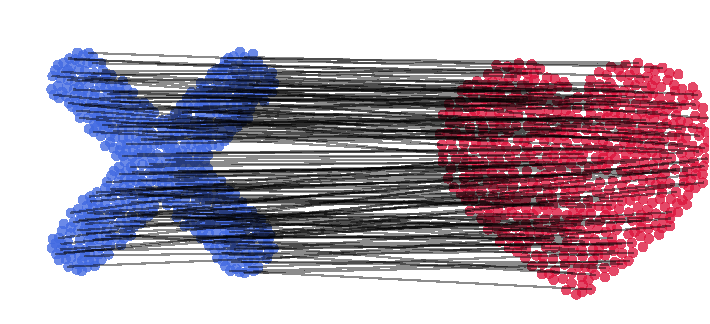
\includegraphics[width=.47\linewidth]{figures/fig-static/cross-heart_static_pairing_p1.pdf}
&
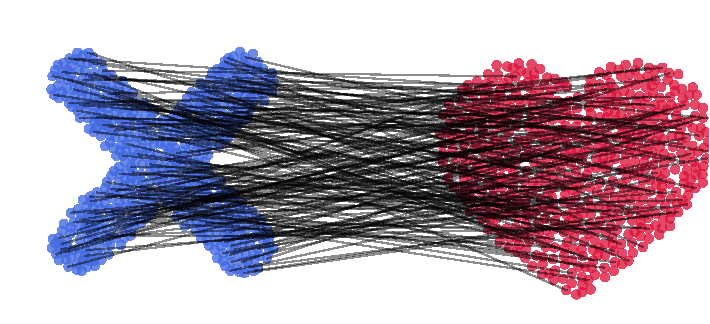
\includegraphics[width=.47\linewidth]{figures/fig-static/cross-heart_static_pairing_pinf.pdf}
\\[-.2em]
\small Cross to heart, $p=1$
&
\small Cross to heart, $p=\infty$
\\[.5em]
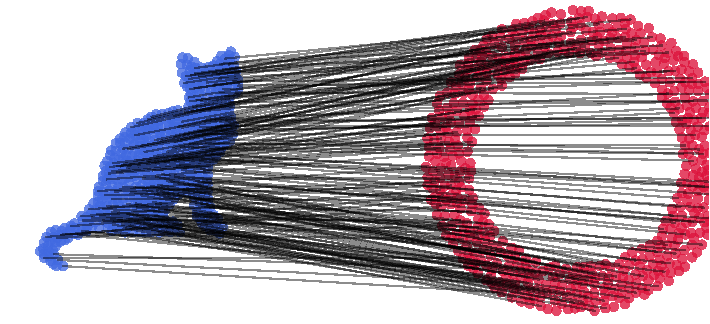
\includegraphics[width=.47\linewidth]{figures/fig-static/cat-annulus_static_pairing_p1.pdf}
&
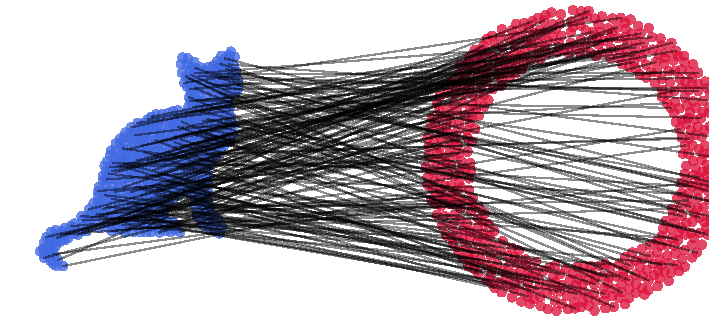
\includegraphics[width=.47\linewidth]{figures/fig-static/cat-annulus_static_pairing_pinf.pdf}
\\[-.2em]
\small Cat to annulus, $p=1$
&
\small Cat to annulus, $p=\infty$
\end{tabular}
\caption{Additional static Spectral Wasserstein couplings. Only a subsample of matching segments is displayed.}
\label{fig:extra-static-pairs}
\end{figure}

Figure~\ref{fig:extra-static-interp} displays the corresponding displacement-interpolation density snapshots, using the same optimal couplings as in Figure~\ref{fig:extra-static-pairs}.
\begin{figure}[!t]
\centering
\resizebox{\linewidth}{!}{%
\begin{tabular}{@{}cccccccccc@{}}
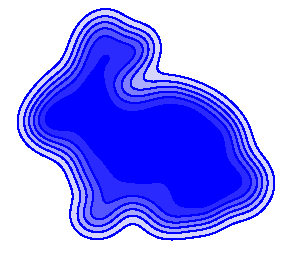
\includegraphics[width=.098\linewidth]{figures/fig-dynamics/bunny-trefle_static_interp_p1_t0.pdf}
&
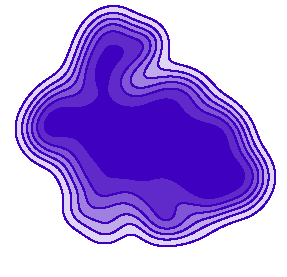
\includegraphics[width=.098\linewidth]{figures/fig-dynamics/bunny-trefle_static_interp_p1_t1.pdf}
&
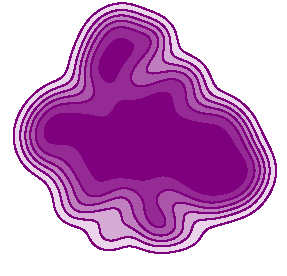
\includegraphics[width=.098\linewidth]{figures/fig-dynamics/bunny-trefle_static_interp_p1_t2.pdf}
&
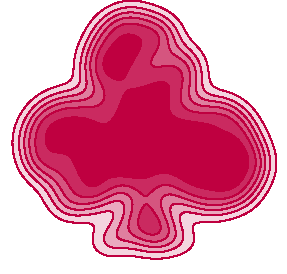
\includegraphics[width=.098\linewidth]{figures/fig-dynamics/bunny-trefle_static_interp_p1_t3.pdf}
&
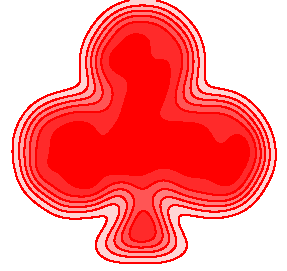
\includegraphics[width=.098\linewidth]{figures/fig-dynamics/bunny-trefle_static_interp_p1_t4.pdf}
&
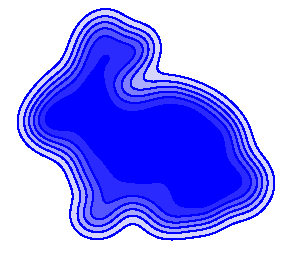
\includegraphics[width=.098\linewidth]{figures/fig-dynamics/bunny-trefle_static_interp_pinf_t0.pdf}
&
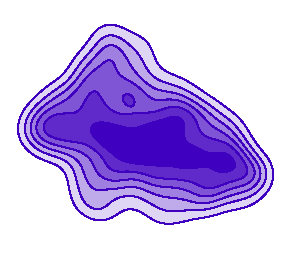
\includegraphics[width=.098\linewidth]{figures/fig-dynamics/bunny-trefle_static_interp_pinf_t1.pdf}
&
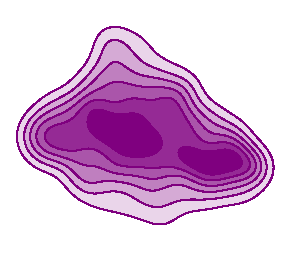
\includegraphics[width=.098\linewidth]{figures/fig-dynamics/bunny-trefle_static_interp_pinf_t2.pdf}
&
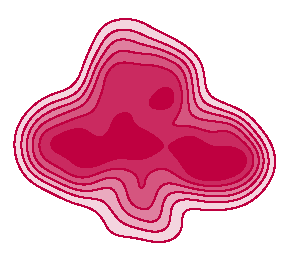
\includegraphics[width=.098\linewidth]{figures/fig-dynamics/bunny-trefle_static_interp_pinf_t3.pdf}
&
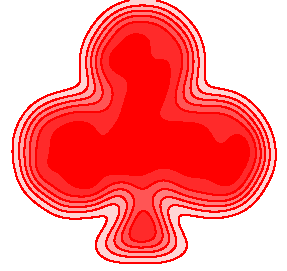
\includegraphics[width=.098\linewidth]{figures/fig-dynamics/bunny-trefle_static_interp_pinf_t4.pdf}
\\[-.2em]
& & \small $p=1$ & & & & & \small $p=\infty$ & &
\\[.35em]
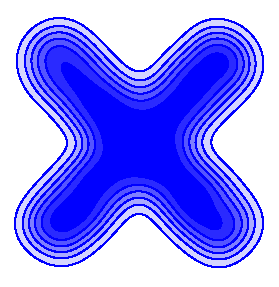
\includegraphics[width=.098\linewidth]{figures/fig-dynamics/cross-heart_static_interp_p1_t0.pdf}
&
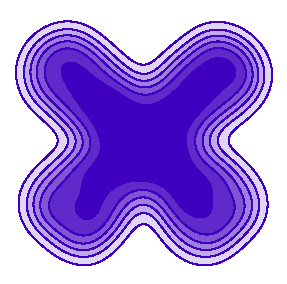
\includegraphics[width=.098\linewidth]{figures/fig-dynamics/cross-heart_static_interp_p1_t1.pdf}
&
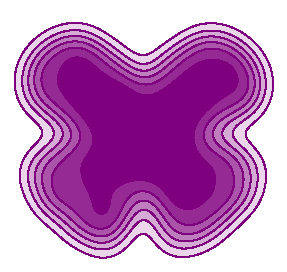
\includegraphics[width=.098\linewidth]{figures/fig-dynamics/cross-heart_static_interp_p1_t2.pdf}
&
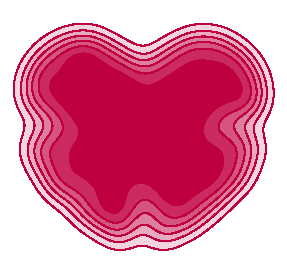
\includegraphics[width=.098\linewidth]{figures/fig-dynamics/cross-heart_static_interp_p1_t3.pdf}
&

\includegraphics[width=.098\linewidth]{figures/fig-dynamics/cross-heart_static_interp_p1_t4.pdf}
&
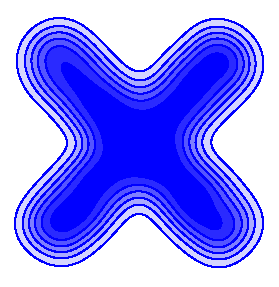
\includegraphics[width=.098\linewidth]{figures/fig-dynamics/cross-heart_static_interp_pinf_t0.pdf}
&
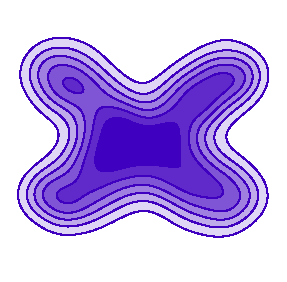
\includegraphics[width=.098\linewidth]{figures/fig-dynamics/cross-heart_static_interp_pinf_t1.pdf}
&
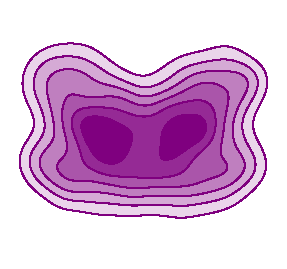
\includegraphics[width=.098\linewidth]{figures/fig-dynamics/cross-heart_static_interp_pinf_t2.pdf}
&
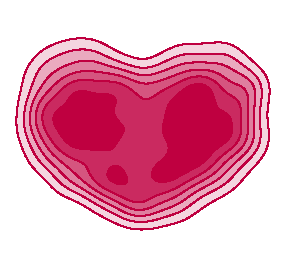
\includegraphics[width=.098\linewidth]{figures/fig-dynamics/cross-heart_static_interp_pinf_t3.pdf}
&

\includegraphics[width=.098\linewidth]{figures/fig-dynamics/cross-heart_static_interp_pinf_t4.pdf}
\\[-.2em]
& & \small $p=1$ & & & & & \small $p=\infty$ & &
\\[.35em]
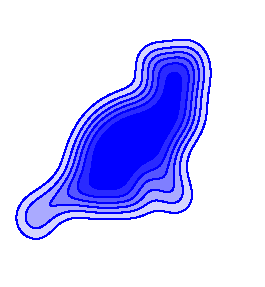
\includegraphics[width=.098\linewidth]{figures/fig-dynamics/cat-annulus_static_interp_p1_t0.pdf}
&
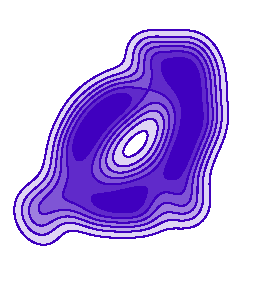
\includegraphics[width=.098\linewidth]{figures/fig-dynamics/cat-annulus_static_interp_p1_t1.pdf}
&
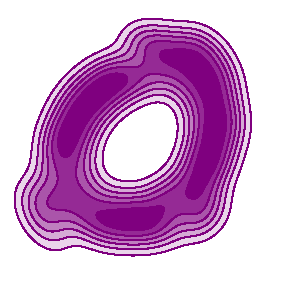
\includegraphics[width=.098\linewidth]{figures/fig-dynamics/cat-annulus_static_interp_p1_t2.pdf}
&
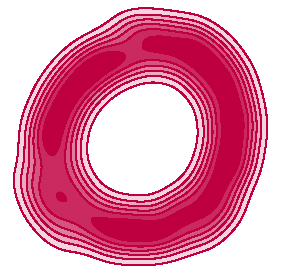
\includegraphics[width=.098\linewidth]{figures/fig-dynamics/cat-annulus_static_interp_p1_t3.pdf}
&
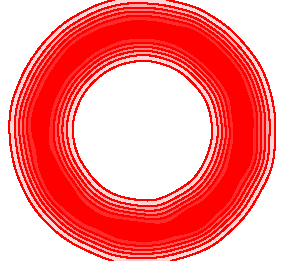
\includegraphics[width=.098\linewidth]{figures/fig-dynamics/cat-annulus_static_interp_p1_t4.pdf}
&
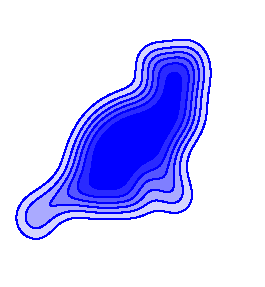
\includegraphics[width=.098\linewidth]{figures/fig-dynamics/cat-annulus_static_interp_pinf_t0.pdf}
&
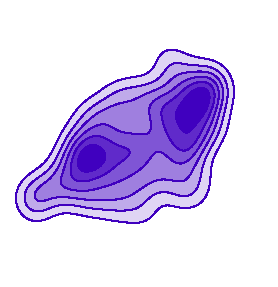
\includegraphics[width=.098\linewidth]{figures/fig-dynamics/cat-annulus_static_interp_pinf_t1.pdf}
&
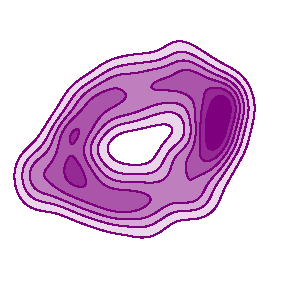
\includegraphics[width=.098\linewidth]{figures/fig-dynamics/cat-annulus_static_interp_pinf_t2.pdf}
&
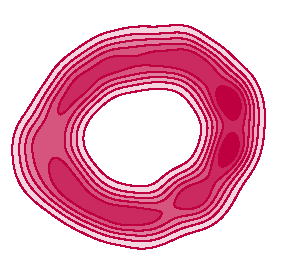
\includegraphics[width=.098\linewidth]{figures/fig-dynamics/cat-annulus_static_interp_pinf_t3.pdf}
&
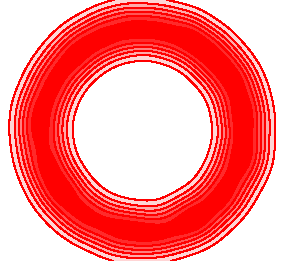
\includegraphics[width=.098\linewidth]{figures/fig-dynamics/cat-annulus_static_interp_pinf_t4.pdf}
\\[-.2em]
& & \small $p=1$ & & & & & \small $p=\infty$ & &
\end{tabular}
}
\caption{Additional displacement-interpolation density snapshots for the same shape pairs as Figure~\ref{fig:extra-static-pairs}.}
\label{fig:extra-static-interp}
\end{figure}

\FloatBarrier

\section{Geodesic Convexity}
\label{app:convexity}
This section studies one of the basic structural notions behind metric gradient flows, namely geodesic convexity, for the Spectral Wasserstein geometries introduced above. Geodesic convexity is desirable because it supports stability and global convergence statements \citep{AmbrosioGigliSavare2008}, but for many machine-learning objectives it is arguably too strong, so here it is used as a structural benchmark rather than as a blanket modeling assumption.
\subsection{Definition and General Setup}
This subsection recalls the relevant notion of convexity along Spectral Wasserstein geodesics and explains why it matters for the variational analysis of the flow.
When one studies gradient flows in metric spaces, geodesic convexity plays the same role as ordinary convexity in Euclidean optimization: it governs uniqueness, stability, and the variational structure of the dynamics. Since Corollary~\ref{cor:geodesic} shows that $\Wg$-geodesics are displacement interpolations associated with optimal couplings, the corresponding convexity inequalities can be tested directly along Euclidean segments.

The next definition fixes the notion used in the remainder of this section.
\begin{definition}[Geodesic convexity]
\label{def:geoconvex}
A functional $F:\cP_2(\R^d)\to(-\infty,+\infty]$ is called $\kappa$-geodesically convex for $\Wg$ if along every constant-speed $\Wg$-geodesic $(\mu_t)_{t\in[0,1]}$ one has
$$
F(\mu_t)
\le
(1-t)F(\mu_0)+tF(\mu_1)
-\frac{\kappa}{2}t(1-t)\Wg(\mu_0,\mu_1)^2.
$$
\end{definition}

\subsection{Linear Functionals}
This subsection shows that for linear functionals the qualitative and quantitative convexity criteria reduce to explicit pointwise conditions on the integrand.
For a Borel function $h:\R^d\to\R$, define the linear functional
$$
F_h(\mu)\coloneqq \int_{\R^d} h(x)\,d\mu(x).
$$
Because $\Wg$-geodesics are still given by affine interpolation in space, the convexity question for $F_h$ is especially transparent.

The next theorem gives the exact criterion.
\begin{theorem}[Linear functionals]
\label{thm:linearconvex}
Assume $\gamma$ is monotone and let $\cK$ be a convex compact PSD representing set for $\gamma$ as in Proposition~\ref{prop:psdpolar}.
\begin{enumerate}
\item The functional $F_h$ is geodesically convex for $\Wg$ if and only if $h$ is convex on $\R^d$.
\item If in addition $h\in C^2(\R^d)$ and $\kappa\ge0$, then $F_h$ is $\kappa$-geodesically convex for $\Wg$ if and only if
$$
\nabla^2 h(z)\succeq \kappa Q
\qquad
\text{for every }z\in\R^d,\ Q\in\cK.
$$
Equivalently,
$$
\xi^\top \nabla^2 h(z)\,\xi
\ge
\kappa\max_{Q\in\cK}\xi^\top Q\,\xi
\qquad
\text{for every }z,\xi\in\R^d.
$$
For $\kappa<0$, this displayed scalar reformulation with a maximum is not equivalent to the matrix inequality; multiplication by the negative scalar reverses the extremum, so the corresponding pointwise scalar condition would involve $\min_{Q\in\cK}\xi^\top Q\xi$. No equivalence for negative $\kappa$ is asserted here.
\end{enumerate}
\end{theorem}

\begin{proof}
Assume first that $h$ is convex and let
$$
\mu_t=((1-t)x+ty)_\#\pi_*
$$
be any constant-speed $\Wg$-geodesic. Then
$$
F_h(\mu_t)
=
\int h((1-t)x+ty)\,d\pi_*(x,y).
$$
By the convexity of $h$,
$$
h((1-t)x+ty)\le (1-t)h(x)+th(y),
$$
and integrating yields geodesic convexity of $F_h$.

Conversely, if $F_h$ is geodesically convex, apply the definition to Dirac masses $\mu_0=\delta_x$ and $\mu_1=\delta_y$. The unique geodesic is
$$
\mu_t=\delta_{(1-t)x+ty},
$$
so
$$
h((1-t)x+ty)=F_h(\mu_t)\le (1-t)h(x)+th(y),
$$
which proves convexity of $h$.

Assume now that $h\in C^2$ and that
$$
\nabla^2 h(z)\succeq \kappa Q
\qquad
\text{for every }z\in\R^d,\ Q\in\cK.
$$
Let
$$
\mu_t=((1-t)x+ty)_\#\pi_*
$$
be any constant-speed $\Wg$-geodesic, write $z_t=(1-t)x+ty$ and $\Delta=y-x$. Differentiating under the integral sign gives
$$
\frac{d^2}{dt^2}F_h(\mu_t)
=
\int \Delta^\top \nabla^2 h(z_t)\Delta\,d\pi_*(x,y).
$$
For every $Q\in\cK$ this implies
$$
\frac{d^2}{dt^2}F_h(\mu_t)
\ge
\kappa\int \Delta^\top Q\Delta\,d\pi_*(x,y).
$$
Since $\kappa\ge0$, taking the maximum over $Q\in\cK$ yields
$$
\frac{d^2}{dt^2}F_h(\mu_t)
\ge
\kappa\gamma\!\left(\int \Delta\Delta^\top\,d\pi_*(x,y)\right)
=
\kappa\Wg(\mu_0,\mu_1)^2.
$$
Integrating twice in $t$ gives the $\kappa$-geodesic convexity estimate.

Conversely, assume $F_h$ is $\kappa$-geodesically convex. Testing the definition on the Dirac geodesic between $\delta_z$ and $\delta_{z+\xi}$ gives
$$
h(z+t\xi)
\le
(1-t)h(z)+th(z+\xi)
-\frac{\kappa}{2}t(1-t)\gamma(\xi\xi^\top).
$$
Differentiating at second order in $t$ yields
$$
\xi^\top \nabla^2 h(z)\,\xi
\ge
\kappa\gamma(\xi\xi^\top)
=
\kappa\max_{Q\in\cK}\xi^\top Q\,\xi.
$$
Because $\kappa\ge0$, this scalar inequality is equivalent to the matrix inequality
$$
\nabla^2 h(z)\succeq \kappa Q
\qquad
\text{for every }Q\in\cK.
$$
\end{proof}

The next remark interprets the condition of Theorem~\ref{thm:linearconvex} for the Schatten family.
\begin{remark}[Schatten norms]
For the Schatten geometries used throughout the paper and for $\kappa\ge0$, the condition
$$
\nabla^2 h(z)\succeq \kappa Q
\qquad
\text{for every }Q\in\cK
$$
is equivalent to
$$
\nabla^2 h(z)\succeq \kappa \Id.
$$
Indeed, for $p=1$ we may choose $\cK=\{\Id\}$. For $1<p\le \infty$, a convenient choice is
$$
\cK=\{Q\succeq 0:\ \norm{Q}_{S_q}\le 1\},
\qquad
q=\frac{p}{p-1},
$$
with the usual interpretation $q=1$ when $p=\infty$. Under the standing condition $\kappa\ge0$ in Theorem~\ref{thm:linearconvex}, every such $Q$ satisfies $Q\preceq\Id$, and every rank-one projector belongs to $\cK$; hence the condition is equivalent to $\nabla^2h(z)\succeq\kappa\Id$, exactly as in the classical $\Wtwo$ geometry. For negative $\kappa$, this simplification is not asserted.
\end{remark}

\subsection{Relative Entropy}

This subsection examines the geodesic convexity of relative entropy, which is a fundamental nonlinear example underlying diffusion-type gradient flows.
%
Section~\ref{sec:relative-entropy-gaussians} treats in detail the case of a Gaussian target $\nu$, for which Gaussians are stable, and boils down to the study of an ODE. 
%
Let
$$
d\nu(x)=Z^{-1}e^{-V(x)}\,dx,
\qquad
V\in C^2(\R^d),
$$
and define the relative entropy
$$
\operatorname{Ent}_\nu(\mu)\coloneqq 
\begin{cases}
\displaystyle \int \log\!\left(\frac{d\mu}{d\nu}\right)\,d\mu, & \mu\ll \nu,\\[0.6em]
+\infty, & \text{otherwise}.
\end{cases}
$$
The trace case is the classical displacement-convexity theory of entropy. For general spectral geometries the same argument works only when the active quadratic costs remain uniformly elliptic, and otherwise one only gets a weaker statement by approximation.

The next theorem records the full all-geodesics result in the uniformly elliptic regime.
\begin{theorem}[Full entropy convexity under uniform ellipticity]
\label{thm:entropyfull}
Assume $\gamma$ is monotone and that $\cK$ can be chosen so that
$$
\cK\subset \Sppd.
$$
Assume moreover that
$$
\nabla^2 V(x)\succeq \kappa Q
\qquad
\text{for every }x\in\R^d,\ Q\in\cK.
$$
Then $\operatorname{Ent}_\nu$ is $\kappa$-geodesically convex on $(\cP_2(\R^d),\Wg)$.
\end{theorem}

\begin{proof}
Let
$$
\mu_t=((1-t)x+ty)_\#\pi_*
$$
be any constant-speed $\Wg$-geodesic, and set
$$
S_*=\int (y-x)(y-x)^\top\,d\pi_*(x,y).
$$
Choose $Q_*\in\cK$ such that
$$
\tr(Q_*S_*)=\gamma(S_*)=\Wg(\mu_0,\mu_1)^2.
$$
By Theorem~\ref{thm:minmax}, the same coupling $\pi_*$ is optimal for the quadratic cost
$$
c_{Q_*}(x,y)=(y-x)^\top Q_*(y-x),
$$
and
$$
\WQ{Q_*}(\mu_0,\mu_1)^2=\Wg(\mu_0,\mu_1)^2.
$$

Since $Q_*$ is positive definite, let $L=Q_*^{1/2}$ and define
$$
\widetilde\mu_i=L_\#\mu_i,
\qquad
\widetilde\nu=L_\#\nu,
\qquad
\widetilde\pi_*=(L,L)_\#\pi_*.
$$
Then $\widetilde\pi_*$ is optimal for the Euclidean quadratic cost between $\widetilde\mu_0$ and $\widetilde\mu_1$, hence
$$
\widetilde\mu_t=((1-t)z_0+t z_1)_\#\widetilde\pi_*
$$
is a $\Wtwo$-geodesic and
$$
\Wtwo(\widetilde\mu_0,\widetilde\mu_1)^2=\Wg(\mu_0,\mu_1)^2.
$$

The reference measure $\widetilde\nu$ has density
$$
d\widetilde\nu(z)=\widetilde Z^{-1}e^{-\widetilde V(z)}\,dz,
\qquad
\widetilde V(z)=V(L^{-1}z)+\text{constant},
$$
so
$$
\nabla^2\widetilde V(z)=L^{-1}\nabla^2V(L^{-1}z)L^{-1}.
$$
Because $Q_*\in\cK$, the curvature assumption gives
$$
\nabla^2V(x)\succeq \kappa Q_*=\kappa L^2,
$$
hence
$$
\nabla^2\widetilde V(z)\succeq \kappa \Id.
$$
The classical entropy convexity theorem for $\Wtwo$ therefore yields
$$
\operatorname{Ent}_{\widetilde\nu}(\widetilde\mu_t)
\le
(1-t)\operatorname{Ent}_{\widetilde\nu}(\widetilde\mu_0)
+t\operatorname{Ent}_{\widetilde\nu}(\widetilde\mu_1)
-\frac{\kappa}{2}t(1-t)\Wtwo(\widetilde\mu_0,\widetilde\mu_1)^2.
$$
Finally, relative entropy is invariant under the invertible change of variables $L$, so
$$
\operatorname{Ent}_{\widetilde\nu}(\widetilde\mu_t)=\operatorname{Ent}_\nu(\mu_t),
$$
and similarly at the endpoints. This gives the result.
\end{proof}

The next theorem explains what remains true in the more relevant but singular regime where the condition $\cK\subset \Sppd$ fails. This lack of ellipticity is precisely what happens for Schatten-$p$ geometries with $p>1$, because the corresponding representing sets contain singular matrices, but one still retains a weaker geodesic-convexity statement by approximation.
\begin{theorem}[Weak entropy convexity]
\label{thm:entropyweak}
Assume $\gamma$ is monotone, that $\cK\subset \mathbb S_+^d$ is convex compact, and that
$$
\cK\cap \Sppd\neq \varnothing.
$$
Assume moreover that
$$
\nabla^2V(x)\succeq \kappa Q
\qquad
\text{for every }x\in\R^d,\ Q\in\cK.
$$
Then for every $\mu_0,\mu_1\in\cP_2(\R^d)$ there exists at least one constant-speed $\Wg$-geodesic $(\mu_t)_{t\in[0,1]}$ from $\mu_0$ to $\mu_1$ such that
$$
\operatorname{Ent}_\nu(\mu_t)
\le
(1-t)\operatorname{Ent}_\nu(\mu_0)+t\operatorname{Ent}_\nu(\mu_1)
-\frac{\kappa}{2}t(1-t)\Wg(\mu_0,\mu_1)^2.
$$
\end{theorem}

\begin{proof}
Choose $Q_0\in\cK\cap \Sppd$ and define
$$
\mathcal K_{\gamma,\varepsilon}\coloneqq (1-\varepsilon)\cK+\varepsilon Q_0,
\qquad
\varepsilon\in(0,1).
$$
Then every element of $\mathcal K_{\gamma,\varepsilon}$ is positive definite. Let $\gamma_\varepsilon$ be the support function of $\mathcal K_{\gamma,\varepsilon}$, namely
$$
\gamma_\varepsilon(S)=\max_{Q\in\mathcal K_{\gamma,\varepsilon}}\tr(QS)
=(1-\varepsilon)\gamma(S)+\varepsilon\tr(Q_0S).
$$
Hence
$$
(1-\varepsilon)\gamma(S)\le \gamma_\varepsilon(S)\le \gamma(S)
$$
for all $S\succeq 0$, and therefore
$$
(1-\varepsilon)\Wg(\mu_0,\mu_1)^2
\le
\mathsf W_{\gamma_\varepsilon}(\mu_0,\mu_1)^2
\le
\Wg(\mu_0,\mu_1)^2.
$$

By Theorem~\ref{thm:entropyfull}, each regularized geometry has full entropy convexity. Choose an optimal coupling $\pi_\varepsilon$ for $\mathsf W_{\gamma_\varepsilon}$ and set
$$
\mu_t^\varepsilon=((1-t)x+ty)_\#\pi_\varepsilon.
$$
Then
$$
\operatorname{Ent}_\nu(\mu_t^\varepsilon)
\le
(1-t)\operatorname{Ent}_\nu(\mu_0)+t\operatorname{Ent}_\nu(\mu_1)
-\frac{\kappa}{2}t(1-t)\mathsf W_{\gamma_\varepsilon}(\mu_0,\mu_1)^2.
$$
By compactness of couplings, one may extract a subsequence $\pi_{\varepsilon_n}\rightharpoonup \pi_*$. Setting
$$
\mu_t=((1-t)x+ty)_\#\pi_*,
$$
the lower semicontinuity of relative entropy and the convergence
$$
\mathsf W_{\gamma_{\varepsilon_n}}(\mu_0,\mu_1)^2\to \Wg(\mu_0,\mu_1)^2
$$
yield the claimed inequality along the limit geodesic. The limit coupling $\pi_*$ is $\Wg$-optimal by continuity of the displacement covariance and of the support functions on trace-bounded sets.
\end{proof}

The next proposition shows that, in the operator case, full geodesic convexity of relative entropy fails in a very concrete way.
\begin{proposition}[Operator-norm counterexample]
\label{prop:entropy-counterexample}
Let $\gamma(S)=\lambda_{\max}(S)$ on $\mathbb S_+^2$, and let
$$
d\nu(x)=\frac{1}{2\pi}e^{-|x|^2/2}\,dx.
$$
Then $\operatorname{Ent}_\nu$ is not geodesically convex on $(\cP_2(\R^2),\mathsf W_{\gamma})$.
\end{proposition}

\begin{proof}
Fix parameters $L>0$ and $a>0$ such that
$$
\frac{4a^2}{3}\le L^2.
$$
Set
$$
R_0=[0,1]\times[-a,a],
\qquad
R_1=[L,L+1]\times[-a,a],
$$
and let
$$
\mu_i=\frac{1}{2a}\mathbf 1_{R_i}\,dx,
\qquad i=0,1.
$$
Both endpoints are absolutely continuous with bounded support, hence satisfy
$$
\operatorname{Ent}_\nu(\mu_0)<+\infty,
\qquad
\operatorname{Ent}_\nu(\mu_1)<+\infty.
$$

For any coupling $\pi$ between $\mu_0$ and $\mu_1$, define
$$
S_\pi=\int (y-x)(y-x)^\top\,d\pi(x,y).
$$
Then
$$
\lambda_{\max}(S_\pi)\ge e_1^\top S_\pi e_1
=\int (y_1-x_1)^2\,d\pi(x,y)
\ge
\left(\int (y_1-x_1)\,d\pi(x,y)\right)^2
=L^2.
$$
Hence every admissible coupling has operator cost at least $L^2$.

The translation map
$$
T(x_1,x_2)=(x_1+L,x_2)
$$
pushes $\mu_0$ to $\mu_1$ and has covariance
$$
S_T=\diag(L^2,0),
$$
so $\mathsf W_{\gamma}(\mu_0,\mu_1)^2=L^2$.

Now consider the reflected transport
$$
R(x_1,x_2)=(x_1+L,-x_2).
$$
It also pushes $\mu_0$ to $\mu_1$ because the second marginal of $\mu_0$ is symmetric on $[-a,a]$. Its displacement is
$$
R(x)-x=(L,-2x_2),
$$
hence
$$
S_R=\diag\!\left(L^2,\frac{4a^2}{3}\right).
$$
By the choice of $a$,
$$
\lambda_{\max}(S_R)=L^2,
$$
so the coupling induced by $R$ is again optimal for $\mathsf W_{\gamma}$.

Consider the corresponding constant-speed geodesic
$$
\mu_t=((1-t)\Id+tR)_\#\mu_0.
$$
At time $t=\frac12$ one gets
$$
\mu_{1/2}
=
\left(x_1+\frac{L}{2},0\right)_\#\mu_0,
$$
which is the uniform measure on the horizontal segment
$$
\left[\frac{L}{2},\frac{L}{2}+1\right]\times\{0\}.
$$
Therefore $\mu_{1/2}$ is singular with respect to Lebesgue measure, hence also singular with respect to $\nu$, and thus
$$
\operatorname{Ent}_\nu(\mu_{1/2})=+\infty.
$$
So along this optimal $\mathsf W_{\gamma}$-geodesic the endpoints have finite entropy while the midpoint has infinite entropy, which rules out geodesic convexity.
\end{proof}

The next remark explains why Proposition~\ref{prop:entropy-counterexample} does not contradict Theorem~\ref{thm:entropyweak}.
\begin{remark}[Why there is no contradiction]
Theorem~\ref{thm:entropyweak} is an existence statement: for each pair of endpoints it guarantees at least one $\Wg$-geodesic along which the entropy inequality holds. Proposition~\ref{prop:entropy-counterexample} proves something different, namely that in the operator geometry there also exist optimal geodesics along which the entropy blows up at an interior time. So the counterexample rules out full all-geodesics convexity, but it does not preclude the existence of another optimal geodesic selected by the approximation argument in Theorem~\ref{thm:entropyweak} and enjoying the convexity estimate.
\end{remark}

The following remark explains the scope of the entropy results for the Schatten family.
\begin{remark}[Schatten norms]
The full theorem applies to the trace case $p=1$, where one may choose $\cK=\{\Id\}$ and recover the classical $\Wtwo$ displacement-convexity theory. For every Schatten geometry with $1<p\le \infty$, the natural representing sets contain singular matrices, so the uniformly elliptic argument above does not apply directly. Theorem~\ref{thm:entropyweak} nevertheless yields a weak geodesic-convexity statement as soon as $\cK$ contains one positive definite matrix, which is the case for the standard Schatten choices.
\end{remark}


%%%

\subsection{Relative-entropy flows over Gaussians}
\label{sec:relative-entropy-gaussians}

\newcommand{\KL}{\mathrm{KL}}

The $\Wtwo$-gradient flow of the relative entropy
$\operatorname{Ent}_\nu(\mu) = \KL(\mu\,|\,\nu)$ is the Langevin/Fokker--Planck equation, whose stochastic
single-particle realization is the overdamped Langevin diffusion. This makes
it a basic tool for sampling. We now describe what happens for the spectral
Schatten geometries. For $p>1$, the resulting evolution is still explicit on
Gaussian measures, but the PDE is nonlocal: its velocity depends on global
statistics of the current law, and therefore cannot be represented by an
autonomous single-particle SDE with coefficients depending only on the
particle position.

\begin{proposition}[Gaussian KL flow for Schatten geometries]
\label{prop:gaussian-kl-schatten-flow}
Let $\nu=\mathcal N(\bar m,\bar\Sigma)$ with $\bar\Sigma\succ0$, and consider
$\mathcal F(\mu)=\KL(\mu\,|\,\nu)$. The Shatten-$p$ flow solution $\mu_t$ of $\mathcal{F}$ is Gaussian $\mu_t = \mathcal{N}(m_t,\Sigma_t)$. 
%
Define the classical $p=1$ Gaussian velocity by
$\dot m_t^{(1)}\coloneqq-\bar\Sigma^{-1}(m_t-\bar m)$ and
$\dot\Sigma_t^{(1)}\coloneqq
2I-\bar\Sigma^{-1}\Sigma_t-\Sigma_t\bar\Sigma^{-1}$.
Then the trace geometry $p=1$ satisfies
$\dot m_t=\dot m_t^{(1)}$ and $\dot\Sigma_t=\dot\Sigma_t^{(1)}$.

For a general Schatten geometry $p\in[1,\infty]$, set
$q\coloneqq 2p/(2p-1)$, with the convention $q=1$ when $p=\infty$, and define
\[
    F_t
    \coloneqq
    (\bar\Sigma^{-1}-\Sigma_t^{-1})\Sigma_t
    (\bar\Sigma^{-1}-\Sigma_t^{-1})
    +
    \bar\Sigma^{-1}(m_t-\bar m)(m_t-\bar m)^\top\bar\Sigma^{-1}.
\]
Assume $F_t\succ0$ and define
\[
    \mathcal N_t^q\coloneqq \tr(F_t^{q/2}),
    \qquad
    P_{p,t}\coloneqq \mathcal N_t^{2-q}F_t^{q/2-1}.
\]
Then the Schatten-$p$ Gaussian KL flow is
\[
    \dot m_t=P_{p,t}\dot m_t^{(1)},
    \qquad
    \dot\Sigma_t
    =
    \frac12\left(
        P_{p,t}\dot\Sigma_t^{(1)}
        +
        \dot\Sigma_t^{(1)}P_{p,t}
    \right).
\]
In particular, for $p=1$, one has $q=2$, $P_{1,t}=I$, and the classical
Langevin covariance equation is recovered. For $p=\infty$, one has
\[
    P_{\infty,t}=\tr(F_t^{1/2})F_t^{-1/2}.
\]
\end{proposition}

\begin{proof}
For $\mu_t=\mathcal N(m_t,\Sigma_t)$ and
$\nu=\mathcal N(\bar m,\bar\Sigma)$, the first variation of
$\KL(\mu\,|\,\nu)$ has Wasserstein gradient
\[
    g_t(x)
    =
    \nabla_x\log\frac{d\mu_t}{d\nu}(x)
    =
    (\bar\Sigma^{-1}-\Sigma_t^{-1})(x-m_t)
    +
    \bar\Sigma^{-1}(m_t-\bar m).
\]
Thus $g_t$ is affine. Set
$H_t\coloneqq\bar\Sigma^{-1}-\Sigma_t^{-1}$ and
$b_t\coloneqq\bar\Sigma^{-1}(m_t-\bar m)$, so that
$g_t(x)=H_t(x-m_t)+b_t$. Since
$\int(x-m_t)\,d\mu_t(x)=0$ and
$\int(x-m_t)(x-m_t)^\top\,d\mu_t(x)=\Sigma_t$, the covariance matrix of
$g_t$ is exactly
\[
    \int g_t(x)g_t(x)^\top\,d\mu_t(x)
    =
    H_t\Sigma_tH_t+b_tb_t^\top
    =
    F_t.
\]

For the Schatten geometry associated with $p$, the Measure-LMO gives the
velocity
\[
    v_t(x)
    =
    -P_{p,t}g_t(x),
    \qquad
    P_{p,t}=\mathcal N_t^{2-q}F_t^{q/2-1},
    \qquad
    \mathcal N_t^q=\tr(F_t^{q/2}).
\]
This formula is the Schatten duality map applied to the vector field $g_t$.
Because $g_t$ is affine and $P_{p,t}$ is independent of $x$, the velocity
$v_t$ is affine in $x$. Therefore the continuity equation
$\partial_t\mu_t+\divv(\mu_t v_t)=0$ preserves the Gaussian family.

We now compute the induced ODE on mean and covariance. Since
$v_t(x)=-P_{p,t}H_t(x-m_t)-P_{p,t}b_t$, the mean satisfies
\[
    \dot m_t
    =
    \int v_t(x)\,d\mu_t(x)
    =
    -P_{p,t}b_t.
\]
But
$b_t=\bar\Sigma^{-1}(m_t-\bar m)$, hence
$-b_t=\dot m_t^{(1)}$. Therefore
$\dot m_t=P_{p,t}\dot m_t^{(1)}$.

For the covariance, using
$\dot\Sigma_t=\int \bigl(v_t(x)(x-m_t)^\top
+(x-m_t)v_t(x)^\top\bigr)\,d\mu_t(x)$, we obtain
\[
    \dot\Sigma_t
    =
    -P_{p,t}H_t\Sigma_t-\Sigma_tH_tP_{p,t}.
\]
On the other hand,
\[
    \dot\Sigma_t^{(1)}
    =
    2I-\bar\Sigma^{-1}\Sigma_t-\Sigma_t\bar\Sigma^{-1}.
\]
Since $H_t=\bar\Sigma^{-1}-\Sigma_t^{-1}$ and both
$\bar\Sigma^{-1}$ and $\Sigma_t^{-1}$ are symmetric,
\[
    -H_t\Sigma_t
    =
    I-\bar\Sigma^{-1}\Sigma_t,
    \qquad
    -\Sigma_tH_t
    =
    I-\Sigma_t\bar\Sigma^{-1}.
\]
Therefore
\[
    -P_{p,t}H_t\Sigma_t-\Sigma_tH_tP_{p,t}
    =
    P_{p,t}(I-\bar\Sigma^{-1}\Sigma_t)
    +
    (I-\Sigma_t\bar\Sigma^{-1})P_{p,t}.
\]
When $P_{p,t}$ commutes with the symmetric part of the classical covariance
velocity, this is exactly
$\frac12(P_{p,t}\dot\Sigma_t^{(1)}
+\dot\Sigma_t^{(1)}P_{p,t})$. More generally, the correct intrinsic
twisted form is
\[
    \dot\Sigma_t
    =
    P_{p,t}(I-\bar\Sigma^{-1}\Sigma_t)
    +
    (I-\Sigma_t\bar\Sigma^{-1})P_{p,t}.
\]
In the common commuting setting, or whenever
$\bar\Sigma^{-1}\Sigma_t=\Sigma_t\bar\Sigma^{-1}$, this reduces to the
displayed symmetrized formula in the statement.

Finally, for $p=1$ one has $q=2$, hence
$\mathcal N_t^{2-q}=1$ and $F_t^{q/2-1}=I$, so $P_{1,t}=I$. The equations
therefore reduce to
$\dot m_t=-\bar\Sigma^{-1}(m_t-\bar m)$ and
$\dot\Sigma_t=2I-\bar\Sigma^{-1}\Sigma_t-\Sigma_t\bar\Sigma^{-1}$, which is
the Gaussian restriction of the classical Langevin/Fokker--Planck flow. For
$p=\infty$, $q=1$, giving
$P_{\infty,t}=\tr(F_t^{1/2})F_t^{-1/2}$.
\end{proof}



%%%

\section{Positively \texorpdfstring{$2$}{2}-Homogeneous Case and a Generalized Unbalanced Geometry}
\label{app:homogeneous}
This section continues the two-layer mean-field discussion of Section~\ref{sec:mlp-meanfield} in the positively two-homogeneous case. The point is that such models reduce the ambient transport problem to an unbalanced transport problem on the sphere, and this section explains how the spherical dynamics inherits a spectral action from the ambient flow.
Let
$$
\MF(\mu)=R\!\left(\int_{\R^d}\Phi(x)\,d\mu(x)\right),
\qquad
\Phi(\lambda x)=\lambda^2\Phi(x).
$$
Writing $x=r\omega$ with $\omega\in\Sd$, define the weighted spherical projection
$$
\int_{\Sd}\psi(\omega)\,d\Pi_2(\mu)(\omega)
\coloneqq 
\int_{\R^d}\abs{x}^2\psi\!\left(\frac{x}{\abs{x}}\right)\,d\mu(x).
$$
The first point is that two-homogeneous models only depend on this weighted spherical projection.
\begin{proposition}[Exact quotient]
\label{prop:quotient}
There exists a functional $\overline f$ on $\cM_+(\Sd)$ such that
$$
\MF(\mu)=\overline f(\Pi_2(\mu)).
$$
\end{proposition}

\begin{proof}
The homogeneity identity $\Phi(r\omega)=r^2\Phi(\omega)$ immediately gives
$$
\int_{\R^d}\Phi(x)\,d\mu(x)
=
\int_{\Sd}\Phi(\omega)\,d\Pi_2(\mu)(\omega),
$$
which defines $\overline f$.
\end{proof}

The second point is that the ambient normalized velocity splits into radial and tangential parts on the sphere. If a vector field $v$ is $1$-homogeneous, namely $v(\lambda x)=\lambda v(x)$ for every $\lambda>0$, then for every $x=r\omega\neq 0$ it can be written uniquely as
$$
v(r\omega)=r\bigl(b(\omega)\omega+\tau(\omega)\bigr),
\qquad
\tau(\omega)\in T_\omega \Sd.
$$
Indeed, one defines
$$
b(\omega)\coloneqq v(\omega)\cdot \omega,
\qquad
\tau(\omega)\coloneqq v(\omega)-\bigl(v(\omega)\cdot \omega\bigr)\omega,
$$
so that $\tau(\omega)\cdot \omega=0$, and then $1$-homogeneity gives
$$
v(r\omega)=r\,v(\omega)=r\bigl(b(\omega)\omega+\tau(\omega)\bigr).
$$
The decomposition is unique because it is simply the orthogonal splitting of $v(\omega)$ into its normal and tangential parts on the sphere. In the positively two-homogeneous setting considered here, the first variation is $2$-homogeneous and its spatial gradient is therefore $1$-homogeneous; correspondingly, the natural steepest-descent velocity fields for the flow belong to this $1$-homogeneous class. The next proposition computes the projected spherical PDE.
\begin{proposition}[Projected continuity-reaction equation]
\label{prop:sphere}
If $\mu_t$ solves the Spectral Wasserstein flow and $\nu_t=\Pi_2(\mu_t)$, then
$$
\partial_t\nu_t+\divS(\nu_t\tau_t)=2b_t\nu_t.
$$
\end{proposition}

\begin{proof}
Test the ambient continuity equation against the lifted observable $\widetilde\psi(r\omega)=r^2\psi(\omega)$ and identify the radial and tangential contributions.
\end{proof}

Motivated by Proposition~\ref{prop:sphere}, define for nonnegative measures $\nu_0,\nu_1$ on $\Sd$
$$
\UWg(\nu_0,\nu_1)^2
\coloneqq 
\inf_{(\nu_t,b_t,\tau_t)}
\int_0^1
\gamma\!\left(
\int_{\Sd} (b_t(\omega)\omega+\tau_t(\omega))(b_t(\omega)\omega+\tau_t(\omega))^\top\,d\nu_t(\omega)
\right)\,dt,
$$
under the continuity-reaction constraint
$$
\partial_t\nu_t+\divS(\nu_t\tau_t)=2b_t\nu_t.
$$

The next proposition identifies the ambient homogeneous action with this spherical unbalanced action.
\begin{proposition}[Ambient action equals spherical action]
\label{prop:unbalanced}
For positively two-homogeneous models and $1$-homogeneous velocities, the ambient Spectral Wasserstein action equals the spherical action defining $\UWg$.
\end{proposition}

\begin{proof}
Write $x=r\omega$ and $v(r\omega)=r(b(\omega)\omega+\tau(\omega))$. By definition of $\Pi_2(\mu)$,
$$
\int_{\R^d} v(x)v(x)^\top\,d\mu(x)
=
\int_{\Sd}(b(\omega)\omega+\tau(\omega))(b(\omega)\omega+\tau(\omega))^\top\,d\Pi_2(\mu)(\omega).
$$
Inserting this identity into the Benamou--Brenier action yields the claim.
\end{proof}

The following remark explains how the trace-norm case collapses to the classical Wasserstein--Fisher--Rao geometry.
\begin{remark}
When $\gamma(S)=\tr(S)$, the integrand becomes
$$
\int_{\Sd}\bigl(\abs{\tau_t(\omega)}^2+b_t(\omega)^2\bigr)\,d\nu_t(\omega).
$$
Since the reaction rate is $\alpha_t=2b_t$, this is exactly the classical Wasserstein--Fisher--Rao action used by \citet{ChizatBach2018} for positively homogeneous ReLU-type mean-field models. In the trace case, this dynamic spherical geometry has static formulations equivalent to the Wasserstein--Fisher--Rao or Hellinger--Kantorovich distances \citep{ChizatPeyreSchmitzerVialard2018,LieroMielkeSavare2018}. For general $\gamma$, the construction above gives a generalized unbalanced transport geometry on the sphere, now available for every Schatten endpoint and interpolation. Beyond the $p=1$ trace case, it is not clear whether the resulting $\UWg$ admits an analogous static formulation; understanding this would be an interesting direction for future work.
\end{remark}



% Requires: \usepackage{longtable,booktabs,array}
\section{Notation}
\label{sec:notation}

This section collects the main notation used throughout the paper. The first table lists standard background notation, while the second table lists the notation introduced for the Spectral Wasserstein geometry.

\begin{longtable}{@{}p{0.23\linewidth}p{0.39\linewidth}p{0.28\linewidth}@{}}
\caption{Classical notation.}\label{tab:notation-classical}\\
\toprule
Notation & Name & First use \\
\midrule
\endfirsthead
\toprule
Notation & Name & First use \\
\midrule
\endhead
\bottomrule
\endfoot
$\R^d$ & Euclidean space & Sec.~\ref{sec:flows} \\
$\mathbb S^d$ & Symmetric matrices & App.~\ref{app:matrix-recap} \\
$\mathbb S_+^d$ & PSD matrices & Sec.~\ref{sec:flows} \\
$\mathbb S_{++}^d$ & Positive definite matrices & Thm.~\ref{thm:selector-structure-paper} \\
$S\preceq T$ & Loewner order & Sec.~\ref{sec:flows} \\
$I$, $\Id$ & Identity matrix/map & Sec.~\ref{sec:flows} \\
$\tr(S)$ & Trace & Def.~\ref{def:monotone-norm} \\
$\diag(a_i)$ & Diagonal matrix & Sec.~\ref{sec:flows} \\
$\lambda(S)$ & Eigenvalues of $S$ & Sec.~\ref{sec:flows} \\
$\|\cdot\|_F$ & Frobenius norm & Def.~\ref{def:matrix-lmo} \\
$\langle\cdot,\cdot\rangle_F$ & Frobenius product & Def.~\ref{def:matrix-lmo} \\
$\|A\|_{S_p}$ & Schatten $p$-norm & Sec.~\ref{sec:flows} \\
$A^\dagger$ & Pseudoinverse & Eq.~\eqref{eq:muon-selector} \\
$\cP_2(\R^d)$ & Measures with finite second moment & Def.~\ref{def:duality} \\
$\delta_x$ & Dirac mass & Sec.~\ref{sec:flows} \\
$T_\#\mu$ & Pushforward & Def.~\ref{def:monge} \\
$\Pi(\mu,\nu)$ & Couplings & Def.~\ref{def:static} \\
$L^2(\mu;\R^d)$ & Square-integrable vector fields & Def.~\ref{def:duality} \\
$\nabla$, $\nabla_x$ & Euclidean gradient & Sec.~\ref{sec:flows} \\
$\divv$ & Divergence & Eq.~\eqref{eq:measure-spectral-flow} \\
$\delta\MF/\delta\mu$ & First variation & Sec.~\ref{sec:flows} \\
$\Wtwo$ & Quadratic Wasserstein distance & Sec.~\ref{sec:intro} \\
$\mathcal N(m,\Sigma)$ & Gaussian law & Prop.~\ref{thm:gaussian} \\
$\Sigma$ & Covariance matrix & Prop.~\ref{thm:gaussian} \\
$\Sd$ & Unit sphere & App.~\ref{app:homogeneous} \\
$\nablaS$, $\divS$ & Spherical gradient/divergence & Prop.~\ref{prop:sphere} \\
\end{longtable}

\begin{longtable}{@{}p{0.23\linewidth}p{0.39\linewidth}p{0.28\linewidth}@{}}
\caption{Main notation introduced in the paper.}\label{tab:notation-paper}\\
\toprule
Notation & Name & Introduction \\
\midrule
\endfirsthead
\toprule
Notation & Name & Introduction \\
\midrule
\endhead
\bottomrule
\endfoot
$\gamma$ & Matrix norm on $\mathbb S_+^d$ & Sec.~\ref{sec:flows} \\
$\gamma_p$ & Schatten geometry & Sec.~\ref{sec:flows} \\
$p$, $q$ & Primal/dual exponents & Rem.~\ref{rem-kgamma-shatten} \\
$\cK$ & Representing set & Def.~\ref{def:monotone-norm} \\
$\mathcal P_\gamma$ & Polar set & App.~\ref{app:matrix-recap} \\
$\mathcal K_{\gamma_p}$ & Schatten representing set & Rem.~\ref{rem-kgamma-shatten} \\
$\mN(V)$ & Matrix tangent norm & Sec.~\ref{sec:flows} \\
$\mJ_\gamma(G)$ & Matrix LMO & Def.~\ref{def:matrix-lmo} \\
$\mJ_p(G)$ & Schatten matrix LMO & Prop.~\ref{prop:schatten} \\
$X$ & Particle matrix & Sec.~\ref{sec:flows} \\
$\mu_X$ & Empirical particle measure & Sec.~\ref{sec:flows} \\
$\mF(X)$ & Particle objective & Sec.~\ref{sec:flows} \\
$\MF(\mu)$ & Mean-field objective & Sec.~\ref{sec:flows} \\
$\MN_\mu(v)$ & Measure tangent norm & Def.~\ref{def:duality} \\
$\MJ_\gamma^\mu(g)$ & Measure-LMO & Def.~\ref{def:duality} \\
$S_\mu(g)$ & Gradient covariance & Thm.~\ref{thm:selector-structure-paper} \\
$Q_\mu^*$ & Inverse-trace minimizer & Thm.~\ref{thm:selector-structure-paper} \\
$g_\mu$ & Wasserstein gradient & Sec.~\ref{sec:flows} \\
$\Wg$ & Static Spectral Wasserstein distance & Def.~\ref{def:static} \\
$\WQ{Q}$ & Fixed-metric transport cost & Thm.~\ref{thm:minmax} \\
$c_\gamma$, $C_\gamma$ & Trace comparison constants & Prop.~\ref{prop:bounds} \\
$\Wgbb$ & Dynamic Spectral Wasserstein distance & Def.~\ref{def:dynamic} \\
$\cA(\mu,m)$ & Momentum action & Prop.~\ref{prop:momentum} \\
$\WgM$ & Monge-restricted cost & Def.~\ref{def:monge} \\
$\phi(z,x)$ & Feature map & Sec.~\ref{sec:mlp-meanfield} \\
$H_\mu$ & Mean-field predictor & Sec.~\ref{sec:mlp-meanfield} \\
$R(H)$ & Risk functional & Sec.~\ref{sec:mlp-meanfield} \\
$\operatorname{MMD}(\mu,\nu)^2$ & Squared MMD & Sec.~\ref{sec:wasserstein-flows} \\
$(Q,K,V,O)$ & Attention weights & Sec.~\ref{sec:wasserstein-flows} \\
$N_{\mathrm{eff}}$ & Effective tokens & Sec.~\ref{sec:wasserstein-flows} \\
$C_\rho$ & Data covariance & Sec.~\ref{sec:gaussian-linear} \\
$B_\rho$ & Teacher cross-moment & Sec.~\ref{sec:gaussian-linear} \\
$M_\mu$ & Learned linear predictor & App.~\ref{app:gaussian-linear} \\
$A_\star$ & Teacher matrix & App.~\ref{app:gaussian-linear} \\
$E_t$ & Linear prediction error & Prop.~\ref{app-prop:gaussian-linear-covariance} \\
$r_i(t)$ & Modal predictor coefficient & Prop.~\ref{prop:modal-main} \\
$s_i(t)$ & Modal variance & Prop.~\ref{prop:modal-main} \\
$\beta_i$ & Teacher mode & Prop.~\ref{prop:modal-main} \\
$\mathcal N(r,s)$ & Modal normalization & Prop.~\ref{prop:modal-main} \\
$\mI_p(V)$ & Momentum constitutive map & Eq.~\eqref{eq:matrix-momentum} \\
$F_h(\mu)$ & Linear measure functional & Thm.~\ref{thm:linearconvex} \\
$\kappa$ & Geodesic-convexity constant & Def.~\ref{def:geoconvex} \\
$\operatorname{Ent}_\nu(\mu)$ & Relative entropy & App.~\ref{app:convexity} \\
$\Phi$ & Two-homogeneous feature map & App.~\ref{app:homogeneous} \\
$\Pi_2(\mu)$ & Spherical projection & App.~\ref{app:homogeneous} \\
$\UWg$ & Unbalanced spherical action & App.~\ref{app:homogeneous} \\
\end{longtable}



\end{document}
